\documentclass{beamer}
 
\mode<presentation>
{
  \usetheme{Boadilla}
  %\usetheme{default}
  %\usetheme{Darmstadt}
  \setbeamercovered{transparent}
  % or whatever (possibly just delete it)
}

\usepackage[english]{babel}
\usepackage[utf8]{inputenc}
\usepackage{graphicx}
\usepackage{times}
\usepackage[T1]{fontenc}
\usepackage{amsmath,amsfonts,amssymb,amsthm,amsbsy,amsmath}
\usepackage{pgfplots}
\pgfplotsset{compat=1.11} 
\usepackage{subfigure}
\usetikzlibrary{shapes,arrows,scopes,patterns,decorations.pathreplacing}
\usepackage[backend=biber, style=authoryear, url=false, doi=false, isbn=false]{biblatex}
\bibliography{eccomas_2017}
\usefonttheme{professionalfonts}

\title[Equivalent Mass-Spring Models]{Equivalent Mass-Spring Models of Multibody Spacecraft for the Application of Wave-based Control}

\author{Joseph Thompson} %\and W. J.~O'Connor}

\institute[UCD, Ireland]{University College Dublin, Ireland}

\date[ECCOMAS MBD 2017] % (optional, should be abbreviation of conference name)
{8th Eccomas Thematic Conference on Multibody Dynamics \\ \vspace{8pt} \small{Czech Technical University, Prague, 19-22 June, 2017}}

\subject{Multibody Dynamics}

\pgfdeclareimage[height=1cm]{university-logo}{ucd_brandmark_colour}
\logo{\pgfuseimage{university-logo}}

\begin{document}

\begin{frame}
  \titlepage
\end{frame}
\begin{frame}{Outline}
  \tableofcontents
\end{frame}

%%%%%%%%%%%%%%%%%%%%%%%%%%%%%%%%%%%%%%%%%%%%%%%%%%%%%%%%%%%%%%%%%%%%%%%%%%%%
%%%%%%%%%%%%%%%%%%%%%%%%%-------MOTIVATION--------%%%%%%%%%%%%%%%%%%%%%%%%%%
%%%%%%%%%%%%%%%%%%%%%%%%%%%%%%%%%%%%%%%%%%%%%%%%%%%%%%%%%%%%%%%%%%%%%%%%%%%%
\section{Motivation}

\subsection{Wave-based Modelling and Control of Lumped Flexible Systems}

\begin{frame}{Underactuated control problem}
\begin{itemize}
\item Classic underactuated control problem
\item Rest-to-rest motion
\item Combine gross motion control and active vibration damping
\end{itemize}
%%%% image of mass-spring and underactuated systems - columns?
\end{frame}

\begin{frame}{Wave-based Modelling of Lumped Systems}
\begin{itemize}
\item Novel approach - wave based model \footcite{OConnor2011}
\item Decompose the system into two components travelling into and out of the system
\item Wave-transfer function
\item Uniform vs. non-uniform
%%% picture of uniform series model
\end{itemize}
\end{frame}

\begin{frame}{Wave-based Control System}
%Styles
\tikzstyle{block} = [draw, thick, rectangle, minimum height=3em, minimum width=3em]
\tikzstyle{math} = [draw, thick, circle, minimum size=0.6cm,node distance=2cm, path picture={ 
      \draw[line] (path picture bounding box.south west) -- (path picture bounding box.north east);
      \draw[line] (path picture bounding box.north west) -- (path picture bounding box.south east);}]
\tikzstyle{gain} = [draw, thick, isosceles triangle, minimum size=0.6cm,node distance=1.5cm]
\tikzstyle{pt} = [coordinate]
\tikzstyle{line} = [->,thick]
\tikzstyle{ground}=[color=gray,postaction={draw,decorate,decoration={border,angle=-45,amplitude=0.2cm,segment length=2mm}}]
\tikzstyle{actuator} = [draw=blue!50!black ,fill=blue!50!black!50!white, thick, rectangle, inner sep=0,minimum height=0.6cm, minimum width=0.2cm, node distance=1.8cm]
\tikzstyle{spring} = [thick,black,decorate,decoration={snake,amplitude=3,segment length=10}]
\tikzstyle{wheel} = [thick,orange,decorate,decoration={coil,aspect=0.7,amplitude=5}]
\tikzstyle{cart} = [rectangle, inner sep=0,minimum height=0.8cm, minimum width=1cm, node distance=1.8cm, path picture={ 
      \shadedraw[left color=white,right color=gray!40!white, thick] ([yshift=0.12cm, xshift=0.3pt] path picture bounding box.south west) rectangle ([xshift=-0.3pt,yshift=-0.3pt] path picture bounding box.north east); 
      \draw[very thick, fill=white] ([yshift=0.12cm, xshift=-0.3cm] path picture bounding box.south) circle (0.1cm);
      \draw[very thick,fill=white] ([yshift=0.12cm, xshift=0.3cm] path picture bounding box.south) circle (0.1cm);}]
\tikzstyle{pt} = [coordinate]
\tikzstyle{force}=[->,thick,>=latex,draw=blue,fill=blue]

\begin{tikzpicture}[auto, scale=0.75]

%Nodes
	\node[pt]	at (0,0)	(ref)													{};
	\node[block] 		(con) 		[right of=ref, node distance=1.5cm, align=center] 		{\small Wave-based \\ \small Controller};
	\node[block] 		(act) 		[right of=con, node distance=2.6cm, align=center]  		{\small Actuator \\ \small Dynamics};
	\node[pt]			(for)		[right of=act, node distance=1.4cm]							{};

	
	\node[cart]	(m1)		[right of=for, node distance=1cm]			{$m_1$};
	\node[cart] 	(m2) 		[right of=m1] 	{$m_2$};
	\node[pt] 	(pt1) 		[right of=m2, node distance=1cm] 	{};
	\node[pt] 	(pt2) 		[right of=pt1, node distance=0.5cm] 	{};
	\node[cart] 	(m3) 		[right of=pt2, node distance=1cm] 	{$m_n$};
 	
 	\node[pt]			(int)		[below of=m1, node distance=2cm]							{};
 	\node[pt]			(int2)		[below of=for, node distance=1.5cm]							{};
 	
%Connections	
      \draw[force] (act) -- node {$f_0$} (m1);
 	\draw[line] (ref) -- node {$r$}  (con);
 	\draw[line] (con) -- node {$f_r$} (act);
	\draw[line] (m1) -- node[near start] {$x_1$} (int) -| (con.240);
	\draw[line] (for) -- node[near start] {$f_0$} (int2) -| (con.300);
% 	\draw[line] (minus_x0) -- (k0);
% 	\draw[line] (k0) -- node[] (N2) {$M_{ref}$} (m1);
	
	\draw[spring] (m1) -- node[above] {$k_1$} (m2);
	\draw[spring] (m2) -- node[above] {$k_2$} (pt1);
	\draw[thick, dashed] (pt1) -- (pt2);
	\draw[spring] (pt2) -- node[above] {$k_3$} (m3);
	%\draw[ground] (m1.south west) -- (m3.south east);

\end{tikzpicture}
\begin{itemize}
\item Strategy:
	\begin{enumerate} %%%% copy from eccomas pres
	\item Actuator launches a wave into the system which travels to the right 
	\item Wave reaches the system boundary and is reflected back leftwards
	\item Returning wave is measured and absorbed at the actuator
	\end{enumerate}
\item Intuitive way to do control, respects the delay inherent in the system - many desirable properties
\item Successfully applied to rectilinear mass-spring systems \footcite{OConnor1998}
\item Objective: extend to a wider class of systems (multi-body spacecraft)
\end{itemize}
\end{frame}

\subsection{Attitude Control of Multibody Spacecraft}
\begin{frame}{Spacecraft Modelled as Multibody Systems}
\begin{itemize}
\item How similar are these to the mass spring systems shown above
\item Choice of actuators: TVC, thrusters, momentum wheels
\item Choice of sensor position: IMU, gyroscopes, accelerometers
\end{itemize}body spacecraft
%%%% images of multi-body spacecraft
\begin{columns}
\column{0.5\textwidth}
\begin{figure}
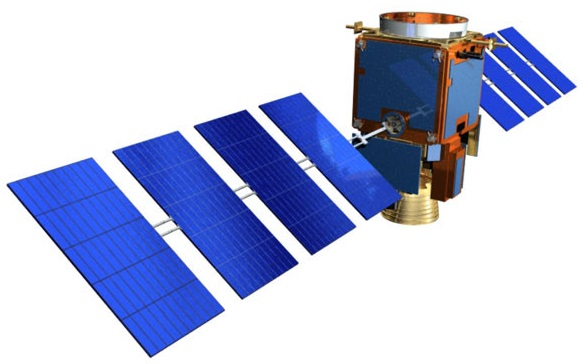
\includegraphics[width=\textwidth]{images/satellite.jpg}
\end{figure}
\column{0.5\textwidth}
\begin{figure}
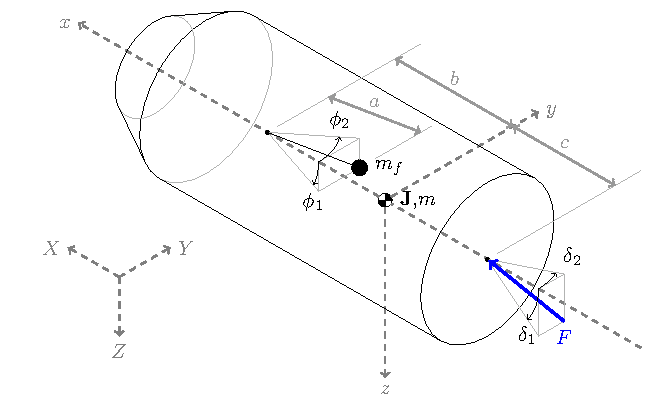
\includegraphics[width=\textwidth]{images/rocket3.pdf}
\end{figure}
\end{columns}
\end{frame}

%%%%%%%%%%%%%%%%%%%%%%%%%%%%%%%%%%%%%%%%%%%%%%%%%%%%%%%%%%%%%%%%%%%%%%%%%%%%
%%%%%%%%%%%%%%%%%%%%%%%%%-------PROBLEM STATEMENT--------%%%%%%%%%%%%%%%%%%%
%%%%%%%%%%%%%%%%%%%%%%%%%%%%%%%%%%%%%%%%%%%%%%%%%%%%%%%%%%%%%%%%%%%%%%%%%%%%
\section{Problem Statement}
\begin{frame}{Problem Statement}
Given a SISO (single-input single-output) undamped system described by:
\begin{equation}
\ddot{\mathbf{q}}(t) + \Lambda\mathbf{q}(t) = \mathbf{b}u(t)
\label{eq:modal1}
\end{equation}
\begin{equation}
y(t) = \mathbf{c}^T \mathbf{q}(t)
\label{eq:modal2}
\end{equation}
$$
\Lambda = \begin{bmatrix}
\lambda_1  &  0 & \cdots & 0 \\
0 & \lambda_2  & \ddots & 0 \\
\vdots & \ddots & \ddots & \vdots \\
0 & 0 & \cdots & \lambda_n \end{bmatrix}
,\quad \mathbf{b} = \begin{bmatrix} b_1 \\ b_2 \\ \vdots \\ b_n \end{bmatrix}
,\quad \mathbf{c} = \begin{bmatrix} c_1 \\ c_2 \\ \vdots \\ c_n \end{bmatrix}
\label{eq:modal3}
$$
where $u(t)$ is the input and $y(t)$ is the output,
\begin{enumerate}
\item Under what conditions can this system be transformed into a mass-spring string where the input is a force on first mass and output is the position of the first mass.
\item If so, how can the equivalent system (mass and stiffness values) be calculated?
\end{enumerate}
\end{frame}

\begin{frame}{Problem Statement}
In other words: Can we find a coordinate transformation $\mathbf{x} = P \mathbf{q}$, from $\mathbf{q}$ to a new coordinate system $\mathbf{x}$
such that:
\begin{equation}
M\ddot{\mathbf{x}}(t) + K\mathbf{x}(t) = \mathbf{\hat{b}}u(t)
\label{eq:ms1}
\end{equation}
\begin{equation}
y(t) = \mathbf{\hat{c}}^T \mathbf{x}(t)
\label{eq:ms2}
\end{equation}
\footnotesize{
$$
M = \begin{bmatrix}
m_1  &  0 & \cdots & 0 \\
0 & m_2  & \ddots & 0 \\
\vdots & \ddots & \ddots & \vdots \\
0 & 0 & \cdots & m_n \end{bmatrix}
, \quad
K = \begin{bmatrix}
k_0+k_1  &  -k_1  & \cdots & 0 \\
-k_1 & k_1+k_2   & \ddots & 0 \\
\vdots & \ddots & \ddots & -k_{n-1} \\
0 & 0  & -k_{n-1} &  k_{n-1} + k_n \end{bmatrix}
$$
$$
\mathbf{\hat{b}} = \begin{bmatrix} 1 & 0 & \cdots & 0 \end{bmatrix}^T
,\quad \mathbf{\hat{c}} = \begin{bmatrix} 1 & 0 & \cdots & 0 \end{bmatrix}^T
\label{eq:ms3}
$$
}
\end{frame}
%%%%% image of mass spring required form

%%%%%%%%%%%%%%%%%%%%%%%%%%%%%%%%%%%%%%%%%%%%%%%%%%%%%%%%%%%%%%%%%%%%%%%%%
%%%%%%%%%%%%%%%%%%%%%%%%%-------METHODS--------%%%%%%%%%%%%%%%%%%%%%%%%%%
%%%%%%%%%%%%%%%%%%%%%%%%%%%%%%%%%%%%%%%%%%%%%%%%%%%%%%%%%%%%%%%%%%%%%%%%%
\section{Methods}
\subsection{Inverse Eigenvalue Problem for Jacobi Matrices}
\begin{frame}
First consider the transformation $\mathbf{v} = A \mathbf{q}$
$$A = \begin{bmatrix}
a_1  &  0 & \cdots & 0 \\
0 & a_2  & \ddots & 0 \\
\vdots & \ddots & \ddots & \vdots \\
0 & 0 & \cdots & a_n \end{bmatrix}$$
Scales the $\mathbf{b}$ and $\mathbf{c}$ vectors without affecting $\Lambda$
\begin{equation}
\ddot{\mathbf{v}}(t) +  \Lambda \mathbf{v}(t) =  A^{-1} \mathbf{b}u(t) =  \begin{bmatrix} b_1/a_1 \\ b_2/a_2 \\ \vdots \\ b_n/a_n  \end{bmatrix} u(t)
\label{eq:scaled1}
\end{equation}
\begin{equation}
y(t) = \mathbf{c}^T  A \mathbf{v}(t) = \begin{bmatrix} a_1 c_1 & a_2 c_2 & \cdots & a_n c_n \end{bmatrix} \mathbf{v}(t)
\label{eq:scaled2}
\end{equation}
\end{frame}

\subsection{Mass Spring Reconstruction}
\begin{frame}
The final step is to reconstruct the mass and stiffness matrices $M$ and $K$.
It can be shown that $J =  M^{-\frac{1}{2}} K M^{-\frac{1}{2}}$ and the transformation $\mathbf{x} = M^{\frac{1}{2}} \mathbf{z}$ where $M$ has the form given in Eq. \ref{eq:ms3} leads to the final system:
\begin{equation}
M \ddot{\mathbf{x}}(t) + K \mathbf{x}(t) = M^{\frac{1}{2}} U A^{-1} \mathbf{b} u(t)
\label{eq:fin1}
\end{equation}
\begin{equation}
y(t) = \mathbf{c}^T  A U^T M^{\frac{1}{2}}\mathbf{x}(t)
\label{eq:fin2}
\end{equation}

The matrix $M$ is calculated as follows: We can write $K = M^{\frac{1}{2}} J M^{\frac{1}{2}}$ where $K$ and $M$ are mass and stiffness matrices of Eq. \ref{eq:ms3} which we want to calculate.
We will only consider here the case where $k_0 = k_n = 0$ and where $K$ (and $J$) are singular, corresponding to a free-free mass-spring system.
In this case one eigenvalue of the system $\lambda_1 = 0$.
The example we show later in the paper is indeed such a system.
The rows of $K$ must sum to zero. This can be written as
\begin{equation}
K \begin{bmatrix} 1 & 1 & \cdots & 1 \end{bmatrix}^T =  M^{\frac{1}{2}} J M^{\frac{1}{2}} \begin{bmatrix} 1 & 1 & \cdots & 1 \end{bmatrix}^T = \mathbf{0}
\end{equation} 
which may be rewritten as
\begin{equation}
J \begin{bmatrix} \sqrt{m_1} & \sqrt{m_2} & \cdots & \sqrt{m_n} \end{bmatrix}^T = \mathbf{0}
\end{equation}
Once a value is chosen for $m_1$ this equation may be solved row by row to calculate each $m_i$.
The values of the $k_i$ easily follow.
The correct choice for $m_1$ is shown in Eq. \ref{eq:bcxm} below.
\end{frame}


\subsection{Necessary and Sufficient Conditions for Transformation}
\begin{frame}
By comparing this system to that of Eqs. \ref{eq:ms1}-\ref{eq:ms3} we get the following equation for $\mathbf{b}$ and $\mathbf{c}$.
\begin{equation}
M^{\frac{1}{2}} U A^{-1} \mathbf{b} = M^{\frac{1}{2}} U A \mathbf{c} = \begin{bmatrix} 1 &  0 & \cdots & 0 \end{bmatrix}^T
\label{eq:bhat}
\end{equation}
which can be simplified to
\begin{equation}
A^{-1} \mathbf{b} = A \mathbf{c} = \frac{1}{m_1} U^T \begin{bmatrix} 1 &  0 & \cdots & 0 \end{bmatrix}^T
\label{eq:bc1}
\end{equation}
and then
\begin{equation}
A^{-1} \mathbf{b} = A \mathbf{c} = \frac{1}{m_1} \mathbf{x}_1
\label{eq:bc2}
\end{equation}
This can be solved to give
\begin{equation}
a_i = \sqrt{\frac{b_i}{c_i}} ,\quad m_1 = \sqrt{\frac{1}{\sum b_i c_i}} ,\quad x_{i1} = \sqrt{\frac{b_i c_i}{\sum b_i c_i}}
\label{eq:bcxm}
\end{equation}
By combining the three steps the overall transformation can be written as
\begin{equation}
P =  M^{-\frac{1}{2}} U A^{-1}
\label{eq:p}
\end{equation}
Examining Eq. \ref{eq:bcxm} we find that a second necessary and sufficient condition for $P$ to exist is
\begin{equation}
\frac{b_i}{c_i} > 0 \quad \forall i
\label{eq:bc1}
\end{equation}
that is, the sign of each $b_i$ term is the same as the corresponding $c_i$ term. 
Also note however that if
\begin{equation}
\frac{b_i}{c_i} < 0 \quad \forall i
\label{eq:bc2}
\end{equation}
then we can write down a new system by changing the signs of both $u(t)$ and $\mathbf{b}$. We then have a new system identical to the old system but where the input is $-u(t)$ and Eq. \ref{eq:bc1} is satisfied.
This condition may be summarized as: the corresponding entries in the $\mathbf{b}$ and $\mathbf{c}$ vectors must either all have the same sign or all have opposite signs.
\end{frame}

%%%%%%%%%%%%%%%%%%%%%%%%%%%%%%%%%%%%%%%%%%%%%%%%%%%%%%%%%%%%%%%%%%%%%%%%%
%%%%%%%%%%%%%%%%%%%%%%%%%-------RESULTS--------%%%%%%%%%%%%%%%%%%%%%%%%%%
%%%%%%%%%%%%%%%%%%%%%%%%%%%%%%%%%%%%%%%%%%%%%%%%%%%%%%%%%%%%%%%%%%%%%%%%%
\section{Results}

\subsection{Segmented Rocket Model}

\begin{frame}{Segmented rocket model}
\begin{columns} %%% check alignment in beamer columns
\column{0.5\textwidth}
\centering
%Styles
\tikzstyle{cog} = [draw=black, inner sep=0, minimum size = 0.2cm, circle, node distance=2cm, path picture={ 
      \filldraw[] (path picture bounding box.west) -- (path picture bounding box.east)-- (path picture bounding box.north east) -- (path picture bounding box.north) -- (path picture bounding box.south) -- (path picture bounding box.south west) -- cycle;}]
\tikzstyle{force}=[>=latex,draw=blue,fill=blue]
\tikzstyle{axis} =[dashed,gray,font=\small]

\begin{tikzpicture}[scale=0.75]
\def\h{2cm}
\def\w{1.5cm}
\def\thet{50}
\def\phio{-15}
\def\phit{-10}
\def\del{10}

%   Newtonian Ref frame 
 	\draw[axis,->]  (0,0) -- (0,-\w)  node[right]{$Z$};
 	\draw[axis,->]  (0,0) --  (-\w,0) node[left]{$X$};
 	\draw[draw=gray,->,] (-\w/2,0) node[above left]{$\theta$} arc (180 : 90+\thet : \w/2);
	
	\begin{scope}[yshift=0,rotate=\thet]
 	\draw[axis,->]  (0,-0.75*\h) -- (0,\w)  node[above]{$x$};
 	\draw[axis,->]  (0,0) --  (-\w,0) node[left]{$z$};
	\draw[] (-\w/2,0) rectangle (\w/2,\h);
	\node[cog] at (0,\h/2) {};	
	\draw[axis,-]  (-\w/2,\h) -- (-\w,\h);
	\draw[draw=gray,->,] (-\w,\h) node[below]{$\phi_1$} arc (180:180+\phio:\w);
	\draw[force,->] (\w,\h)  node[right]{$f_1$}  -- (\w/2,\h);
	
	\begin{scope}[yshift=\h,rotate=\phio]

	\draw[] (-\w/2,0) rectangle (\w/2,\h);
	\node[cog] at (0,\h/2) {};
	\node[] at  (0,0.7*\h) {$I$, $m$};
	\draw[axis,-]  (-\w/2,\h) -- (-\w,\h);
	\draw[axis,-]  (-\w/2,0) -- (-\w,0);
	\draw[draw=gray,->,] (-\w,\h) node[below]{$\phi_2$} arc (180:180+\phit:\w);
	\draw[force,->] (\w,\h)  node[right]{$f_2$}  -- (\w/2,\h);
	\draw [domain=0:12.56,variable=\t,smooth,samples=75] plot ({\t r}: {0.020*\t});
	\draw[draw=gray,<->,] (-0.75*\w,0)  -- node[left]{$h$} (-0.75*\w,\h);
	
	\begin{scope}[yshift=\h, rotate=\phit]
	\draw[axis,-]  (-\w/2,0) -- (-\w,0);
	\draw[] (-\w/2,0) -- (-\w/2,3*\h/4) -- (-\w/4,\h) -- (\w/4,\h) -- (\w/2,3*\h/4) -- (\w/2,0) --  (-\w/2,0) ;
	\node[cog] at (0,\h/2) {};	
	\draw[force,->] (3*\w/4,\h)  node[right]{$f_3$}  -- (\w/4,\h);
	\draw [domain=0:12.56,variable=\t,smooth,samples=75] plot ({\t r}: {0.020*\t});
	
	\end{scope}
	\end{scope}
	
	\begin{scope}[rotate = \del]
	\draw[]  (0,0) -- (-0.2*\w,-0.4*\h) -- (0.2*\w,-0.4*\h) -- cycle;
	\draw[force,->] (0,-\h)  node[right]{$T$}  -- (0,-0.4*\h);
	\filldraw (0,0) circle (1pt);
	\end{scope}
	\draw[draw=gray,->,] (0,-0.75*\h) node[below]{$\delta$} arc (-90:-90+\del:0.75*\h);

	\end{scope}


\end{tikzpicture} \\
Segmented rocket model
\column{0.5\textwidth}
\begin{itemize}
\item 3 rigid bodies, 2 torsional springs
\item 4 actuators - three lateral thruster forces $f_i$
\item gimballed engine thrust - $\delta$
\item Three outputs - attitude sensors on each segment - $\alpha_1$, $\alpha_2$ and $\alpha_3$
\end{itemize}
\end{columns}
\end{frame}

\begin{frame}{Segmented rocket model}
\begin{itemize}
\item Equations of motion:
\begin{multline}
\left[\begin{matrix}3 I + 2 h^{2} m & 2 I + \frac{3 m}{2} h^{2} & I + \frac{h^{2} m}{2}\\2 I + \frac{3 m}{2} h^{2} & 2 I + \frac{7 m}{6} h^{2} & I + \frac{5 m}{12} h^{2}\\I + \frac{h^{2} m}{2} & I + \frac{5 m}{12} h^{2} & I + \frac{h^{2} m}{6}\end{matrix}\right]\left[\begin{matrix}\ddot{\theta}\\\ddot{\phi}_{1}\\\ddot{\phi}_{2}\end{matrix}\right]\\ + \left[\begin{matrix}0 & - \frac{2 T}{3} h & - \frac{T h}{6}\\0 & - \frac{2 T}{3} h + k & - \frac{T h}{6}\\0 & - \frac{T h}{6} & - \frac{T h}{6} + k\end{matrix}\right]\left[\begin{matrix}\theta\\\phi_{1}\\\phi_{2}\end{matrix}\right] = \left[\begin{matrix}\frac{3 T}{2} h & \frac{h}{2} & - \frac{h}{2} & - \frac{3 h}{2}\\\frac{2 T}{3} h & \frac{2 h}{3} & - \frac{h}{3} & - \frac{4 h}{3}\\\frac{T h}{6} & \frac{h}{6} & \frac{h}{6} & - \frac{5 h}{6}\end{matrix}\right]\left[\begin{matrix}\delta\\f_{1}\\f_{2}\\f_{3}\end{matrix}\right]
\end{multline}
\item Output equation:
\begin{equation}
\left[\begin{matrix}\alpha_{1}\\\alpha_{2}\\\alpha_{3}\end{matrix}\right] = \left[\begin{matrix}1 & 0 & 0\\1 & 1 & 0\\1 & 1 & 1\end{matrix}\right]\left[\begin{matrix}\theta\\\phi_{1}\\\phi_{2}\end{matrix}\right]
\end{equation}
\item Choice of 4 actuators and 3 attitude sensors
\end{itemize}
\end{frame}

\begin{frame}{Model Parameters}
\begin{columns}
\column{0.3\textwidth}
\centering
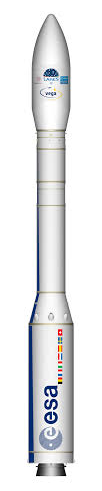
\includegraphics[height=0.75\textheight]{images/Vega.png} \\
Vega Rocket
\column{0.7\textwidth}
\begin{itemize}
\item Numerical values for model parameters representative of European \emph{Vega} rocket \footcite{Perez2006}
\item Chosen to match MOI, mass and first two vibration frequencies
\end{itemize}
\begin{table}
  \begin{center}
    \begin{tabular}{ ccc }
	\hline
           Parameter & Value & Unit \\
	\hline
      	$m$ & $5 \cdot 10^4$ & $kg$\\
      	$k$ & $6 \cdot 10^7$ & $Nm$\\
      	$I$ & $5 \cdot 10^5$ & $kg~m^2$\\
      	$h$ & $10$ & $m$\\
      	$T$ & $2.3 \cdot 10^6$ & $N$\\
    \end{tabular}
  \end{center}
\end{table}
\end{columns}

\end{frame}

\begin{frame}
Tab. \ref{tab:modelparam} presents numerical parameters for the model presented in Section \ref{sec:math-model} which are representative of the European launcher \emph{Vega} \cite{Perez2006}.
These values were substituted into the rocket equations of motion and then the system was diagonalised to have the same structure as Eqs. \ref{eq:modal1} to \ref{eq:modal3}.
\begin{multline}
\left[\begin{matrix}\ddot{q}_{1}\\\ddot{q}_{2}\\\ddot{q}_{3}\end{matrix}\right] + \left[\begin{matrix}0 & 0 & 0\\0 & 61.3 & 0\\0 & 0 & 309.0\end{matrix}\right]\left[\begin{matrix}q_{1}\\q_{2}\\q_{3}\end{matrix}\right] = \left[\begin{matrix}2.73 & 5.08 \cdot 10^{-7} & -4.08 \cdot 10^{-7} & -1.39 \cdot 10^{-6}\\-14.7 & 3.19 \cdot 10^{-6} & 3.19 \cdot 10^{-6} & -6.38 \cdot 10^{-6}\\19.9 & -1.05 \cdot 10^{-5} & 1.06 \cdot 10^{-5} & -8.93 \cdot 10^{-6}\end{matrix}\right]\left[\begin{matrix}\delta\\f_{1}\\f_{2}\\f_{3}\end{matrix}\right]
\label{eq:num_rock1}
\end{multline}
\begin{equation}
\left[\begin{matrix}\alpha_{1}\\\alpha_{2}\\\alpha_{3}\end{matrix}\right] = \left[\begin{matrix}1.0 & -0.592 & 0.322\\1.0 & -0.00814 & -0.347\\1.0 & 0.547 & 0.322\end{matrix}\right]\left[\begin{matrix}q_{1}\\q_{2}\\q_{3}\end{matrix}\right]
\label{eq:num_rock2}
\end{equation}
\end{frame}

\subsection{Test Cases for different sensor-actuator combinations}

\begin{frame}{Example Step Response}{Test Case 1}
\begin{columns}
\column{0.25\textwidth}
text
\column{0.75\textwidth}
    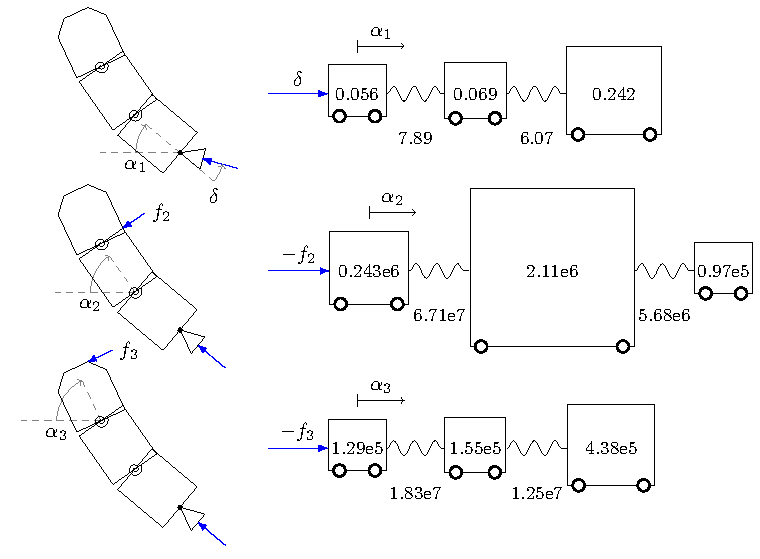
\includegraphics[width=\textwidth]{graphics/rocket-trans-pres.pdf}
\end{columns}
\end{frame}

\begin{frame}{Example Step Response}{Test Case 1}
\begin{center}
    %Styles
\tikzstyle{cog} = [draw=black, inner sep=0, minimum size = 0.2cm, circle, node distance=2cm, path picture={ 
      \filldraw[] (path picture bounding box.west) -- (path picture bounding box.east)-- (path picture bounding box.north east) -- (path picture bounding box.north) -- (path picture bounding box.south) -- (path picture bounding box.south west) -- cycle;}]
\tikzstyle{force}=[>=latex,draw=blue,fill=blue]
\tikzstyle{axis} =[dashed,gray,font=\small]
\tikzstyle{spring} = [black,decorate,decoration={snake,amplitude=3.5,segment length=10}]
\tikzstyle{cart} = [rectangle, inner sep=0,minimum height=0.8cm, minimum width=1cm, node distance=1.8cm, path picture={ 
      \draw[] ([yshift=0.12cm, xshift=0.3pt] path picture bounding box.south west) rectangle ([xshift=-0.3pt,yshift=-0.3pt] path picture bounding box.north east); 
      \draw[thick, fill=white] ([yshift=0.12cm, xshift=-0.2cm] path picture bounding box.south east) circle (0.1cm);
      \draw[thick,fill=white] ([yshift=0.12cm, xshift=0.2cm] path picture bounding box.south west) circle (0.1cm);
      }]

\begin{tikzpicture}[scale=1]

\def\h{1cm}
\def\w{0.9cm}
\def\thet{50}
\def\phio{-15}
\def\phit{-10}
\def\del{25}
\def\mw1{1cm}
\def\mh1{1cm}

	\begin{scope}[xshift=-2.7cm, yshift=1cm]
 	\draw[axis]  (0,0) --  (-1.5*\w,0) node[left]{};
	\draw[draw=gray,->,] (-0.75*\h,0) node[below]{$\alpha_1$} arc (180:90+\thet:0.75*\h);
	
	\begin{scope}[rotate=\thet]

 	\draw[axis]  (0,-0.75*\h) -- (0,0)  node[above]{};
 	\draw[axis]  (0,0) -- (0,0.75*\h)  node[above]{};
	\draw[] (-\w/2,0) rectangle (\w/2,\h);
	
	\begin{scope}[yshift=\h,rotate=\phio]
	\draw[] (-\w/2,0) rectangle (\w/2,\h);
	\draw [domain=0:12.56,variable=\t,smooth,samples=75] plot ({\t r}: {0.010*\t});
	
	\begin{scope}[yshift=\h, rotate=\phit]
	\draw[] (-\w/2,0) -- (-\w/2,3*\h/4) -- (-\w/4,\h) -- (\w/4,\h) -- (\w/2,3*\h/4) -- (\w/2,0) --  (-\w/2,0) ;
	\draw [domain=0:12.56,variable=\t,smooth,samples=75] plot ({\t r}: {0.010*\t});
	
	\end{scope}
	\end{scope}
	
	\begin{scope}[rotate = \del]
	\draw[]  (0,0) -- (-0.2*\w,-0.4*\h) -- (0.2*\w,-0.4*\h) -- cycle;
	\draw[force,->] (0,-\h)  node[right]{}  -- (0,-0.4*\h);
	\filldraw (0,0) circle (1pt);
	\end{scope}
	\draw[draw=gray,->,] (0,-0.75*\h) node[below]{$\delta$} arc (-90:-90+\del:0.75*\h);
	\end{scope}
	\end{scope}

\begin{axis}[%
width=5.5cm,
height=4cm,
at={(0cm,0cm)},
scale only axis,
separate axis lines,
every outer x axis line/.append style={black},
every x tick label/.append style={font=\color{black}},
xmin=0,
xmax=5,
xlabel={t},
every outer y axis line/.append style={black},
every y tick label/.append style={font=\color{black}},
ymin=-0.3,
ymax=1.1,
ylabel={Segment Attitude Angles},
title={$\text{Input }\delta\text{, output }\alpha{}_\text{1}$},
legend style={legend cell align=left,align=left,draw=black,anchor=south east,at={(0.98,0.02)}}
]
\addplot [color=blue,solid]
  table[row sep=crcr]{%
0	0\\
0.0166666666666667	0.00971264942401434\\
0.0333333333333333	0.0380944783195947\\
0.05	0.0829337654986286\\
0.0666666666666667	0.14074529763993\\
0.0833333333333333	0.207083349118696\\
0.1	0.276961979377579\\
0.116666666666667	0.345336928016792\\
0.133333333333333	0.407591964032794\\
0.15	0.459971402476971\\
0.166666666666667	0.49990819917396\\
0.183333333333333	0.52621141780686\\
0.2	0.539095343193615\\
0.216666666666667	0.540052358487463\\
0.233333333333333	0.531590325082866\\
0.25	0.516870408568779\\
0.266666666666667	0.49929147416408\\
0.283333333333333	0.482071427765081\\
0.3	0.467874045480766\\
0.316666666666667	0.458522461275793\\
0.333333333333333	0.454828709228656\\
0.35	0.456554113051831\\
0.366666666666667	0.462499679144376\\
0.383333333333333	0.470710796286143\\
0.4	0.478768107805349\\
0.416666666666667	0.484127681253419\\
0.433333333333333	0.484469363461597\\
0.45	0.478012745577922\\
0.466666666666667	0.463765204625051\\
0.483333333333333	0.441675284088764\\
0.5	0.412676097970702\\
0.516666666666667	0.378616126670382\\
0.533333333333333	0.342087278617189\\
0.55	0.306171061756416\\
0.566666666666667	0.274132013235891\\
0.583333333333333	0.249092381542273\\
0.6	0.233723058662153\\
0.616666666666667	0.229982967291026\\
0.633333333333333	0.238932972713489\\
0.65	0.26064170303153\\
0.666666666666667	0.294190456189415\\
0.683333333333333	0.337773796733497\\
0.7	0.388882637997269\\
0.716666666666667	0.444548573385764\\
0.733333333333333	0.501622737601588\\
0.75	0.557060014078096\\
0.766666666666667	0.60818008673587\\
0.783333333333333	0.652880451710784\\
0.8	0.689782546221229\\
0.816666666666667	0.71829987282051\\
0.833333333333333	0.738625510518452\\
0.85	0.751644780018929\\
0.866666666666667	0.758786197206656\\
0.883333333333333	0.761829483390697\\
0.9	0.762692796392193\\
0.916666666666667	0.763222257628672\\
0.933333333333333	0.765005305225819\\
0.95	0.769225688022898\\
0.966666666666667	0.776572531280089\\
0.983333333333333	0.787209504548132\\
1	0.800803433035469\\
1.01666666666667	0.816605437550496\\
1.03333333333333	0.833572504264998\\
1.05	0.850513767826421\\
1.06666666666667	0.866244042383288\\
1.08333333333333	0.879727343809487\\
1.1	0.890195189191153\\
1.11666666666667	0.897228023980727\\
1.13333333333333	0.900792754378997\\
1.15	0.901234503551958\\
1.16666666666667	0.899225789038582\\
1.18333333333333	0.895680794439027\\
1.2	0.891645831812885\\
1.21666666666667	0.888179147532756\\
1.23333333333333	0.886233760668548\\
1.25	0.886556056409332\\
1.26666666666667	0.889610564541893\\
1.28333333333333	0.895538044765481\\
1.3	0.904150080382374\\
1.31666666666667	0.914959299343933\\
1.33333333333333	0.927240542123251\\
1.35	0.940115173148797\\
1.36666666666667	0.952648589098615\\
1.38333333333333	0.963949996658112\\
1.4	0.973263764874536\\
1.41666666666667	0.980043021528409\\
1.43333333333333	0.983998460571853\\
1.45	0.985118270054513\\
1.46666666666667	0.983658333366734\\
1.48333333333333	0.980105041545\\
1.5	0.975115844519335\\
1.51666666666667	0.969444786214851\\
1.53333333333333	0.963861518873982\\
1.55	0.959072583763111\\
1.56666666666667	0.955653092845162\\
1.58333333333333	0.953995463067735\\
1.6	0.954279738508689\\
1.61666666666667	0.956467540541177\\
1.63333333333333	0.960319095277505\\
1.65	0.965430380289191\\
1.66666666666667	0.971285455497469\\
1.68333333333333	0.977317685126585\\
1.7	0.982972932760373\\
1.71666666666667	0.987767950481802\\
1.73333333333333	0.991338033809053\\
1.75	0.993469451561625\\
1.76666666666667	0.99411400251848\\
1.78333333333333	0.993385083136241\\
1.8	0.991536647388941\\
1.81666666666667	0.988928190454106\\
1.83333333333333	0.985980218434214\\
1.85	0.983125455694795\\
1.86666666666667	0.980761232318321\\
1.88333333333333	0.97920809570633\\
1.9	0.978678773891306\\
1.91666666666667	0.979260306687795\\
1.93333333333333	0.980910613513447\\
1.95	0.983469159999409\\
1.96666666666667	0.986679893566994\\
1.98333333333333	0.990223394443847\\
2	0.993754350548634\\
2.01666666666667	0.99694008290378\\
2.03333333333333	0.999495941301023\\
2.05	1.00121392489764\\
2.06666666666667	1.00198178081514\\
2.08333333333333	1.00179098226252\\
2.1	1.0007332516615\\
2.11666666666667	0.998986533354432\\
2.13333333333333	0.996792403795432\\
2.15	0.994427726653773\\
2.16666666666667	0.992173841305231\\
2.18333333333333	0.990286680731678\\
2.2	0.988970955353516\\
2.21666666666667	0.988360958039417\\
2.23333333333333	0.988509719829854\\
2.25	0.989387275445313\\
2.26666666666667	0.990887792718687\\
2.28333333333333	0.992844389349734\\
2.3	0.995049699354467\\
2.31666666666667	0.997279733132675\\
2.33333333333333	0.999318342728133\\
2.35	1.00097966858068\\
2.36666666666667	1.00212628468815\\
2.38333333333333	1.00268132608384\\
2.4	1.00263360466037\\
2.41666666666667	1.0020355123262\\
2.43333333333333	1.00099428648917\\
2.45	0.999657890185268\\
2.46666666666667	0.998197270524515\\
2.48333333333333	0.996787058135155\\
2.5	0.995586835420082\\
2.51666666666667	0.994724937092042\\
2.53333333333333	0.994286381233969\\
2.55	0.994306011637632\\
2.56666666666667	0.99476732486129\\
2.58333333333333	0.995606827303897\\
2.6	0.99672318648374\\
2.61666666666667	0.997989966202897\\
2.63333333333333	0.999270412711324\\
2.65	1.00043261532011\\
2.66666666666667	1.00136340676443\\
2.68333333333333	1.00197958252419\\
2.7	1.00223537314879\\
2.71666666666667	1.00212555478029\\
2.73333333333333	1.00168407781048\\
2.75	1.00097857714008\\
2.76666666666667	1.00010154887653\\
2.78333333333333	0.999159295643784\\
2.8	0.998259927220595\\
2.81666666666667	0.997501741745791\\
2.83333333333333	0.996963208192193\\
2.85	0.996695541270677\\
2.86666666666667	0.996718535875947\\
2.88333333333333	0.997019948710648\\
2.9	0.997558322921378\\
2.91666666666667	0.998268789775696\\
2.93333333333333	0.9990710866892\\
2.95	0.99987883142576\\
2.96666666666667	1.0006090046896\\
2.98333333333333	1.00119062153387\\
3	1.00157170743325\\
3.01666666666667	1.00172391791197\\
3.03333333333333	1.00164442330447\\
3.05	1.00135498957445\\
3.06666666666667	1.00089848790414\\
3.08333333333333	1.00033332822315\\
3.1	0.999726508929139\\
3.11666666666667	0.999146088935242\\
3.13333333333333	0.998653910754537\\
3.15	0.99829933660573\\
3.16666666666667	0.998114614913536\\
3.18333333333333	0.998112291239262\\
3.2	0.99828484009534\\
3.21666666666667	0.99860644921857\\
3.23333333333333	0.999036662121278\\
3.25	0.999525401215335\\
3.26666666666667	1.00001877000582\\
3.28333333333333	1.00046497906943\\
3.3	1.0008197591065\\
3.31666666666667	1.0010507098073\\
3.33333333333333	1.00114017327074\\
3.35	1.00108639771399\\
3.36666666666667	1.00090295058033\\
3.38333333333333	1.00061652851189\\
3.4	1.00026347519201\\
3.41666666666667	0.999885440569668\\
3.43333333333333	0.999524685396878\\
3.45	0.999219548364022\\
3.46666666666667	0.999000550746149\\
3.48333333333333	0.998887522584226\\
3.5	0.998888007043996\\
3.51666666666667	0.998997051050422\\
3.53333333333333	0.999198337428439\\
3.55	0.999466473077159\\
3.56666666666667	0.999770133558587\\
3.58333333333333	1.00007568776316\\
3.6	1.00035089338182\\
3.61666666666667	1.00056826615704\\
3.63333333333333	1.00070777981515\\
3.65	1.00075864144071\\
3.66666666666667	1.00071999784518\\
3.68333333333333	1.0006005493003\\
3.7	1.00041716450206\\
3.71666666666667	1.00019269245294\\
3.73333333333333	0.99995324301506\\
3.75	0.999725251338672\\
3.76666666666667	0.999532649160903\\
3.78333333333333	0.999394438991003\\
3.8	0.999322910004987\\
3.81666666666667	0.999322654613726\\
3.83333333333333	0.999390451743067\\
3.85	0.999515987397967\\
3.86666666666667	0.999683295362471\\
3.88333333333333	0.999872729878918\\
3.9	1.00006323460575\\
3.91666666666667	1.00023465200162\\
3.93333333333333	1.0003698253454\\
3.95	1.0004562796557\\
3.96666666666667	1.00048732293616\\
3.98333333333333	1.00046247855225\\
4	1.00038723506577\\
4.01666666666667	1.0002721731787\\
4.03333333333333	1.00013159286685\\
4.05	0.999981811041457\\
4.06666666666667	0.999839326914706\\
4.08333333333333	0.999719056791326\\
4.1	0.999632822859126\\
4.11666666666667	0.999588244579522\\
4.13333333333333	0.999588131226205\\
4.15	0.999630415995626\\
4.16666666666667	0.999708612495916\\
4.18333333333333	0.999812719730874\\
4.2	0.999930457517389\\
4.21666666666667	1.00004868480344\\
4.23333333333333	1.00015484101627\\
4.25	1.00023825585158\\
4.26666666666667	1.00029119439993\\
4.28333333333333	1.00030953912522\\
4.3	1.0002930536406\\
4.31666666666667	1.00024522041928\\
4.33333333333333	1.00017269032492\\
4.35	1.00008442134723\\
4.36666666666667	0.999990613279588\\
4.38333333333333	0.999901561642489\\
4.4	0.999826556793444\\
4.41666666666667	0.99977294326357\\
4.43333333333333	0.999745431738797\\
4.45	0.999745724734616\\
4.46666666666667	0.999772480660747\\
4.48333333333333	0.999821603747471\\
4.5	0.99988681321442\\
4.51666666666667	0.999960417583552\\
4.53333333333333	1.00003420177707\\
4.55	1.00010032709685\\
4.56666666666667	1.00015214763954\\
4.58333333333333	1.00018486026099\\
4.6	1.00019592693284\\
4.61666666666667	1.00018523552432\\
4.63333333333333	1.00015499453467\\
4.65	1.00010938584466\\
4.66666666666667	1.00005402415607\\
4.68333333333333	0.999995290017011\\
4.7	0.99993961355663\\
4.71666666666667	0.99989278757155\\
4.73333333333333	0.999859381679477\\
4.75	0.999842315027262\\
4.76666666666667	0.999842625379895\\
4.78333333333333	0.999859449679251\\
4.8	0.99989020791661\\
4.81666666666667	0.999930960910455\\
4.83333333333333	0.999976895487313\\
4.85	1.00002287924737\\
4.86666666666667	1.00006402248364\\
4.88333333333333	1.00009618708088\\
4.9	1.00011639077533\\
4.91666666666667	1.00012306879354\\
4.93333333333333	1.00011617191069\\
4.95	1.00009709839873\\
4.96666666666667	1.00006847514344\\
4.98333333333333	1.00003381852997\\
5	0.999997117018205\\
};
\addlegendentry{$\alpha{}_\text{1}$};

\addplot [color=red,dash pattern=on 1pt off 3pt on 3pt off 3pt]
  table[row sep=crcr]{%
0	0\\
0.0166666666666667	-0.00219086923091205\\
0.0333333333333333	-0.00836031954374985\\
0.05	-0.0173418492280184\\
0.0666666666666667	-0.027334259261131\\
0.0833333333333333	-0.0361080371079925\\
0.1	-0.0412692467203483\\
0.116666666666667	-0.0405513238478329\\
0.133333333333333	-0.0321003929569906\\
0.15	-0.0147198157543556\\
0.166666666666667	0.0119556677266637\\
0.183333333333333	0.0473774700720048\\
0.2	0.0901027408906008\\
0.216666666666667	0.137914426425894\\
0.233333333333333	0.188028664757502\\
0.25	0.237366563714918\\
0.266666666666667	0.282860424991194\\
0.283333333333333	0.321761031776025\\
0.3	0.351912984079227\\
0.316666666666667	0.371969080783416\\
0.333333333333333	0.38152184490278\\
0.35	0.381139584208838\\
0.366666666666667	0.372304782155728\\
0.383333333333333	0.357262954801276\\
0.4	0.338799272171656\\
0.416666666666667	0.319967283313507\\
0.433333333333333	0.303798325957561\\
0.45	0.293021295394773\\
0.466666666666667	0.289820395493866\\
0.483333333333333	0.295653636356802\\
0.5	0.311147801485514\\
0.516666666666667	0.336077211910461\\
0.533333333333333	0.369424803161263\\
0.55	0.409515744495831\\
0.566666666666667	0.45420691305917\\
0.583333333333333	0.501110651254353\\
0.6	0.547828802217844\\
0.616666666666667	0.592173177349459\\
0.633333333333333	0.632351223421262\\
0.65	0.667100335147917\\
0.666666666666667	0.695760413730779\\
0.683333333333333	0.71828118710213\\
0.7	0.735167722236346\\
0.716666666666667	0.747373749964984\\
0.733333333333333	0.75615727614074\\
0.75	0.762916028839349\\
0.766666666666667	0.769021358136439\\
0.783333333333333	0.775668255099235\\
0.8	0.783756395728173\\
0.816666666666667	0.793812930549479\\
0.833333333333333	0.80596264943245\\
0.85	0.819945741721749\\
0.866666666666667	0.835178235534332\\
0.883333333333333	0.850845869519397\\
0.9	0.866019045185544\\
0.916666666666667	0.879774895953034\\
0.933333333333333	0.891312485569348\\
0.95	0.900048634370135\\
0.966666666666667	0.90568463086026\\
0.983333333333333	0.908237757845238\\
1	0.908035706888756\\
1.01666666666667	0.905676103519439\\
1.03333333333333	0.901957072394251\\
1.05	0.897787659799381\\
1.06666666666667	0.894088729743114\\
1.08333333333333	0.891695518570764\\
1.1	0.891272369133596\\
1.11666666666667	0.893248398750125\\
1.13333333333333	0.897780226999269\\
1.15	0.904744721893369\\
1.16666666666667	0.913761380649142\\
1.18333333333333	0.924240809952458\\
1.2	0.935453138413625\\
1.21666666666667	0.946608338002506\\
1.23333333333333	0.956939513808063\\
1.25	0.965780296890018\\
1.26666666666667	0.972628489255429\\
1.28333333333333	0.977189911566588\\
1.3	0.979398764819534\\
1.31666666666667	0.979413459928123\\
1.33333333333333	0.977589499985569\\
1.35	0.974433340206659\\
1.36666666666667	0.970542965552414\\
1.38333333333333	0.966542048157959\\
1.4	0.963014889890935\\
1.41666666666667	0.960448920487274\\
1.43333333333333	0.959190392177004\\
1.45	0.959417240728836\\
1.46666666666667	0.961131073741013\\
1.48333333333333	0.964168129217066\\
1.5	0.968227050867695\\
1.51666666666667	0.972909657042157\\
1.53333333333333	0.977769698847054\\
1.55	0.982364011289506\\
1.56666666666667	0.986300493026908\\
1.58333333333333	0.989277971448251\\
1.6	0.991114125295795\\
1.61666666666667	0.991759103889699\\
1.63333333333333	0.991294126895155\\
1.65	0.989915987668589\\
1.66666666666667	0.987909842342597\\
1.68333333333333	0.985613799443409\\
1.7	0.983379526388942\\
1.71666666666667	0.981533306115821\\
1.73333333333333	0.980341709992089\\
1.75	0.979985354276639\\
1.76666666666667	0.980543172335598\\
1.78333333333333	0.981988390429332\\
1.8	0.984196084089242\\
1.81666666666667	0.986960957985655\\
1.83333333333333	0.990022962699919\\
1.85	0.993097636887902\\
1.86666666666667	0.995907705581768\\
1.88333333333333	0.998212495271117\\
1.9	0.999832122070393\\
1.91666666666667	1.00066411091916\\
1.93333333333333	1.00069102184753\\
1.95	0.999978685588752\\
1.96666666666667	0.998665670641192\\
1.98333333333333	0.99694550888011\\
2	0.995043906053803\\
2.01666666666667	0.993193592323052\\
2.03333333333333	0.991609593685783\\
2.05	0.990467528802362\\
2.06666666666667	0.989887090642537\\
2.08333333333333	0.989922218777675\\
2.1	0.990558685609189\\
2.11666666666667	0.991718997824234\\
2.13333333333333	0.99327374226786\\
2.15	0.99505786296952\\
2.16666666666667	0.996889905373838\\
2.18333333333333	0.998592043612054\\
2.2	1.00000872922909\\
2.21666666666667	1.00102205103793\\
2.23333333333333	1.00156233794056\\
2.25	1.00161311337438\\
2.26666666666667	1.00121015364543\\
2.28333333333333	1.00043504110002\\
2.3	0.999404169159461\\
2.31666666666667	0.998254592997144\\
2.33333333333333	0.997128386877681\\
2.35	0.996157246695632\\
2.36666666666667	0.995448965007426\\
2.38333333333333	0.995077126849256\\
2.4	0.995074965717881\\
2.41666666666667	0.995433830096456\\
2.43333333333333	0.996106197777795\\
2.45	0.997012693774037\\
2.46666666666667	0.998052167528888\\
2.48333333333333	0.999113605114632\\
2.5	1.00008851609512\\
2.51666666666667	1.00088245026224\\
2.53333333333333	1.00142445750356\\
2.55	1.00167358088837\\
2.56666666666667	1.00162183342533\\
2.58333333333333	1.00129351041493\\
2.6	1.00074108713884\\
2.61666666666667	1.00003830359583\\
2.63333333333333	0.99927130883603\\
2.65	0.998528902233717\\
2.66666666666667	0.997892955347028\\
2.68333333333333	0.997430026632282\\
2.7	0.997185005500266\\
2.71666666666667	0.997177365785465\\
2.73333333333333	0.997400302851076\\
2.75	0.997822708233222\\
2.76666666666667	0.998393635749891\\
2.78333333333333	0.999048664329026\\
2.8	0.999717389451737\\
2.81666666666667	1.00033119188781\\
2.83333333333333	1.00083044383388\\
2.85	1.00117041286582\\
2.86666666666667	1.00132529831841\\
2.88333333333333	1.00129006069479\\
2.9	1.00107995592511\\
2.91666666666667	1.00072793477708\\
2.93333333333333	1.00028028714861\\
2.95	0.999791079388919\\
2.96666666666667	0.999316034734807\\
2.98333333333333	0.998906534772921\\
3	0.998604374166008\\
3.01666666666667	0.998437790125825\\
3.03333333333333	0.998419127213019\\
3.05	0.998544306547802\\
3.06666666666667	0.99879406828876\\
3.08333333333333	0.999136769017205\\
3.1	0.999532360751918\\
3.11666666666667	0.999937070641803\\
3.13333333333333	1.00030824911909\\
3.15	1.00060886217096\\
3.16666666666667	1.00081116670193\\
3.18333333333333	1.00089921728986\\
3.2	1.00086999411686\\
3.21666666666667	1.00073309886517\\
3.23333333333333	1.00050912043811\\
3.25	1.00022690908064\\
3.26666666666667	0.999920102165972\\
3.28333333333333	0.999623307984877\\
3.3	0.99936837062338\\
3.31666666666667	0.999181109898757\\
3.33333333333333	0.999078860663836\\
3.35	0.999069034963785\\
3.36666666666667	0.999148810782092\\
3.38333333333333	0.999305926109597\\
3.4	0.999520440377157\\
3.41666666666667	0.999767228933029\\
3.43333333333333	1.00001890949782\\
3.45	1.00024886806883\\
3.46666666666667	1.00043405721574\\
3.48333333333333	1.00055727974333\\
3.5	1.00060873936015\\
3.51666666666667	1.00058672859002\\
3.53333333333333	1.00049742229798\\
3.55	1.00035384196397\\
3.56666666666667	1.00017414098879\\
3.58333333333333	0.999979426352956\\
3.6	0.999791370916268\\
3.61666666666667	0.999629880655912\\
3.63333333333333	0.999511062526787\\
3.65	0.999445694754959\\
3.66666666666667	0.999438338135674\\
3.68333333333333	0.99948715197034\\
3.7	0.999584400186395\\
3.71666666666667	0.999717560406562\\
3.73333333333333	0.999870888761557\\
3.75	1.00002725183897\\
3.76666666666667	1.000170017841\\
3.78333333333333	1.00028480277441\\
3.8	1.00036089280303\\
3.81666666666667	1.00039220701948\\
3.83333333333333	1.00037772038533\\
3.85	1.00032132794245\\
3.86666666666667	1.00023119179559\\
3.88333333333333	1.000118665425\\
3.9	0.999996930312501\\
3.91666666666667	0.999879503962478\\
3.93333333333333	0.999778784394865\\
3.95	0.999704784316788\\
3.96666666666667	0.999664180571582\\
3.98333333333333	0.999659764818672\\
4	0.999690334518614\\
4.01666666666667	0.999751014525594\\
4.03333333333333	0.999833954209288\\
4.05	0.999929307706948\\
4.06666666666667	1.00002637922885\\
4.08333333333333	1.00011480347666\\
4.1	1.00018563378011\\
4.11666666666667	1.00023222654454\\
4.13333333333333	1.0002508376781\\
4.15	1.0002408814141\\
4.16666666666667	1.00020484028925\\
4.18333333333333	1.00014785272751\\
4.2	1.00007703772833\\
4.21666666666667	1.00000064127511\\
4.23333333333333	0.999927103971844\\
4.25	0.999864152993227\\
4.26666666666667	0.999818013861598\\
4.28333333333333	0.99979282018823\\
4.3	0.99979027466108\\
4.31666666666667	0.999809585233896\\
4.33333333333333	0.999847670011653\\
4.35	0.999899596032408\\
4.36666666666667	0.999959193923983\\
4.38333333333333	1.00001977449255\\
4.4	1.00007486602148\\
4.41666666666667	1.0001188927799\\
4.43333333333333	1.00014772534289\\
4.45	1.00015905032843\\
4.46666666666667	1.00015252891567\\
4.48333333333333	1.00012973747892\\
4.5	1.00009390719165\\
4.51666666666667	1.000049500044\\
4.53333333333333	1.00000167432367\\
4.55	0.999955701813795\\
4.56666666666667	0.999916401092409\\
4.58333333333333	0.999887646490157\\
4.6	0.999872001328133\\
4.61666666666667	0.999870508474335\\
4.63333333333333	0.999882652909952\\
4.65	0.999906491972285\\
4.66666666666667	0.999938931297994\\
4.68333333333333	0.999976110040221\\
4.7	1.00001384906014\\
4.71666666666667	1.00004811132746\\
4.73333333333333	1.00007542491941\\
4.75	1.00009322538912\\
4.76666666666667	1.00010008494986\\
4.78333333333333	1.00009580954653\\
4.8	1.00008139986818\\
4.81666666666667	1.00005888703235\\
4.83333333333333	1.00003106649758\\
4.85	1.00000116345727\\
4.86666666666667	0.999972468655641\\
4.88333333333333	0.999947984832739\\
4.9	0.999930120929648\\
4.91666666666667	0.999920464304297\\
4.93333333333333	0.999919651439483\\
4.95	0.999927346147421\\
4.96666666666667	0.999942322394144\\
4.98333333333333	0.999962637866792\\
5	0.999985875415984\\
};
\addlegendentry{$\alpha{}_\text{2}$};

\addplot [color=black,dashed]
  table[row sep=crcr]{%
0	0\\
0.0166666666666667	0.000586064016735837\\
0.0333333333333333	0.00209990833471416\\
0.05	0.00384198296796189\\
0.0666666666666667	0.00475557072197379\\
0.0833333333333333	0.0035801165990626\\
0.1	-0.000957021623641259\\
0.116666666666667	-0.00993299819225336\\
0.133333333333333	-0.0240315093795191\\
0.15	-0.0433794500001077\\
0.166666666666667	-0.0674396580205676\\
0.183333333333333	-0.0949749855824499\\
0.2	-0.124090848266523\\
0.216666666666667	-0.152354454286023\\
0.233333333333333	-0.17698017210515\\
0.25	-0.195062972064219\\
0.266666666666667	-0.203836416588818\\
0.283333333333333	-0.200928855462898\\
0.3	-0.184591572589463\\
0.316666666666667	-0.153875560586412\\
0.333333333333333	-0.108738988647303\\
0.35	-0.0500746377888442\\
0.366666666666667	0.0203452122973757\\
0.383333333333333	0.100000649809674\\
0.4	0.185819426698203\\
0.416666666666667	0.274416381355871\\
0.433333333333333	0.362353835753717\\
0.45	0.446398424823616\\
0.466666666666667	0.523750946185677\\
0.483333333333333	0.592229261555112\\
0.5	0.650389595868229\\
0.516666666666667	0.697578146965077\\
0.533333333333333	0.733912013162785\\
0.55	0.760195319658222\\
0.566666666666667	0.777782384424213\\
0.583333333333333	0.788404243057517\\
0.6	0.793977462606363\\
0.616666666666667	0.796414741583092\\
0.633333333333333	0.797455362582516\\
0.65	0.798530385998778\\
0.666666666666667	0.800672968316651\\
0.683333333333333	0.804478893347885\\
0.7	0.810116911425199\\
0.716666666666667	0.817383371737217\\
0.733333333333333	0.825791417752369\\
0.75	0.834682085172688\\
0.766666666666667	0.843343230326844\\
0.783333333333333	0.851122385976698\\
0.8	0.857521282529857\\
0.816666666666667	0.862262626986725\\
0.833333333333333	0.865323426128342\\
0.85	0.866933231720363\\
0.866666666666667	0.867539712470788\\
0.883333333333333	0.867747490149353\\
0.9	0.868238861282692\\
0.916666666666667	0.869686616352663\\
0.933333333333333	0.87266955071933\\
0.95	0.877600456601796\\
0.966666666666667	0.884674541076194\\
0.983333333333333	0.893843583378449\\
1	0.904818050281933\\
1.01666666666667	0.917096189318533\\
1.03333333333333	0.930016168308344\\
1.05	0.942824934597532\\
1.06666666666667	0.954755862505614\\
1.08333333333333	0.965106580588846\\
1.1	0.973308653011435\\
1.11666666666667	0.978981958579938\\
1.13333333333333	0.981968502043735\\
1.15	0.982342770486993\\
1.16666666666667	0.980398337000793\\
1.18333333333333	0.976612928327742\\
1.2	0.97159634787413\\
1.21666666666667	0.966027263807851\\
1.23333333333333	0.960585786534538\\
1.25	0.955888904986505\\
1.26666666666667	0.952435246049411\\
1.28333333333333	0.950564364116471\\
1.3	0.950434020942282\\
1.31666666666667	0.952016886775728\\
1.33333333333333	0.955116009550928\\
1.35	0.95939648221673\\
1.36666666666667	0.964429183338701\\
1.38333333333333	0.969741419620998\\
1.4	0.97486884682913\\
1.41666666666667	0.979403206559946\\
1.43333333333333	0.983031143387412\\
1.45	0.985560555429766\\
1.46666666666667	0.986932432880606\\
1.48333333333333	0.987217779170924\\
1.5	0.986600807694441\\
1.51666666666667	0.985350996273189\\
1.53333333333333	0.983787625026206\\
1.55	0.982241027753095\\
1.56666666666667	0.981014910319309\\
1.58333333333333	0.980353742991746\\
1.6	0.980418477783107\\
1.61666666666667	0.981272777719128\\
1.63333333333333	0.982880701433343\\
1.65	0.985115505220757\\
1.66666666666667	0.987778044261516\\
1.68333333333333	0.990622296178152\\
1.7	0.993384884811399\\
1.71666666666667	0.995815203576642\\
1.73333333333333	0.997702837728514\\
1.75	0.998899434083258\\
1.76666666666667	0.999332900146344\\
1.78333333333333	0.999012739921613\\
1.8	0.998026342686635\\
1.81666666666667	0.996527021770517\\
1.83333333333333	0.994715449358884\\
1.85	0.992816766130841\\
1.86666666666667	0.991056003802901\\
1.88333333333333	0.989634519057875\\
1.9	0.988709906621713\\
1.91666666666667	0.988381375853584\\
1.93333333333333	0.988681902679907\\
1.95	0.989577687707543\\
1.96666666666667	0.990974650278513\\
1.98333333333333	0.992730953381027\\
2	0.994673960835149\\
2.01666666666667	0.99661963250829\\
2.03333333333333	0.998392198202932\\
2.05	0.999842022904469\\
2.06666666666667	1.00085986632948\\
2.08333333333333	1.00138620690845\\
2.1	1.00141488635622\\
2.11666666666667	1.0009909678597\\
2.13333333333333	1.00020331852846\\
2.15	0.999172960415145\\
2.16666666666667	0.998038631461435\\
2.18333333333333	0.996941222574833\\
2.2	0.996008794127036\\
2.21666666666667	0.995343729644865\\
2.23333333333333	0.995013280663081\\
2.25	0.995044334605086\\
2.26666666666667	0.995422747775777\\
2.28333333333333	0.996097083457125\\
2.3	0.996986134680099\\
2.31666666666667	0.997989239439647\\
2.33333333333333	0.998998148148027\\
2.35	0.999909099322735\\
2.36666666666667	1.00063380388461\\
2.38333333333333	1.00110821904002\\
2.4	1.00129828366151\\
2.41666666666667	1.00120215199964\\
2.43333333333333	1.00084885898134\\
2.45	1.00029373451612\\
2.46666666666667	0.999611215809638\\
2.48333333333333	0.998885952904848\\
2.5	0.998203241446503\\
2.51666666666667	0.997639838424814\\
2.53333333333333	0.99725612475677\\
2.55	0.997090388312969\\
2.56666666666667	0.997155737433745\\
2.58333333333333	0.997439849739018\\
2.6	0.99790744866855\\
2.61666666666667	0.998505114328535\\
2.63333333333333	0.999167805052017\\
2.65	0.999826313446514\\
2.66666666666667	1.00041481812963\\
2.68333333333333	1.00087772217077\\
2.7	1.00117508383874\\
2.71666666666667	1.00128612831417\\
2.73333333333333	1.00121055776838\\
2.75	1.00096762507401\\
2.76666666666667	1.00059317608304\\
2.78333333333333	1.00013507175523\\
2.8	0.999647554079671\\
2.81666666666667	0.999185205034215\\
2.83333333333333	0.998797159935274\\
2.85	0.99852217768095\\
2.86666666666667	0.998385050266791\\
2.88333333333333	0.998394668295517\\
2.9	0.998543867836921\\
2.91666666666667	0.998810988528735\\
2.93333333333333	0.999162894243743\\
2.95	0.999559064169782\\
2.96666666666667	0.999956267331373\\
2.98333333333333	1.00031329516262\\
3	1.000595246082\\
3.01666666666667	1.00077692826763\\
3.03333333333333	1.0008450617369\\
3.05	1.00079910410241\\
3.06666666666667	1.00065067938476\\
3.08333333333333	1.00042173894425\\
3.1	1.000141712274\\
3.11666666666667	0.999844000395222\\
3.13333333333333	0.999562217431909\\
3.15	0.999326593034315\\
3.16666666666667	0.999160911130719\\
3.18333333333333	0.999080285120058\\
3.2	0.999089965948762\\
3.21666666666667	0.999185259953103\\
3.23333333333333	0.999352511394527\\
3.25	0.999570993372095\\
3.26666666666667	0.999815461590552\\
3.28333333333333	1.00005906672747\\
3.3	1.00027629765817\\
3.31666666666667	1.00044564035794\\
3.33333333333333	1.00055168282527\\
3.35	1.00058646841546\\
3.36666666666667	1.00054998958459\\
3.38333333333333	1.00044981082761\\
3.4	1.00029990289721\\
3.41666666666667	1.00011885044345\\
3.43333333333333	0.999927654133608\\
3.45	0.999747380843786\\
3.46666666666667	0.999596919468657\\
3.48333333333333	0.99949107623346\\
3.5	0.999439195965945\\
3.51666666666667	0.999444430794078\\
3.53333333333333	0.999503702946423\\
3.55	0.999608332183115\\
3.56666666666667	0.999745229049975\\
3.58333333333333	0.999898499679879\\
3.6	1.0000512715002\\
3.61666666666667	1.00018753489187\\
3.63333333333333	1.00029380404314\\
3.65	1.00036042898881\\
3.66666666666667	1.00038243607056\\
3.68333333333333	1.00035983018135\\
3.7	1.00029735266551\\
3.71666666666667	1.00020374698251\\
3.73333333333333	1.00009063411664\\
3.75	0.999971136320462\\
3.76666666666667	0.999858407863026\\
3.78333333333333	0.999764233673471\\
3.8	0.9996978417558\\
3.81666666666667	0.999665045432171\\
3.83333333333333	0.99966779074119\\
3.85	0.999704137538273\\
3.86666666666667	0.999768655290186\\
3.88333333333333	0.999853171325772\\
3.9	0.999947774793124\\
3.91666666666667	1.00004195703253\\
3.93333333333333	1.00012576032541\\
3.95	1.00019081228615\\
3.96666666666667	1.00023114128204\\
3.98333333333333	1.00024369664603\\
4	1.00022853257196\\
4.01666666666667	1.00018865238363\\
4.03333333333333	1.00012954619494\\
4.05	1.00005848603131\\
4.06666666666667	0.999983665210682\\
4.08333333333333	0.999913281169611\\
4.1	0.99985466214572\\
4.11666666666667	0.999813528603077\\
4.13333333333333	0.999793461544449\\
4.15	0.999795624336327\\
4.16666666666667	0.999818755423315\\
4.18333333333333	0.999859419622953\\
4.2	0.999912478752204\\
4.21666666666667	0.999971720878477\\
4.23333333333333	1.00003057353094\\
4.25	1.00008282087555\\
4.26666666666667	1.00012324830052\\
4.28333333333333	1.00014814928688\\
4.3	1.00015564724875\\
4.31666666666667	1.00014580701504\\
4.33333333333333	1.00012053424545\\
4.35	1.00008328373488\\
4.36666666666667	1.00003861689543\\
4.38333333333333	0.999991662815798\\
4.4	0.999947544934687\\
4.41666666666667	0.999910836027234\\
4.43333333333333	0.999885098158458\\
4.45	0.999872552472937\\
4.46666666666667	0.999873907697691\\
4.48333333333333	0.99988835794163\\
4.5	0.999913741839008\\
4.51666666666667	0.999946838291244\\
4.53333333333333	0.999983760714984\\
4.55	1.00002040305878\\
4.56666666666667	1.00005288759932\\
4.58333333333333	1.00007796675638\\
4.6	1.00009333837088\\
4.61666666666667	1.00009784506566\\
4.63333333333333	1.000091542071\\
4.65	1.000075632657\\
4.66666666666667	1.00005228445224\\
4.68333333333333	1.00002435196844\\
4.7	0.999995039412141\\
4.71666666666667	0.999967542574319\\
4.73333333333333	0.999944708940025\\
4.75	0.999928751327231\\
4.76666666666667	0.999921042956808\\
4.78333333333333	0.999922011835781\\
4.8	0.999931140896755\\
4.81666666666667	0.999947068764347\\
4.83333333333333	0.999967775553112\\
4.85	0.999990829801751\\
4.86666666666667	1.00001366729426\\
4.88333333333333	1.00003387053778\\
4.9	1.000049419107\\
4.91666666666667	1.00005888560741\\
4.93333333333333	1.00006155902063\\
4.95	1.00005748580902\\
4.96666666666667	1.00004742837825\\
4.98333333333333	1.00003274931593\\
5	1.00001523731966\\
};
\addlegendentry{$\alpha{}_\text{3}$};

\end{axis}
\end{tikzpicture}%
\end{center}
\end{frame}

\begin{frame}{Example Step Response}{Test Case 2}
\begin{center}
    %Styles
\tikzstyle{cog} = [draw=black, inner sep=0, minimum size = 0.2cm, circle, node distance=2cm, path picture={ 
      \filldraw[] (path picture bounding box.west) -- (path picture bounding box.east)-- (path picture bounding box.north east) -- (path picture bounding box.north) -- (path picture bounding box.south) -- (path picture bounding box.south west) -- cycle;}]
\tikzstyle{force}=[>=latex,draw=blue,fill=blue]
\tikzstyle{axis} =[dashed,gray,font=\small]
\tikzstyle{spring} = [black,decorate,decoration={snake,amplitude=3.5,segment length=10}]
\tikzstyle{cart} = [rectangle, inner sep=0,minimum height=0.8cm, minimum width=1cm, node distance=1.8cm, path picture={ 
      \draw[] ([yshift=0.12cm, xshift=0.3pt] path picture bounding box.south west) rectangle ([xshift=-0.3pt,yshift=-0.3pt] path picture bounding box.north east); 
      \draw[thick, fill=white] ([yshift=0.12cm, xshift=-0.2cm] path picture bounding box.south east) circle (0.1cm);
      \draw[thick,fill=white] ([yshift=0.12cm, xshift=0.2cm] path picture bounding box.south west) circle (0.1cm);
      }]

\begin{tikzpicture}[scale=1]

\def\h{1cm}
\def\w{0.9cm}
\def\thet{50}
\def\phio{-15}
\def\phit{-10}
\def\del{25}
\def\mw1{1cm}
\def\mh1{1cm}

\begin{scope}[xshift=-2.5cm, yshift=1cm,rotate=\thet]
	\draw[] (-\w/2,0) rectangle (\w/2,\h);

	\begin{scope}[yshift=\h,rotate=\phio]
	\draw[] (-\w/2,0) rectangle (\w/2,\h);
	\draw [domain=0:12.56,variable=\t,smooth,samples=75] plot ({\t r}: {0.010*\t});

	\begin{scope}[yshift=\h, rotate=\phit]
	\begin{scope}[rotate=-\thet-\phio-\phit]
	\draw[axis]  (0,0) --  +(-1*\w,0) node[left]{};
	\draw[draw=gray,->,] (-0.75*\h,0) node[below]{$\alpha_3$} arc (180:90+\thet+\phio+\phit:0.75*\h);
	\end{scope}
	 \draw[axis]  (0,0) -- (0,0.75*\h)  node[above]{};
	\draw[] (-\w/2,0) -- (-\w/2,3*\h/4) -- (-\w/4,\h) -- (\w/4,\h) -- (\w/2,3*\h/4) -- (\w/2,0) --  (-\w/2,0) ;
	\draw[force,->] (3*\w/4,\h)  node[right]{$f_3$}  -- (\w/4,\h);
	\draw [domain=0:12.56,variable=\t,smooth,samples=75] plot ({\t r}: {0.010*\t});
	
	\end{scope}
	\end{scope}
	
	\begin{scope}[rotate = 0]
	\draw[]  (0,0) -- (-0.2*\w,-0.4*\h) -- (0.2*\w,-0.4*\h) -- cycle;
	\draw[force,->] (0,-\h)  node[right]{}  -- (0,-0.4*\h);
	\filldraw (0,0) circle (1pt);
	\end{scope}
	\end{scope}

\begin{axis}[%
width=5.5cm,
height=4cm,
at={(0cm,0cm)},
scale only axis,
separate axis lines,
every outer x axis line/.append style={black},
every x tick label/.append style={font=\color{black}},
xmin=0,
xmax=5,
xlabel={t},
every outer y axis line/.append style={black},
every y tick label/.append style={font=\color{black}},
ymin=-0.3,
ymax=1.1,
ylabel={Segment Attitude Angles},
title={$\text{Input -f}_\text{3}\text{, output }\alpha{}_\text{3}$},
legend style={legend cell align=left,align=left,draw=black,anchor=south east,at={(0.98,0.02)}}
]
\addplot [color=blue,solid]
  table[row sep=crcr]{%
0	0\\
0.0185873605947955	0.00072871664518514\\
0.0371747211895911	0.00253019125371834\\
0.0557620817843866	0.00431695478377737\\
0.0743494423791822	0.00449177299518184\\
0.0929368029739777	0.00124332910041348\\
0.111524163568773	-0.00709709047925973\\
0.130111524163569	-0.0216913034764682\\
0.148698884758364	-0.0428789700994033\\
0.16728624535316	-0.0699622959779125\\
0.185873605947955	-0.10112800495536\\
0.204460966542751	-0.13352455002134\\
0.223048327137546	-0.163490485255626\\
0.241635687732342	-0.186908463356478\\
0.260223048327138	-0.199641547832943\\
0.278810408921933	-0.197996896773183\\
0.297397769516729	-0.179157891735205\\
0.315985130111524	-0.141529832633016\\
0.33457249070632	-0.084955652216087\\
0.353159851301115	-0.0107750014289112\\
0.371747211895911	0.0782798978712348\\
0.390334572490706	0.178337798716098\\
0.408921933085502	0.284759414072711\\
0.427509293680297	0.392580361951606\\
0.446096654275093	0.496973268259529\\
0.464684014869888	0.593675808072916\\
0.483271375464684	0.679337728146285\\
0.50185873605948	0.751751744756602\\
0.520446096654275	0.80994888290396\\
0.539033457249071	0.854156133758515\\
0.557620817843866	0.885630968975967\\
0.576208178438662	0.906401173897461\\
0.594795539033457	0.918948019803467\\
0.613382899628253	0.925875012546479\\
0.631970260223048	0.929603099635374\\
0.650557620817844	0.932126793442488\\
0.669144981412639	0.934855306768322\\
0.687732342007435	0.938550076703796\\
0.706319702602231	0.943356766316603\\
0.724907063197026	0.948917741480275\\
0.743494423791822	0.954541621050879\\
0.762081784386617	0.959400848230889\\
0.780669144981413	0.962726828582012\\
0.799256505576208	0.963974935175881\\
0.817843866171004	0.962937959742015\\
0.836431226765799	0.959795328366195\\
0.855018587360595	0.955095276878896\\
0.87360594795539	0.949676798573937\\
0.892193308550186	0.944546257265194\\
0.910780669144981	0.940729104873957\\
0.929368029739777	0.939119555197349\\
0.947955390334573	0.940350199304927\\
0.966542750929368	0.944699706264528\\
0.985130111524164	0.952050620987406\\
1.00371747211896	0.961901803560214\\
1.02230483271375	0.973432332890639\\
1.04089219330855	0.985606778469399\\
1.05947955390335	0.997306519599542\\
1.07806691449814	1.007468878848\\
1.09665427509294	1.01521551070388\\
1.11524163568773	1.01995366188847\\
1.13382899628253	1.02143818106324\\
1.15241635687732	1.01978783064632\\
1.17100371747212	1.01545571635552\\
1.18959107806691	1.00915963977292\\
1.20817843866171	1.00178311549658\\
1.22676579925651	0.994261077526822\\
1.2453531598513	0.98746558013114\\
1.2639405204461	0.98210601076702\\
1.28252788104089	0.978655688088964\\
1.30111524163569	0.977312662329067\\
1.31970260223048	0.977997676867819\\
1.33828996282528	0.980387270487335\\
1.35687732342007	0.9839755607325\\
1.37546468401487	0.988154903976316\\
1.39405204460967	0.99230375657259\\
1.41263940520446	0.995869827987043\\
1.43122676579926	0.998437959918886\\
1.44981412639405	0.999774819270142\\
1.46840148698885	0.999846033156541\\
1.48698884758364	0.998805303267728\\
1.50557620817844	0.996958777262647\\
1.52416356877323	0.994711041467633\\
1.54275092936803	0.99250116064232\\
1.56133828996283	0.990738012339961\\
1.57992565055762	0.989743707133454\\
1.59851301115242	0.989712285061606\\
1.61710037174721	0.99068841083246\\
1.63568773234201	0.99256783289038\\
1.6542750929368	0.9951183456301\\
1.6728624535316	0.998017306619524\\
1.69144981412639	1.00089975083127\\
1.71003717472119	1.00341004180122\\
1.72862453531599	1.00524990205612\\
1.74721189591078	1.00621652983144\\
1.76579925650558	1.00622616808771\\
1.78438661710037	1.00532068071616\\
1.80297397769517	1.00365708917439\\
1.82156133828996	1.00148229981585\\
1.84014869888476	0.999097111251833\\
1.85873605947955	0.996814807305155\\
1.87732342007435	0.994920087263902\\
1.89591078066915	0.99363374325976\\
1.91449814126394	0.993087452407245\\
1.93308550185874	0.993311484852436\\
1.95167286245353	0.994236274195257\\
1.97026022304833	0.995706915447156\\
1.98884758364312	0.997507998709104\\
2.00743494423792	0.999394961680844\\
2.02602230483271	1.00112748996639\\
2.04460966542751	1.0025004666816\\
2.0631970260223	1.00336854172844\\
2.0817843866171	1.00366144850492\\
2.1003717472119	1.00338857511022\\
2.11895910780669	1.00263279805307\\
2.13754646840149	1.00153500366879\\
2.15613382899628	1.00027187282649\\
2.17472118959108	0.999030250388199\\
2.19330855018587	0.997981685753425\\
2.21189591078067	0.997260506130938\\
2.23048327137546	0.996948126733736\\
2.24907063197026	0.997065322945754\\
2.26765799256506	0.997573036250935\\
2.28624535315985	0.998381120893805\\
2.30483271375465	0.99936341697855\\
2.32342007434944	1.00037678554136\\
2.34200743494424	1.00128134658666\\
2.36059479553903	1.00195915485682\\
2.37918215613383	1.00232890957235\\
2.39776951672862	1.00235495524092\\
2.41635687732342	1.00204968661982\\
2.43494423791822	1.00146939759542\\
2.45353159851301	1.00070448414603\\
2.47211895910781	0.999865613163345\\
2.4907063197026	0.99906791779795\\
2.5092936802974	0.998415430404753\\
2.52788104089219	0.997987812475218\\
2.54646840148699	0.997831023846406\\
2.56505576208178	0.997952960892557\\
2.58364312267658	0.998324377379491\\
2.60223048327138	0.998884682936175\\
2.62081784386617	0.999551588257429\\
2.63940520446097	1.00023311122299\\
2.65799256505576	1.00084022517107\\
2.67657992565056	1.00129843841085\\
2.69516728624535	1.00155682852061\\
2.71375464684015	1.00159347257506\\
2.73234200743494	1.00141674977035\\
2.75092936802974	1.00106256851037\\
2.76951672862454	1.00058810731994\\
2.78810408921933	1.00006308876962\\
2.80669144981413	0.999559876791988\\
2.82527881040892	0.999143773038993\\
2.84386617100372	0.998864786137829\\
2.86245353159851	0.998751882587886\\
2.88104089219331	0.998810343712758\\
2.8996282527881	0.999022407045814\\
2.9182156133829	0.999350925328415\\
2.9368029739777	0.999745390940545\\
2.95539033457249	1.00014939589577\\
2.97397769516729	1.0005084584403\\
2.99256505576208	1.00077715764105\\
3.01115241635688	1.00092466755152\\
3.02973977695167	1.00093804499775\\
3.04832713754647	1.00082295874418\\
3.06691449814126	1.00060190458821\\
3.08550185873606	1.00031028218359\\
3.10408921933086	0.999990972555003\\
3.12267657992565	0.999688219156686\\
3.14126394052045	0.999441663649092\\
3.15985130111524	0.999281320252241\\
3.17843866171004	0.999224104864263\\
3.19702602230483	0.99927229486994\\
3.21561338289963	0.999414018578649\\
3.23420074349442	0.999625598302089\\
3.25278810408922	0.99987533458734\\
3.27137546468402	1.00012815034293\\
3.28996282527881	1.00035043122429\\
3.30855018587361	1.00051440887828\\
3.3271375464684	1.00060153005154\\
3.3457249070632	1.00060441962942\\
3.36431226765799	1.00052725372175\\
3.38289962825279	1.00038457998346\\
3.40148698884758	1.00019882639845\\
3.42007434944238	0.99999690061775\\
3.43866171003718	0.999806380644855\\
3.45724907063197	0.999651824506216\\
3.47583643122677	0.999551681906245\\
3.49442379182156	0.999516184581045\\
3.51301115241636	0.99954644161286\\
3.53159851301115	0.999634793730739\\
3.55018587360595	0.999766310649499\\
3.56877323420074	0.999921170218251\\
3.58736059479554	1.00007755548582\\
3.60594795539033	1.00021465703047\\
3.62453531598513	1.00031537656165\\
3.64312267657993	1.00036838958604\\
3.66171003717472	1.00036932873015\\
3.68029739776952	1.00032097905075\\
3.69888475836431	1.00023251370719\\
3.71747211895911	1.00011792413108\\
3.7360594795539	0.99999389724208\\
3.7546468401487	0.999877451762873\\
3.77323420074349	0.999783660522473\\
3.79182156133829	0.999723756282892\\
3.81040892193309	0.999703851400565\\
3.82899628252788	0.99972440753618\\
3.84758364312268	0.999780484615613\\
3.86617100371747	0.999862693228271\\
3.88475836431227	0.999958685453739\\
3.90334572490706	1.00005495670167\\
3.92193308550186	1.00013870234587\\
3.94052044609665	1.00019947971145\\
3.95910780669145	1.0002304654831\\
3.97769516728625	1.00022916380603\\
3.99628252788104	1.00019750118676\\
4.01486988847584	1.00014132918509\\
4.03345724907063	1.00006943333429\\
4.05204460966543	0.999992206864386\\
4.07063197026022	0.999920183601299\\
4.08921933085502	0.999862632455849\\
4.10780669144981	0.999826396655607\\
4.12639405204461	0.999815118361431\\
4.14498141263941	0.999828930464701\\
4.1635687732342	0.999864630885059\\
4.182156133829	0.999916289821428\\
4.20074349442379	0.999976185671059\\
4.21933085501859	1.00003592743094\\
4.23791821561338	1.00008760443993\\
4.25650557620818	1.00012480941058\\
4.27509293680297	1.00014340595324\\
4.29368029739777	1.00014195275588\\
4.31226765799257	1.00012174695403\\
4.33085501858736	1.00008650180835\\
4.34944237918216	1.00004172150153\\
4.36802973977695	0.99999387261275\\
4.38661710037175	0.999949473349172\\
4.40520446096654	0.999914225889559\\
4.42379182156134	0.999892304602326\\
4.44237918215613	0.999885886035306\\
4.46096654275093	0.999894969783967\\
4.47955390334573	0.999917498054962\\
4.49814126394052	0.999949741678308\\
4.51672862453532	0.999986886733207\\
4.53531598513011	1.00002373294164\\
4.55390334572491	1.00005540502404\\
4.5724907063197	1.00007798190869\\
4.5910780669145	1.00008896480195\\
4.60966542750929	1.00008753084056\\
4.62825278810409	1.00007455042145\\
4.64684014869889	1.00005237886618\\
4.66542750929368	1.00002446243867\\
4.68401486988848	0.999994821177248\\
4.70260223048327	0.999967483924824\\
4.72118959107807	0.999945953152445\\
4.73977695167286	0.999932768964498\\
4.75836431226766	0.999929224708755\\
4.77695167286245	0.999935263622824\\
4.79553903345725	0.9999495603114\\
4.81412639405205	0.999969766113311\\
4.83271375464684	0.999992876816509\\
4.85130111524164	1.00001566722009\\
4.86988847583643	1.00003513121344\\
4.88847583643123	1.00004886867153\\
4.90706319702602	1.00005537073985\\
4.92565055762082	1.00005417122025\\
4.94423791821561	1.00004585130626\\
4.96282527881041	1.0000319050763\\
4.98141263940521	1.00001449122355\\
5	0.999996110201749\\
};
\addlegendentry{$\alpha{}_\text{1}$};

\addplot [color=red,dash pattern=on 1pt off 3pt on 3pt off 3pt]
  table[row sep=crcr]{%
0	0\\
0.0185873605947955	-0.00273737184064002\\
0.0371747211895911	-0.0103024813407219\\
0.0557620817843866	-0.0208408680774329\\
0.0743494423791822	-0.0315475994572084\\
0.0929368029739777	-0.0390714462773756\\
0.111524163568773	-0.040014242621989\\
0.130111524163569	-0.0314540177075016\\
0.148698884758364	-0.0114143108624049\\
0.16728624535316	0.0207908548118827\\
0.185873605947955	0.06438851988248\\
0.204460966542751	0.117180877991925\\
0.223048327137546	0.175778316073579\\
0.241635687732342	0.23599932718124\\
0.260223048327138	0.293381996396112\\
0.278810408921933	0.343736960570101\\
0.297397769516729	0.383667159513337\\
0.315985130111524	0.410985596547454\\
0.33457249070632	0.424977499874242\\
0.353159851301115	0.426475283662224\\
0.371747211895911	0.417740280938108\\
0.390334572490706	0.402170751683142\\
0.408921933085502	0.383877720023677\\
0.427509293680297	0.367185951256619\\
0.446096654275093	0.356125004477658\\
0.464684014869888	0.353974125124185\\
0.483271375464684	0.362915313603514\\
0.50185873605948	0.383832833591502\\
0.520446096654275	0.416277122738918\\
0.539033457249071	0.458589397725651\\
0.557620817843866	0.508163103421087\\
0.576208178438662	0.561802294884363\\
0.594795539033457	0.616126947483687\\
0.613382899628253	0.667972069904801\\
0.631970260223048	0.714731384808394\\
0.650557620817844	0.754606358122283\\
0.669144981412639	0.786735859911604\\
0.687732342007435	0.811198587474509\\
0.706319702602231	0.828897244306829\\
0.724907063197026	0.841348143435572\\
0.743494423791822	0.850410597398307\\
0.762081784386617	0.857996001149473\\
0.780669144981413	0.86579648349322\\
0.799256505576208	0.875067730784504\\
0.817843866171004	0.886491079087265\\
0.836431226765799	0.900127734641922\\
0.855018587360595	0.915464798290618\\
0.87360594795539	0.93154044130766\\
0.892193308550186	0.94712569459046\\
0.910780669144981	0.960934041953773\\
0.929368029739777	0.971827975853058\\
0.947955390334573	0.978993905668628\\
0.966542750929368	0.982062761377165\\
0.985130111524164	0.981162301034702\\
1.00371747211896	0.976897196348541\\
1.02230483271375	0.970263010971848\\
1.04089219330855	0.962508858101638\\
1.05947955390335	0.954969741510208\\
1.07806691449814	0.948892648541991\\
1.09665427509294	0.945280135003715\\
1.11524163568773	0.944771646006454\\
1.13382899628253	0.947576789469547\\
1.15241635687732	0.953467158984177\\
1.17100371747212	0.961825190470265\\
1.18959107806691	0.971741039372498\\
1.20817843866171	0.982142547718313\\
1.22676579925651	0.991939736998935\\
1.2453531598513	1.00016427606306\\
1.2639405204461	1.00608602457576\\
1.28252788104089	1.0092926838258\\
1.30111524163569	1.00972415616297\\
1.31970260223048	1.00765959765771\\
1.33828996282528	1.0036614576831\\
1.35687732342007	0.998486203680956\\
1.37546468401487	0.992975263718426\\
1.39405204460967	0.987941561883955\\
1.41263940520446	0.984066737056232\\
1.43122676579926	0.981821877973232\\
1.44981412639405	0.98142078347903\\
1.46840148698885	0.982809958071448\\
1.48698884758364	0.985694467709183\\
1.50557620817844	0.989594097622538\\
1.52416356877323	0.993920569813045\\
1.54275092936803	0.998064324941787\\
1.56133828996283	1.00147876987061\\
1.57992565055762	1.00375092606075\\
1.59851301115242	1.00464985684593\\
1.61710037174721	1.00414770066849\\
1.63568773234201	1.00241207896661\\
1.6542750929368	0.999772530940494\\
1.6728624535316	0.996666940532136\\
1.69144981412639	0.993576255331217\\
1.71003717472119	0.990956896988913\\
1.72862453531599	0.989180050351188\\
1.74721189591078	0.988485594734\\
1.76579925650558	0.988956061709\\
1.78438661710037	0.99051303837857\\
1.80297397769517	0.992935309911222\\
1.82156133828996	0.995895174391015\\
1.84014869888476	0.999007132687374\\
1.85873605947955	1.00188181814775\\
1.87732342007435	1.00417771461547\\
1.89591078066915	1.00564390296097\\
1.91449814126394	1.00614862921922\\
1.93308550185874	1.00569064841101\\
1.95167286245353	1.00439274711158\\
1.97026022304833	1.00247924395453\\
1.98884758364312	1.00024129526572\\
2.00743494423792	0.997995243712024\\
2.02602230483271	0.996039887548478\\
2.04460966542751	0.994618373785679\\
2.0631970260223	0.99388949776317\\
2.0817843866171	0.993911686976111\\
2.1003717472119	0.994641089905873\\
2.11895910780669	0.995943246521151\\
2.13754646840149	0.99761604855395\\
2.15613382899628	0.999420329495422\\
2.17472118959108	1.00111361597608\\
2.19330855018587	1.00248240028778\\
2.21189591078067	1.00336874617776\\
2.23048327137546	1.00368802247273\\
2.24907063197026	1.00343591221528\\
2.26765799256506	1.00268436903292\\
2.28624535315985	1.00156767592258\\
2.30483271375465	1.00026101002408\\
2.32342007434944	0.998954777636956\\
2.34200743494424	0.99782836388565\\
2.36059479553903	0.997026817081151\\
2.37918215613383	0.996643403235952\\
2.39776951672862	0.996710024265327\\
2.41635687732342	0.99719633881031\\
2.43494423791822	0.998017222277037\\
2.45353159851301	0.999047114807144\\
2.47211895910781	1.00013897057861\\
2.4907063197026	1.0011450360857\\
2.5092936802974	1.00193659414007\\
2.52788104089219	1.00242010466171\\
2.54646840148699	1.00254779267304\\
2.56505576208178	1.00232157822084\\
2.58364312267658	1.00179018780579\\
2.60223048327138	1.00104020135013\\
2.62081784386617	1.00018255304821\\
2.63940520446097	0.999336525379785\\
2.65799256505576	0.998613497290449\\
2.67657992565056	0.998102617001265\\
2.69516728624535	0.997860196203385\\
2.71375464684015	0.997904030615456\\
2.73234200743494	0.998213132503156\\
2.75092936802974	0.998732616233064\\
2.76951672862454	0.999382808438414\\
2.78810408921933	1.00007114465094\\
2.80669144981413	1.00070512319898\\
2.82527881040892	1.00120454144271\\
2.84386617100372	1.00151143165582\\
2.86245353159851	1.00159650553729\\
2.88104089219331	1.00146144456336\\
2.8996282527881	1.00113696060831\\
2.9182156133829	1.00067711633554\\
2.9368029739777	1.00015086403197\\
2.95539033457249	0.999632077839507\\
2.97397769516729	0.999189484146158\\
2.99256505576208	0.998877831237275\\
3.01115241635688	0.998731401228333\\
3.02973977695167	0.998760595957245\\
3.04832713754647	0.998951880483683\\
3.06691449814126	0.999270906776421\\
3.08550185873606	0.999668227957402\\
3.10408921933086	1.00008670212729\\
3.12267657992565	1.00046951009909\\
3.14126394052045	1.00076768899781\\
3.15985130111524	1.00094620825554\\
3.17843866171004	1.00098786145089\\
3.19702602230483	1.00089457723081\\
3.21561338289963	1.00068611690145\\
3.23420074349442	1.00039647493585\\
3.25278810408922	1.00006858621103\\
3.27137546468402	0.999748135442064\\
3.28996282527881	0.999477339852489\\
3.30855018587361	0.999289531942315\\
3.3271375464684	0.999205217716337\\
3.3457249070632	0.999230052904419\\
3.36431226765799	0.999354900899286\\
3.38289962825279	0.999557850876771\\
3.40148698884758	0.999807821059196\\
3.42007434944238	1.00006918223698\\
3.43866171003718	1.00030673218282\\
3.45724907063197	1.00049034166507\\
3.47583643122677	1.0005986735292\\
3.49442379182156	1.00062153208273\\
3.51301115241636	1.00056060600936\\
3.53159851301115	1.00042859416622\\
3.55018587360595	1.00024691877299\\
3.56877323420074	1.00004240673438\\
3.58736059479554	0.999843435894463\\
3.60594795539033	0.999676086799998\\
3.62453531598513	0.999560810200736\\
3.64312267657993	0.999510024127555\\
3.66171003717472	0.999526908372173\\
3.68029739776952	0.999605490640782\\
3.69888475836431	0.999731942105987\\
3.71747211895911	0.999886844127638\\
3.7360594795539	1.00004807211862\\
3.7546468401487	1.00019388006016\\
3.77323420074349	1.00030576538917\\
3.79182156133829	1.00037074617245\\
3.81040892193309	1.00038278065484\\
3.82899628252788	1.00034318787328\\
3.84758364312268	1.00026006833283\\
3.86617100371747	1.0001468564844\\
3.88475836431227	1.00002024472793\\
3.90334572490706	0.99989778891653\\
3.92193308550186	0.999795530603949\\
3.94052044609665	0.999725950671918\\
3.95910780669145	0.999696507746002\\
3.97769516728625	0.99970892330924\\
3.99628252788104	0.999759267454361\\
4.01486988847584	0.999838790007686\\
4.03345724907063	0.999935345870924\\
4.05204460966543	1.00003519285503\\
4.07063197026022	1.00012490300049\\
4.08921933085502	1.00019312751294\\
4.10780669144981	1.00023198911101\\
4.12639405204461	1.00023793742358\\
4.14498141263941	1.00021198333658\\
4.1635687732342	1.00015931521341\\
4.182156133829	1.00008838178011\\
4.20074349442379	1.00000959259473\\
4.21933085501859	0.999933829497806\\
4.23791821561338	0.999870976926223\\
4.25650557620818	0.999828665078914\\
4.27509293680297	0.999811381047804\\
4.29368029739777	0.999820045699785\\
4.31226765799257	0.999852086933505\\
4.33085501858736	0.999901972389763\\
4.34944237918216	0.999962105750428\\
4.36802973977695	1.00002394776834\\
4.38661710037175	1.00007920096036\\
4.40520446096654	1.00012089727584\\
4.42379182156134	1.00014424973468\\
4.44237918215613	1.00014716796819\\
4.46096654275093	1.00013038767915\\
4.47955390334573	1.00009721800813\\
4.49814126394052	1.00005296127659\\
4.51672862453532	1.0000041000651\\
4.53531598513011	0.999957372253477\\
4.55390334572491	0.999918862903811\\
4.5724907063197	0.999893232567168\\
4.5910780669145	0.999883176936409\\
4.60966542750929	0.999889176864812\\
4.62825278810409	0.999909556003748\\
4.64684014869889	0.999940821546308\\
4.66542750929368	0.999978227339672\\
4.68401486988848	1.00001647245034\\
4.70260223048327	1.00005043505633\\
4.72118959107807	1.00007584234118\\
4.73977695167286	1.00008979100157\\
4.75836431226766	1.00009105748486\\
4.77695167286245	1.00008016831275\\
4.79553903345725	1.000059234309\\
4.81412639405205	1.0000315836699\\
4.83271375464684	1.00000125359482\\
4.85130111524164	0.999972415690145\\
4.86988847583643	0.999948815025691\\
4.88847583643123	0.99993329653311\\
4.90706319702602	0.999927476806403\\
4.92565055762082	0.999931596887862\\
4.94423791821561	0.999944565655731\\
4.96282527881041	0.999964177610134\\
4.98141263940521	0.999987466599419\\
5	1.00001114109771\\
};
\addlegendentry{$\alpha{}_\text{2}$};

\addplot [color=black,dashed]
  table[row sep=crcr]{%
0	0\\
0.0185873605947955	0.0121688429015056\\
0.0371747211895911	0.0474882617170202\\
0.0557620817843866	0.102511319987099\\
0.0743494423791822	0.171896302208465\\
0.0929368029739777	0.249021201118096\\
0.111524163568773	0.32677969650609\\
0.130111524163569	0.398445264378404\\
0.148698884758364	0.458474049159064\\
0.16728624535316	0.503127639133506\\
0.185873605947955	0.530828079244124\\
0.204460966542751	0.542201654114984\\
0.223048327137546	0.539816773351674\\
0.241635687732342	0.52766667772125\\
0.260223048327138	0.510483008061028\\
0.278810408921933	0.49298697248396\\
0.297397769516729	0.479188832744502\\
0.315985130111524	0.471834171285009\\
0.33457249070632	0.472069627474653\\
0.353159851301115	0.4793659539783\\
0.371747211895911	0.49169777532929\\
0.390334572490706	0.505942936453474\\
0.408921933085502	0.518434808984315\\
0.427509293680297	0.525582126216629\\
0.446096654275093	0.524464904766103\\
0.464684014869888	0.513321974889013\\
0.483271375464684	0.491863986598435\\
0.50185873605948	0.461372418986296\\
0.520446096654275	0.424576055178803\\
0.539033457249071	0.3853271801752\\
0.557620817843866	0.348126240278602\\
0.576208178438662	0.317562489374375\\
0.594795539033457	0.297747062580849\\
0.613382899628253	0.291813220204751\\
0.631970260223048	0.301546912783504\\
0.650557620817844	0.327191337950616\\
0.669144981412639	0.36744475237081\\
0.687732342007435	0.419644937158209\\
0.706319702602231	0.480109884159063\\
0.724907063197026	0.544585519858627\\
0.743494423791822	0.608739833703832\\
0.762081784386617	0.668639770422822\\
0.780669144981413	0.721152650199431\\
0.799256505576208	0.764226557240323\\
0.817843866171004	0.797022048462899\\
0.836431226765799	0.819888060033999\\
0.855018587360595	0.834195205918011\\
0.87360594795539	0.842057124362839\\
0.892193308550186	0.845983009148031\\
0.910780669144981	0.848510607651507\\
0.929368029739777	0.851868330788704\\
0.947955390334573	0.857708171490469\\
0.966542750929368	0.86693914422732\\
0.985130111524164	0.879675805592595\\
1.00371747211896	0.895300274845327\\
1.02230483271375	0.912621230135598\\
1.04089219330855	0.930101514782945\\
1.05947955390335	0.94611863363776\\
1.07806691449814	0.959220264427844\\
1.09665427509294	0.968339935725338\\
1.11524163568773	0.972945528101881\\
1.13382899628253	0.973103980017178\\
1.15241635687732	0.969457910373209\\
1.17100371747212	0.963122068644921\\
1.18959107806691	0.955517969560772\\
1.20817843866171	0.948172465263537\\
1.22676579925651	0.942509535222213\\
1.2453531598513	0.939663975298524\\
1.2639405204461	0.940341248814208\\
1.28252788104089	0.944740322912316\\
1.30111524163569	0.952547010468398\\
1.31970260223048	0.962995513913096\\
1.33828996282528	0.97498686156713\\
1.35687732342007	0.987245896905042\\
1.37546468401487	0.998494258411876\\
1.39405204460967	1.00761578575843\\
1.41263940520446	1.01379296959261\\
1.43122676579926	1.01659796876628\\
1.44981412639405	1.01602855425483\\
1.46840148698885	1.01248709391119\\
1.48698884758364	1.00670828925504\\
1.50557620817844	0.999647816352322\\
1.52416356877323	0.992348516247115\\
1.54275092936803	0.985802836024665\\
1.56133828996283	0.980829698687108\\
1.57992565055762	0.977981087191814\\
1.59851301115242	0.97748887646254\\
1.61710037174721	0.979256566558835\\
1.63568773234201	0.982894399869488\\
1.6542750929368	0.987790717083109\\
1.6728624535316	0.993208035340536\\
1.69144981412639	0.998389726313335\\
1.71003717472119	1.00266257908141\\
1.72862453531599	1.00552191948657\\
1.74721189591078	1.00668903056149\\
1.76579925650558	1.00613487690302\\
1.78438661710037	1.00406894927127\\
1.80297397769517	1.00089674529717\\
1.82156133828996	0.997153371103586\\
1.84014869888476	0.993423501045729\\
1.85873605947955	0.990259171062042\\
1.87732342007435	0.988106525049568\\
1.89591078066915	0.987250819011962\\
1.91449814126394	0.987786036346689\\
1.93308550185874	0.989611834548574\\
1.95167286245353	0.992456749232809\\
1.97026022304833	0.995923138881594\\
1.98884758364312	0.999546701271591\\
2.00743494423792	1.00286183929088\\
2.02602230483271	1.00546384596736\\
2.04460966542751	1.00705978872985\\
2.0631970260223	1.00750191363455\\
2.0817843866171	1.00680004733666\\
2.1003717472119	1.00511245584603\\
2.11895910780669	1.00271751083971\\
2.13754646840149	0.999970937272892\\
2.15613382899628	0.997255073958831\\
2.17472118959108	0.994927293150953\\
2.19330855018587	0.993274452447871\\
2.21189591078067	0.992479082445546\\
2.23048327137546	0.992601150552739\\
2.24907063197026	0.993576970188431\\
2.26765799256506	0.995234468732439\\
2.28624535315985	0.997321904211892\\
2.30483271375465	0.999545498726051\\
2.32342007434944	1.00161052377645\\
2.34200743494424	1.00326021503344\\
2.36059479553903	1.00430749015291\\
2.37918215613383	1.0046556727747\\
2.39776951672862	1.00430609106928\\
2.41635687732342	1.00335227546678\\
2.43494423791822	1.00196227088714\\
2.45353159851301	1.00035207004055\\
2.47211895910781	0.998754184874234\\
2.4907063197026	0.997385795407567\\
2.5092936802974	0.996420725374558\\
2.52788104089219	0.995968751110218\\
2.54646840148699	0.996064582958242\\
2.56505576208178	0.996667445313227\\
2.58364312267658	0.997670723266091\\
2.60223048327138	0.998919836647006\\
2.62081784386617	1.00023551121232\\
2.63940520446097	1.00143905593802\\
2.65799256505576	1.0023761756358\\
2.67657992565056	1.00293623354784\\
2.69516728624535	1.00306465248807\\
2.71375464684015	1.00276718142025\\
2.73234200743494	1.00210590475281\\
2.75092936802974	1.00118797522913\\
2.76951672862454	1.00014896416482\\
2.78810408921933	0.999133334205969\\
2.80669144981413	0.998274785109781\\
2.82527881040892	0.997679089772862\\
2.84386617100372	0.997411564279165\\
2.86245353159851	0.997490583581892\\
2.88104089219331	0.997887674915654\\
2.8996282527881	0.99853381896061\\
2.9182156133829	0.999330785110788\\
2.9368029739777	1.00016572321159\\
2.95539033457249	1.00092689905736\\
2.97397769516729	1.00151842453138\\
2.99256505576208	1.00187208401598\\
3.01115241635688	1.00195484761225\\
3.02973977695167	1.00177131087692\\
3.04832713754647	1.00136101530014\\
3.06691449814126	1.00079128522862\\
3.08550185873606	1.00014677677408\\
3.10408921933086	0.999517304820717\\
3.12267657992565	0.998985656758587\\
3.14126394052045	0.998617009609195\\
3.15985130111524	0.998451265825384\\
3.17843866171004	0.998499163703967\\
3.19702602230483	0.99874247064929\\
3.21561338289963	0.999138008980387\\
3.23420074349442	0.999624769285022\\
3.25278810408922	1.00013299762408\\
3.27137546468402	1.00059394218927\\
3.28996282527881	1.00094892973087\\
3.30855018587361	1.00115660405771\\
3.3271375464684	1.00119746695093\\
3.3457249070632	1.00107526703904\\
3.36431226765799	1.00081522545629\\
3.38289962825279	1.00045950753876\\
3.40148698884758	1.00006069286481\\
3.42007434944238	0.999674220339183\\
3.43866171003718	0.999350867482568\\
3.45724907063197	0.999130260461516\\
3.47583643122677	0.999036219944615\\
3.49442379182156	0.999074460069423\\
3.51301115241636	0.999232817127956\\
3.53159851301115	0.99948383913593\\
3.55018587360595	0.99978926334735\\
3.56877323420074	1.0001056841031\\
3.58736059479554	1.00039059362276\\
3.60594795539033	1.00060797361007\\
3.62453531598513	1.00073272016939\\
3.64312267657993	1.00075337864499\\
3.66171003717472	1.0006729179342\\
3.68029739776952	1.00050754879925\\
3.69888475836431	1.00028385001467\\
3.71747211895911	1.0000346762833\\
3.7360594795539	0.999794457551676\\
3.7546468401487	0.999594546723832\\
3.77323420074349	0.999459230365187\\
3.79182156133829	0.999402895352203\\
3.81040892193309	0.999428664040195\\
3.82899628252788	0.999528598546705\\
3.84758364312268	0.999685361040154\\
3.86617100371747	0.999875029935771\\
3.88475836431227	1.00007063498092\\
3.90334572490706	1.00024590278402\\
3.92193308550186	1.00037870429409\\
3.94052044609665	1.00045376316504\\
3.95910780669145	1.00046430619485\\
3.97769516728625	1.00041249488667\\
3.99628252788104	1.00030864773858\\
4.01486988847584	1.000169422802\\
4.03345724907063	1.00001525871728\\
4.05204460966543	0.999867454477074\\
4.07063197026022	0.99974529525506\\
4.08921933085502	0.999663603186424\\
4.10780669144981	0.999631014818242\\
4.12639405204461	0.999649173972781\\
4.14498141263941	0.999712896939565\\
4.1635687732342	0.999811234759626\\
4.182156133829	0.999929242441904\\
4.20074349442379	1.00005018156324\\
4.21933085501859	1.00015784018671\\
4.23791821561338	1.00023865578962\\
4.25650557620818	1.00028337026251\\
4.27509293680297	1.00028802298738\\
4.29368029739777	1.0002541864762\\
4.31226765799257	1.00018845480129\\
4.33085501858736	1.00010129364666\\
4.34944237918216	1.00000543956037\\
4.36802973977695	0.999914085531336\\
4.38661710037175	0.999839105374865\\
4.40520446096654	0.999789550425935\\
4.42379182156134	0.999770603108501\\
4.44237918215613	0.999783101207922\\
4.46096654275093	0.99982366470452\\
4.47955390334573	0.999885375321733\\
4.49814126394052	0.999958888330209\\
4.51672862453532	1.00003380539145\\
4.53531598513011	1.00010011196874\\
4.55390334572491	1.00014948503277\\
4.5724907063197	1.00017630464779\\
4.5910780669145	1.00017825143849\\
4.60966542750929	1.00015643335676\\
4.62825278810409	1.00011505072813\\
4.64684014869889	1.00006066933359\\
4.66542750929368	1.00000121947061\\
4.68401486988848	0.999944868833479\\
4.70260223048327	0.999898925692765\\
4.72118959107807	0.999868916255474\\
4.73977695167286	0.999857949087148\\
4.75836431226766	0.999866435197203\\
4.77695167286245	0.999892181432772\\
4.79553903345725	0.999930824321995\\
4.81412639405205	0.999976528132141\\
4.83271375464684	1.00002284002619\\
4.85130111524164	1.00006358022667\\
4.86988847583643	1.00009364714297\\
4.88847583643123	1.00010963528284\\
4.90706319702602	1.00011019421376\\
4.92565055762082	1.00009609513408\\
4.94423791821561	1.00007001224753\\
4.96282527881041	1.00003606358564\\
4.98141263940521	0.999999185396794\\
5	0.999964432243903\\
};
\addlegendentry{$\alpha{}_\text{3}$};

\end{axis}
\end{tikzpicture}%
\end{center}
\end{frame}

\begin{frame}{Example Step Response}{Test Case 3}
\begin{center}
    %Styles
\tikzstyle{cog} = [draw=black, inner sep=0, minimum size = 0.2cm, circle, node distance=2cm, path picture={ 
      \filldraw[] (path picture bounding box.west) -- (path picture bounding box.east)-- (path picture bounding box.north east) -- (path picture bounding box.north) -- (path picture bounding box.south) -- (path picture bounding box.south west) -- cycle;}]
\tikzstyle{force}=[>=latex,draw=blue,fill=blue]
\tikzstyle{axis} =[dashed,gray,font=\small]
\tikzstyle{spring} = [black,decorate,decoration={snake,amplitude=3.5,segment length=10}]
\tikzstyle{cart} = [rectangle, inner sep=0,minimum height=0.8cm, minimum width=1cm, node distance=1.8cm, path picture={ 
      \draw[] ([yshift=0.12cm, xshift=0.3pt] path picture bounding box.south west) rectangle ([xshift=-0.3pt,yshift=-0.3pt] path picture bounding box.north east); 
      \draw[thick, fill=white] ([yshift=0.12cm, xshift=-0.2cm] path picture bounding box.south east) circle (0.1cm);
      \draw[thick,fill=white] ([yshift=0.12cm, xshift=0.2cm] path picture bounding box.south west) circle (0.1cm);
      }]

\begin{tikzpicture}[scale=1]

\def\h{1cm}
\def\w{0.9cm}
\def\thet{50}
\def\phio{-15}
\def\phit{-10}
\def\del{25}
\def\mw1{1cm}
\def\mh1{1cm}

	\begin{scope}[xshift=-2.6cm, yshift=1cm,rotate=\thet]
	\draw[] (-\w/2,0) rectangle (\w/2,\h);
	
	\begin{scope}[yshift=\h,rotate=\phio]
	\begin{scope}[rotate=-\thet-\phio]
	\draw[axis]  (0,0) --  +(-1.2*\w,0) node[left]{};
	\draw[draw=gray,->,] (-0.75*\h,0) node[below]{$\alpha_2$} arc (180:90+\thet+\phio:0.75*\h);
	\end{scope}
	\draw[axis]  (0,0) -- (0,0.75*\h)  node[above]{};
	\draw[] (-\w/2,0) rectangle (\w/2,\h);
	\draw[force,->] (\w,\h)  node[right]{$f_2$}  -- (\w/2,\h);
	\draw [domain=0:12.56,variable=\t,smooth,samples=75] plot ({\t r}: {0.010*\t});

	\begin{scope}[yshift=\h, rotate=\phit]
	\draw[] (-\w/2,0) -- (-\w/2,3*\h/4) -- (-\w/4,\h) -- (\w/4,\h) -- (\w/2,3*\h/4) -- (\w/2,0) --  (-\w/2,0) ;
	\draw [domain=0:12.56,variable=\t,smooth,samples=75] plot ({\t r}: {0.010*\t});
	
	\end{scope}
	\end{scope}
	
	\begin{scope}[rotate = 0]
	\draw[]  (0,0) -- (-0.2*\w,-0.4*\h) -- (0.2*\w,-0.4*\h) -- cycle;
	\draw[force,->] (0,-\h)  node[right]{}  -- (0,-0.4*\h);
	\filldraw (0,0) circle (1pt);
	\end{scope}
	\end{scope}

\begin{axis}[%
width=5.5cm,
height=4cm,
at={(0cm,0cm)},
scale only axis,
separate axis lines,
every outer x axis line/.append style={black},
every x tick label/.append style={font=\color{black}},
xmin=0,
xmax=5,
xlabel={t},
every outer y axis line/.append style={black},
every y tick label/.append style={font=\color{black}},
ymin=-0.7,
ymax=2,
ylabel={Segment Attitude Angles},
title={$\text{Input -f}_\text{2}\text{, output }\alpha{}_\text{2}$},
legend style={legend cell align=left,align=left,draw=black,anchor=south east,at={(0.98,0.02)}}
]
\addplot [color=blue,solid]
  table[row sep=crcr]{%
0	0\\
0.00554323725055432	-0.000577372308713093\\
0.0110864745011086	-0.00228973629749196\\
0.016629711751663	-0.00507813712381498\\
0.0221729490022173	-0.00884535928017176\\
0.0277161862527716	-0.0134575483968306\\
0.0332594235033259	-0.0187465323544626\\
0.0388026607538803	-0.0245128329823338\\
0.0443458980044346	-0.030529334173043\\
0.0498891352549889	-0.0365455493887309\\
0.0554323725055432	-0.0422924116847971\\
0.0609756097560976	-0.047487492847686\\
0.0665188470066519	-0.0518405452416154\\
0.0720620842572062	-0.0550592505936992\\
0.0776053215077605	-0.0568550542319423\\
0.0831485587583149	-0.0569489611528225\\
0.0886917960088692	-0.0550771715820096\\
0.0942350332594235	-0.0509964381802568\\
0.0997782705099778	-0.0444890344530499\\
0.105321507760532	-0.0353672339132865\\
0.110864745011086	-0.0234772117473676\\
0.116407982261641	-0.00870229474378528\\
0.121951219512195	0.00903449936178607\\
0.127494456762749	0.0297686756193867\\
0.133037694013304	0.0534932542901736\\
0.138580931263858	0.0801585505877821\\
0.144124168514412	0.109672733655201\\
0.149667405764967	0.141903140651565\\
0.155210643015521	0.176678306775258\\
0.160753880266075	0.213790658298479\\
0.16629711751663	0.252999803490618\\
0.171840354767184	0.294036345873529\\
0.177383592017738	0.336606135742968\\
0.182926829268293	0.38039486941929\\
0.188470066518847	0.425072941319844\\
0.194013303769401	0.470300451690091\\
0.199556541019956	0.515732272658448\\
0.20509977827051	0.561023077116322\\
0.210643015521064	0.605832238654951\\
0.216186252771619	0.649828516264337\\
0.221729490022173	0.692694444535968\\
0.227272727272727	0.734130358504065\\
0.232815964523282	0.773857991783652\\
0.238359201773836	0.811623597077599\\
0.24390243902439	0.847200549179971\\
0.249445676274945	0.88039140204777\\
0.254988913525499	0.911029383097791\\
0.260532150776053	0.938979319368006\\
0.266075388026608	0.964138001333524\\
0.271618625277162	0.986434000772368\\
0.277161862527716	1.00582696894263\\
0.282705099778271	1.02230645028963\\
0.288248337028825	1.03589025480501\\
0.293791574279379	1.0466224388926\\
0.299334811529934	1.05457095006909\\
0.304878048780488	1.05982499498393\\
0.310421286031042	1.06249219305042\\
0.315964523281596	1.0626955794403\\
0.321507760532151	1.06057052133122\\
0.327050997782705	1.05626161016396\\
0.332594235033259	1.04991959033937\\
0.338137472283814	1.04169838135974\\
0.343680709534368	1.03175224601119\\
0.349223946784922	1.02023315192182\\
0.354767184035477	1.00728836785641\\
0.360310421286031	0.993058329572314\\
0.365853658536585	0.97767480311698\\
0.37139689578714	0.961259366252776\\
0.376940133037694	0.943922221402793\\
0.382483370288248	0.925761346273319\\
0.388026607538803	0.906861981266581\\
0.393569844789357	0.887296446083874\\
0.399113082039911	0.867124271654505\\
0.404656319290466	0.846392627816006\\
0.41019955654102	0.825137022106179\\
0.415742793791574	0.803382240680988\\
0.421286031042129	0.781143498800093\\
0.426829268292683	0.758427765561541\\
0.432372505543237	0.735235225638875\\
0.437915742793792	0.711560839679764\\
0.443458980044346	0.687395964750864\\
0.4490022172949	0.66272999672837\\
0.454545454545455	0.637551997792887\\
0.460088691796009	0.611852274132757\\
0.465631929046563	0.585623871522765\\
0.471175166297118	0.558863959546592\\
0.476718403547672	0.531575078785549\\
0.482261640798226	0.503766229211754\\
0.487804878048781	0.475453782206464\\
0.493348115299335	0.446662202977933\\
0.498891352549889	0.417424574582987\\
0.504434589800444	0.387782919170088\\
0.509977827050998	0.35778831637103\\
0.515521064301552	0.327500822891497\\
0.521064301552106	0.296989201212922\\
0.526607538802661	0.266330468853175\\
0.532150776053215	0.235609282784943\\
0.537694013303769	0.204917176331816\\
0.543237250554324	0.174351668117205\\
0.548780487804878	0.14401526440561\\
0.554323725055432	0.114014377435382\\
0.559866962305987	0.0844581830940773\\
0.565410199556541	0.055457441538857\\
0.570953436807095	0.0271233041322815\\
0.57649667405765	-0.000433870625852617\\
0.582039911308204	-0.0271056706031959\\
0.587583148558758	-0.0527867329042967\\
0.593126385809313	-0.077375777864306\\
0.598669623059867	-0.100776558041593\\
0.604212860310421	-0.122898708427995\\
0.609756097560976	-0.143658486611158\\
0.61529933481153	-0.162979394252695\\
0.620842572062084	-0.180792673930829\\
0.626385809312639	-0.197037678080325\\
0.631929046563193	-0.211662109392075\\
0.637472283813747	-0.22462213455905\\
0.643015521064302	-0.235882375628565\\
0.648558758314856	-0.245415785401864\\
0.65410199556541	-0.253203415275506\\
0.659645232815965	-0.259234085615973\\
0.665188470066519	-0.26350397017636\\
0.670731707317073	-0.266016107186055\\
0.676274944567628	-0.266779850561538\\
0.681818181818182	-0.265810275195847\\
0.687361419068736	-0.263127550489541\\
0.692904656319291	-0.258756296196457\\
0.698447893569845	-0.25272493428824\\
0.703991130820399	-0.245065049912489\\
0.709534368070953	-0.235810773654733\\
0.715077605321508	-0.224998196242274\\
0.720620842572062	-0.212664825579211\\
0.726164079822616	-0.198849094609823\\
0.731707317073171	-0.183589927006402\\
0.737250554323725	-0.166926366103014\\
0.742793791574279	-0.148897270883482\\
0.748337028824834	-0.129541081214693\\
0.753880266075388	-0.108895652927971\\
0.759423503325942	-0.0869981618227013\\
0.764966740576497	-0.0638850742259807\\
0.770509977827051	-0.039592180415103\\
0.776053215077605	-0.0141546860180998\\
0.78159645232816	0.0123926445304363\\
0.787139689578714	0.0400152992711208\\
0.792682926829268	0.0686787922239112\\
0.798226164079823	0.0983484071068285\\
0.803769401330377	0.128988919582257\\
0.809312638580931	0.160564306479491\\
0.814855875831486	0.193037450398112\\
0.82039911308204	0.226369847881539\\
0.825942350332594	0.26052132897555\\
0.831485587583149	0.295449795467085\\
0.837028824833703	0.331110984451003\\
0.842572062084257	0.367458263115268\\
0.848115299334812	0.404442459788272\\
0.853658536585366	0.442011735376595\\
0.85920177383592	0.480111498358828\\
0.864745011086475	0.518684365512603\\
0.870288248337029	0.55767016955865\\
0.875831485587583	0.597006013927713\\
0.881374722838138	0.636626373912534\\
0.886917960088692	0.676463242575272\\
0.892461197339246	0.716446318956414\\
0.898004434589801	0.75650323538797\\
0.903547671840355	0.796559820063054\\
0.909090909090909	0.836540390464778\\
0.914634146341463	0.876368072816395\\
0.920177383592018	0.915965142385942\\
0.925720620842572	0.955253379263981\\
0.931263858093127	0.99415443413175\\
0.936807095343681	1.03259019854621\\
0.942350332594235	1.07048317438318\\
0.947893569844789	1.10775683729289\\
0.953436807095344	1.14433598932582\\
0.958980044345898	1.18014709626968\\
0.964523281596452	1.21511860569094\\
0.970066518847007	1.24918124218309\\
0.975609756097561	1.28226827687731\\
0.981152993348115	1.31431576885547\\
0.98669623059867	1.34526277670808\\
0.992239467849224	1.37505153908793\\
0.997782705099778	1.40362762371094\\
1.00332594235033	1.43094004483838\\
1.00886917960089	1.45694134982733\\
1.01441241685144	1.48158767585028\\
1.019955654102	1.50483877835106\\
1.02549889135255	1.52665803321568\\
1.0310421286031	1.54701241498807\\
1.03658536585366	1.56587245374696\\
1.04212860310421	1.58321217347937\\
1.04767184035477	1.59900901493659\\
1.05321507760532	1.6132437460402\\
1.05875831485588	1.62590036292099\\
1.06430155210643	1.63696598462419\\
1.06984478935698	1.64643074440537\\
1.07538802660754	1.654287680377\\
1.08093126385809	1.66053262805224\\
1.08647450110865	1.66516411707671\\
1.0920177383592	1.66818327414777\\
1.09756097560976	1.66959373380236\\
1.10310421286031	1.66940155841552\\
1.10864745011086	1.66761516840191\\
1.11419068736142	1.66424528325751\\
1.11973392461197	1.65930487372824\\
1.12527716186253	1.65280912505115\\
1.13082039911308	1.6447754108909\\
1.13636363636364	1.63522327729362\\
1.14190687361419	1.62417443570843\\
1.14745011086475	1.61165276388747\\
1.1529933481153	1.59768431327271\\
1.15853658536585	1.58229732131321\\
1.16407982261641	1.56552222703392\\
1.16962305986696	1.54739168809509\\
1.17516629711752	1.52794059754127\\
1.18070953436807	1.50720609843992\\
1.18625277161863	1.48522759464888\\
1.19179600886918	1.462046756029\\
1.19733924611973	1.43770751652782\\
1.20288248337029	1.41225606370101\\
1.20842572062084	1.38574081840423\\
1.2139689578714	1.3582124035767\\
1.21951219512195	1.32972360124276\\
1.22505543237251	1.30032929707537\\
1.23059866962306	1.27008641209083\\
1.23614190687361	1.23905382127188\\
1.24168514412417	1.20729225914212\\
1.24722838137472	1.17486421253511\\
1.25277161862528	1.14183380101024\\
1.25831485587583	1.10826664556374\\
1.26385809312639	1.07422972646058\\
1.26940133037694	1.03979123117189\\
1.27494456762749	1.00502039353774\\
1.28048780487805	0.969987325387316\\
1.2860310421286	0.934762841934874\\
1.29157427937916	0.899418282330705\\
1.29711751662971	0.864025326781226\\
1.30266075388027	0.828655811661697\\
1.30820399113082	0.793381544029959\\
1.31374722838137	0.758274116911326\\
1.31929046563193	0.723404726665086\\
1.32483370288248	0.688843993664129\\
1.33037694013304	0.654661787423355\\
1.33592017738359	0.62092705720247\\
1.34146341463415	0.587707668987157\\
1.3470066518847	0.555070249622511\\
1.35254988913526	0.523080038736783\\
1.35809312638581	0.491800748954946\\
1.36363636363636	0.461294434763079\\
1.36917960088692	0.431621370248865\\
1.37472283813747	0.402839935813005\\
1.38026607538803	0.375006513823455\\
1.38580931263858	0.34817539307105\\
1.39135254988914	0.322398681783055\\
1.39689578713969	0.297726228861902\\
1.40243902439024	0.274205552940912\\
1.4079822616408	0.251881778787972\\
1.41352549889135	0.2307975805423\\
1.41906873614191	0.210993131238793\\
1.42461197339246	0.192506058058682\\
1.43015521064302	0.175371402743928\\
1.43569844789357	0.159621586625111\\
1.44124168514412	0.145286379737515\\
1.44678492239468	0.132392873536472\\
1.45232815964523	0.12096545676929\\
1.45787139689579	0.111025794115875\\
1.46341463414634	0.102592807271553\\
1.4689578713969	0.0956826582121707\\
1.47450110864745	0.0903087344512525\\
1.480044345898	0.0864816361703491\\
1.48558758314856	0.0842091651747917\\
1.49113082039911	0.0834963156964261\\
1.49667405764967	0.0843452671309112\\
1.50221729490022	0.0867553788585061\\
1.50776053215078	0.0907231873526805\\
1.51330376940133	0.0962424058293364\\
1.51884700665188	0.103303926730033\\
1.52439024390244	0.111895827364722\\
1.52993348115299	0.122003379062646\\
1.53547671840355	0.133609060193937\\
1.5410199556541	0.146692573429123\\
1.54656319290466	0.161230867599136\\
1.55210643015521	0.17719816450508\\
1.55764966740577	0.194565991005224\\
1.56319290465632	0.213303216677166\\
1.56873614190687	0.233376097316669\\
1.57427937915743	0.254748324492058\\
1.57982261640798	0.277381081325357\\
1.58536585365854	0.301233104619527\\
1.59090909090909	0.326260753396295\\
1.59645232815965	0.352418083852268\\
1.6019955654102	0.379656930683371\\
1.60753880266075	0.40792699467021\\
1.61308203991131	0.437175936360725\\
1.61862527716186	0.467349475632524\\
1.62416851441242	0.49839149686626\\
1.62971175166297	0.53024415941437\\
1.63525498891353	0.562848013006873\\
1.64079822616408	0.596142117698443\\
1.64634146341463	0.630064167929029\\
1.65188470066519	0.664550620244195\\
1.65742793791574	0.699536824201342\\
1.6629711751663	0.734957155974045\\
1.66851441241685	0.770745154158969\\
1.67405764966741	0.80683365728791\\
1.67960088691796	0.843154942551358\\
1.68514412416851	0.879640865249051\\
1.69068736141907	0.916222998497011\\
1.69623059866962	0.952832772738908\\
1.70177383592018	0.989401614631794\\
1.70731707317073	1.02586108490159\\
1.71286031042129	1.06214301479165\\
1.71840354767184	1.09817964075758\\
1.72394678492239	1.13390373709256\\
1.72949002217295	1.16924874619904\\
1.7350332594235	1.20414890625457\\
1.74057649667406	1.23853937605032\\
1.74611973392461	1.27235635681111\\
1.75166297117517	1.30553721083385\\
1.75720620842572	1.33802057680792\\
1.76274944567628	1.36974648170454\\
1.76829268292683	1.40065644914395\\
1.77383592017738	1.43069360416711\\
1.77937915742794	1.45980277435436\\
1.78492239467849	1.48793058724572\\
1.79046563192905	1.51502556402653\\
1.7960088691796	1.54103820944865\\
1.80155210643016	1.5659210979608\\
1.80709534368071	1.58962895602216\\
1.81263858093126	1.61211874057205\\
1.81818181818182	1.63334971362448\\
1.82372505543237	1.65328351295097\\
1.82926829268293	1.67188421880807\\
1.83481152993348	1.68911841665799\\
1.84035476718404	1.70495525582192\\
1.84589800443459	1.71936650399685\\
1.85144124168514	1.7323265975576\\
1.8569844789357	1.74381268755721\\
1.86252771618625	1.75380468133137\\
1.86807095343681	1.76228527960556\\
1.87361419068736	1.76924000899853\\
1.87915742793792	1.77465724981191\\
1.88470066518847	1.77852825899376\\
1.89024390243902	1.78084718816402\\
1.89578713968958	1.78161109659164\\
1.90133037694013	1.78081995901754\\
1.90687361419069	1.77847666822382\\
1.91241685144124	1.77458703225774\\
1.9179600886918	1.76915976622984\\
1.92350332594235	1.76220647861754\\
1.9290465631929	1.75374165201989\\
1.93458980044346	1.74378261832483\\
1.94013303769401	1.73234952826733\\
1.94567627494457	1.71946531537524\\
1.95121951219512	1.70515565431888\\
1.95676274944568	1.68944891370028\\
1.96230598669623	1.67237610333841\\
1.96784922394679	1.65397081612733\\
1.97339246119734	1.63426916456436\\
1.97893569844789	1.61330971206601\\
1.98447893569845	1.59113339920828\\
1.990022172949	1.5677834650474\\
1.99556541019956	1.54330536369423\\
2.00110864745011	1.51774667633263\\
2.00665188470067	1.49115701888719\\
2.01219512195122	1.46358794555952\\
2.01773835920177	1.4350928484649\\
2.02328159645233	1.40572685361156\\
2.02882483370288	1.37554671347419\\
2.03436807095344	1.34461069642057\\
2.03991130820399	1.31297847325623\\
2.04545454545455	1.28071100115609\\
2.0509977827051	1.24787040525499\\
2.05654101995565	1.21451985817003\\
2.06208425720621	1.18072345772771\\
2.06762749445676	1.14654610316768\\
2.07317073170732	1.11205337009216\\
2.07871396895787	1.07731138442696\\
2.08425720620843	1.04238669565591\\
2.08980044345898	1.00734614958525\\
2.09534368070953	0.972256760889465\\
2.10088691796009	0.937185585684058\\
2.10643015521064	0.902199594364539\\
2.1119733924612	0.867365544944838\\
2.11751662971175	0.83274985712189\\
2.12305986696231	0.798418487286972\\
2.12860310421286	0.764436804698246\\
2.13414634146341	0.730869469023112\\
2.13968957871397	0.697780309453334\\
2.14523281596452	0.665232205590666\\
2.15077605321508	0.633286970295718\\
2.15631929046563	0.602005234688223\\
2.16186252771619	0.571446335482592\\
2.16740576496674	0.541668204838725\\
2.1729490022173	0.512727262904351\\
2.17849223946785	0.484678313221813\\
2.1840354767184	0.457574441168915\\
2.18957871396896	0.431466915600424\\
2.19512195121951	0.406405093853693\\
2.20066518847007	0.382436330278873\\
2.20620842572062	0.359605888450982\\
2.21175166297118	0.337956857217781\\
2.21729490022173	0.317530070733863\\
2.22283813747228	0.298364032627447\\
2.22838137472284	0.280494844442126\\
2.23392461197339	0.263956138491115\\
2.23946784922395	0.248779015256356\\
2.2450110864745	0.23499198545908\\
2.25055432372506	0.222620916922159\\
2.25609756097561	0.211688986337646\\
2.26164079822616	0.202216636045388\\
2.26718403547672	0.194221535920492\\
2.27272727272727	0.187718550458618\\
2.27827050997783	0.182719711138803\\
2.28381374722838	0.179234194133535\\
2.28935698447894	0.177268303425406\\
2.29490022172949	0.176825459378701\\
2.30044345898004	0.177906192802915\\
2.3059866962306	0.180508144533437\\
2.31152993348115	0.184626070542543\\
2.31707317073171	0.190251852581548\\
2.32261640798226	0.197374514342424\\
2.32815964523282	0.205980243114611\\
2.33370288248337	0.216052416900074\\
2.33924611973392	0.227571636937094\\
2.34478935698448	0.240515765570742\\
2.35033259423503	0.254859969395705\\
2.35587583148559	0.270576767585069\\
2.36141906873614	0.287636085306869\\
2.3669623059867	0.30600531211888\\
2.37250554323725	0.325649365221074\\
2.37804878048781	0.346530757434699\\
2.38359201773836	0.368609669766874\\
2.38913525498891	0.391844028410105\\
2.39467849223947	0.416189586017167\\
2.40022172949002	0.44160000708343\\
2.40576496674058	0.468026957260867\\
2.41130820399113	0.495420196420828\\
2.41685144124169	0.523727675275951\\
2.42239467849224	0.552895635365601\\
2.42793791574279	0.582868712203696\\
2.43348115299335	0.613590041382872\\
2.4390243902439	0.645001367424529\\
2.44456762749446	0.677043155160445\\
2.45011086474501	0.709654703428242\\
2.45565410199557	0.742774260860071\\
2.46119733924612	0.776339143541447\\
2.46674057649667	0.810285854315064\\
2.47228381374723	0.84455020350282\\
2.47782705099778	0.879067430817956\\
2.48337028824834	0.913772328238334\\
2.48891352549889	0.948599363611225\\
2.49445676274945	0.98348280475976\\
2.5	1.01835684386118\\
2.50554323725055	1.05315572186731\\
2.51108647450111	1.08781385273839\\
2.51662971175166	1.12226594726206\\
2.52217294900222	1.15644713623063\\
2.52771618625277	1.19029309275111\\
2.53325942350333	1.22374015346407\\
2.53880266075388	1.25672543844948\\
2.54434589800443	1.28918696959999\\
2.54988913525499	1.32106378724429\\
2.55543237250554	1.35229606480661\\
2.5609756097561	1.38282522129105\\
2.56651884700665	1.41259403138321\\
2.57206208425721	1.44154673296535\\
2.57760532150776	1.46962913184541\\
2.58314855875832	1.49678870350494\\
2.58869179600887	1.52297469167555\\
2.59423503325942	1.54813820355911\\
2.59977827050998	1.57223230151242\\
2.60532150776053	1.59521209102305\\
2.61086474501109	1.61703480480955\\
2.61640798226164	1.63765988288605\\
2.6219512195122	1.65704904843837\\
2.62749445676275	1.6751663793664\\
2.6330376940133	1.69197837535535\\
2.63858093126386	1.7074540203468\\
2.64412416851441	1.72156484028909\\
2.64966740576497	1.73428495605549\\
2.65521064301552	1.74559113142781\\
2.66075388026608	1.75546281605265\\
2.66629711751663	1.76388218328727\\
2.67184035476718	1.77083416286201\\
2.67738359201774	1.77630646829625\\
2.68292682926829	1.78028961901566\\
2.68847006651885	1.78277695712843\\
2.6940133037694	1.78376465882926\\
2.69955654101996	1.7832517404103\\
2.70509977827051	1.78124005886897\\
2.71064301552106	1.77773430711361\\
2.71618625277162	1.77274200377821\\
2.72172949002217	1.76627347766853\\
2.72727272727273	1.75834184687226\\
2.73281596452328	1.74896299257672\\
2.73835920177384	1.73815552764745\\
2.74390243902439	1.72594076003192\\
2.74944567627494	1.712342651062\\
2.7549889135255	1.69738776873918\\
2.76053215077605	1.68110523609583\\
2.76607538802661	1.66352667473537\\
2.77161862527716	1.64468614366316\\
2.77716186252772	1.624620073529\\
2.78270509977827	1.60336719641054\\
2.78824833702883	1.58096847127516\\
2.79379157427938	1.55746700526588\\
2.79933481152993	1.53290797096462\\
2.80487804878049	1.50733851979316\\
2.81042128603104	1.48080769171938\\
2.8159645232816	1.45336632144281\\
2.82150776053215	1.42506694124\\
2.82705099778271	1.39596368065588\\
2.83259423503326	1.3661121632331\\
2.83813747228381	1.33556940047646\\
2.84368070953437	1.30439368325421\\
2.84922394678492	1.2726444708429\\
2.85476718403548	1.24038227782608\\
2.86031042128603	1.20766855906113\\
2.86585365853659	1.17456559293196\\
2.87139689578714	1.14113636310797\\
2.87694013303769	1.10744443903246\\
2.88248337028825	1.07355385536597\\
2.8880266075388	1.03952899061143\\
2.89356984478936	1.0054344451499\\
2.89911308203991	0.971334918916322\\
2.90465631929047	0.937295088945498\\
2.91019955654102	0.903379487018618\\
2.91574279379157	0.869652377640516\\
2.92128603104213	0.836177636577167\\
2.92682926829268	0.803018630181937\\
2.93237250554324	0.770238095737645\\
2.93791574279379	0.737898023039622\\
2.94345898004435	0.7060595374427\\
2.9490022172949	0.674782784592358\\
2.95454545454545	0.644126817057151\\
2.96008869179601	0.614149483076024\\
2.96563192904656	0.584907317630214\\
2.97117516629712	0.556455436045071\\
2.97671840354767	0.528847430322446\\
2.98226164079823	0.50213526839914\\
2.98780487804878	0.476369196521414\\
2.99334811529934	0.451597644919691\\
2.99889135254989	0.427867136961301\\
3.00443458980044	0.405222201952555\\
3.009977827051	0.383705291754451\\
3.01552106430155	0.36335670136908\\
3.02106430155211	0.344214493646169\\
3.02660753880266	0.326314428251334\\
3.03215077605322	0.309689895029438\\
3.03769401330377	0.294371851888009\\
3.04323725055432	0.280388767316972\\
3.04878048780488	0.267766567652064\\
3.05432372505543	0.256528589180137\\
3.05986696230599	0.24669553517526\\
3.06541019955654	0.238285437945045\\
3.0709534368071	0.23131362595696\\
3.07649667405765	0.225792696104659\\
3.0820399113082	0.221732491164456\\
3.08758314855876	0.219140082482131\\
3.09312638580931	0.218019757920207\\
3.09866962305987	0.218373015085787\\
3.10421286031042	0.220198559848929\\
3.10975609756098	0.223492310151431\\
3.11529933481153	0.228247405095843\\
3.12084257206208	0.234454219294434\\
3.12638580931264	0.242100382447887\\
3.13192904656319	0.251170804113556\\
3.13747228381375	0.261647703613305\\
3.1430155210643	0.273510645021245\\
3.14855875831486	0.286736577162085\\
3.15410199556541	0.301299878541406\\
3.15964523281597	0.317172407119877\\
3.16518847006652	0.334323554834355\\
3.17073170731707	0.352720306759922\\
3.17627494456763	0.372327304798222\\
3.18181818181818	0.393106915769014\\
3.18736141906874	0.415019303773657\\
3.19290465631929	0.438022506691257\\
3.19844789356985	0.462072516660556\\
3.2039911308204	0.4871233643932\\
3.20953436807095	0.513127207156936\\
3.21507760532151	0.540034420260482\\
3.22062084257206	0.567793691865289\\
3.22616407982262	0.596352120943315\\
3.23170731707317	0.62565531819405\\
3.23725055432373	0.655647509728598\\
3.24279379157428	0.6862716433235\\
3.24833702882483	0.717469497042225\\
3.25388026607539	0.749181790017911\\
3.25942350332594	0.781348295186942\\
3.2649667405765	0.813907953759353\\
3.27050997782705	0.846798991208883\\
3.27605321507761	0.87995903456269\\
3.28159645232816	0.913325230768384\\
3.28713968957871	0.946834365914068\\
3.29268292682927	0.980422985075544\\
3.29822616407982	1.01402751256373\\
3.30376940133038	1.04758437234461\\
3.30931263858093	1.08103010840391\\
3.31485587583149	1.11430150482863\\
3.32039911308204	1.14733570537843\\
3.32594235033259	1.1800703323207\\
3.33148558758315	1.21244360430471\\
3.3370288248337	1.24439445305211\\
3.34257206208426	1.27586263864331\\
3.34811529933481	1.306788863182\\
3.35365853658537	1.33711488262338\\
3.35920177383592	1.36678361655496\\
3.36474501108647	1.39573925572291\\
3.37028824833703	1.42392736710128\\
3.37583148558758	1.45129499630616\\
3.38137472283814	1.47779076716183\\
3.38691796008869	1.50336497823158\\
3.39246119733925	1.52796969613173\\
3.3980044345898	1.55155884545338\\
3.40354767184036	1.57408829512316\\
3.40909090909091	1.59551594104099\\
3.41463414634146	1.61580178483983\\
3.42017738359202	1.63490800862032\\
3.42572062084257	1.65279904552026\\
3.43126385809313	1.66944164598748\\
3.43680709534368	1.68480493963249\\
3.44235033259424	1.6988604925458\\
3.44789356984479	1.71158235997367\\
3.45343680709534	1.72294713425467\\
3.4589800443459	1.73293398792865\\
3.46452328159645	1.74152471193875\\
3.47006651884701	1.7487037488567\\
3.47560975609756	1.75445822107076\\
3.48115299334812	1.75877795388563\\
3.48669623059867	1.76165549349301\\
3.49223946784922	1.76308611978145\\
3.49778270509978	1.76306785396379\\
3.50332594235033	1.76160146101031\\
3.50886917960089	1.75869044688577\\
3.51441241685144	1.75434105059803\\
3.519955654102	1.74856223107598\\
3.52549889135255	1.74136564890421\\
3.5310421286031	1.73276564295167\\
3.53658536585366	1.72277920194095\\
3.54212860310421	1.71142593101469\\
3.54767184035477	1.69872801336477\\
3.55321507760532	1.68471016699944\\
3.55875831485588	1.66939959673261\\
3.56430155210643	1.65282594148845\\
3.56984478935698	1.63502121702346\\
3.57538802660754	1.61601975417648\\
3.58093126385809	1.59585813276589\\
3.58647450110865	1.574575111261\\
3.5920177383592	1.55221155236295\\
3.59756097560976	1.52881034463779\\
3.60310421286031	1.50441632035202\\
3.60864745011087	1.47907616966794\\
3.61419068736142	1.45283835136273\\
3.61973392461197	1.42575300024222\\
3.62527716186253	1.3978718314258\\
3.63082039911308	1.36924804168528\\
3.63636363636364	1.3399362080259\\
3.64190687361419	1.30999218370247\\
3.64745011086475	1.27947299186898\\
3.6529933481153	1.24843671706388\\
3.65853658536585	1.21694239473752\\
3.66407982261641	1.18504989903178\\
3.66962305986696	1.15281982902517\\
3.67516629711752	1.12031339365942\\
3.68070953436807	1.08759229556605\\
3.68625277161863	1.05471861401337\\
3.69179600886918	1.02175468719592\\
3.69733924611973	0.988762994089574\\
3.70288248337029	0.955806036096115\\
3.70842572062084	0.922946218701555\\
3.7139689578714	0.890245733372239\\
3.71951219512195	0.857766439912256\\
3.72505543237251	0.825569749504698\\
3.73059866962306	0.793716508657931\\
3.73614190687361	0.762266884276199\\
3.74168514412417	0.731280250071684\\
3.74722838137472	0.700815074532457\\
3.75277161862528	0.67092881065777\\
3.75831485587583	0.641677787668632\\
3.76385809312639	0.61311710489781\\
3.76940133037694	0.58530052805915\\
3.77494456762749	0.558280388091524\\
3.78048780487805	0.532107482767731\\
3.7860310421286	0.506830981253342\\
3.79157427937916	0.482498331794808\\
3.79711751662971	0.45915517271015\\
3.80266075388027	0.436845246849169\\
3.80820399113082	0.415610319683506\\
3.81374722838137	0.395490101179884\\
3.81929046563193	0.376522171602667\\
3.82483370288248	0.358741911384303\\
3.83037694013304	0.342182435194505\\
3.83592017738359	0.326874530330945\\
3.84146341463415	0.312846599546051\\
3.8470066518847	0.300124608415988\\
3.85254988913526	0.288732037349284\\
3.85809312638581	0.278689838323712\\
3.86363636363636	0.27001639643105\\
3.86917960088692	0.262727496300201\\
3.87472283813747	0.256836293459863\\
3.88026607538803	0.2523532906926\\
3.88580931263858	0.249286319422636\\
3.89135254988914	0.247640526170199\\
3.89689578713969	0.247418364095598\\
3.90243902439024	0.248619589646572\\
3.9079822616408	0.251241264312824\\
3.91352549889135	0.255277761481919\\
3.91906873614191	0.260720778381142\\
3.92461197339246	0.267559353080235\\
3.93015521064302	0.275779886520405\\
3.93569844789357	0.285366169525481\\
3.94124168514412	0.296299414741691\\
3.94678492239468	0.308558293443237\\
3.95232815964523	0.322118977131651\\
3.95787139689579	0.336955183847892\\
3.96341463414634	0.353038229107259\\
3.9689578713969	0.370337081358474\\
3.97450110864745	0.3888184218598\\
3.980044345898	0.408446708856716\\
3.98558758314856	0.429184245937616\\
3.99113082039911	0.450991254436126\\
3.99667405764967	0.473825949741043\\
4.00221729490022	0.497644621367567\\
4.00776053215078	0.522401716636449\\
4.01330376940133	0.548049927800917\\
4.01884700665189	0.574540282454786\\
4.02439024390244	0.601822237049032\\
4.02993348115299	0.629843773338303\\
4.03547671840355	0.658551497573369\\
4.0410199556541	0.687890742250418\\
4.04656319290466	0.717805670223332\\
4.05210643015521	0.7482393809807\\
4.05764966740576	0.779134018885343\\
4.06319290465632	0.810430883170456\\
4.06873614190687	0.842070539483293\\
4.07427937915743	0.87399293276446\\
4.07982261640798	0.906137501248455\\
4.08536585365854	0.938443291369082\\
4.09090909090909	0.970849073351747\\
4.09645232815965	1.00329345727345\\
4.1019955654102	1.0357150093705\\
4.10753880266075	1.06805236837361\\
4.11308203991131	1.10024436165016\\
4.11862527716186	1.13223012093364\\
4.12416851441242	1.16394919742161\\
4.12971175166297	1.19534167602434\\
4.13525498891353	1.22634828854825\\
4.14079822616408	1.25691052560052\\
4.14634146341463	1.28697074700338\\
4.15188470066519	1.31647229050988\\
4.15742793791574	1.34535957861607\\
4.1629711751663	1.37357822326833\\
4.16851441241685	1.40107512826846\\
4.17405764966741	1.42779858918389\\
4.17960088691796	1.45369839057501\\
4.18514412416851	1.47872590035676\\
4.19068736141907	1.50283416111728\\
4.19623059866962	1.52597797822207\\
4.20177383592018	1.5481140045386\\
4.20731707317073	1.56920082162228\\
4.21286031042129	1.58919901721209\\
4.21840354767184	1.60807125889071\\
4.2239467849224	1.62578236377155\\
4.22949002217295	1.64229936408282\\
4.2350332594235	1.65759156852618\\
4.24057649667406	1.67163061929605\\
4.24611973392461	1.68439054465358\\
4.25166297117517	1.69584780695794\\
4.25720620842572	1.70598134606611\\
4.26274944567627	1.71477261802131\\
4.26829268292683	1.72220562895904\\
4.27383592017738	1.72826696416873\\
4.27937915742794	1.73294581225852\\
4.28492239467849	1.73623398437954\\
4.29046563192905	1.73812592847585\\
4.2960088691796	1.73861873853524\\
4.30155210643016	1.73771215882601\\
4.30709534368071	1.73540858311385\\
4.31263858093126	1.73171304886297\\
4.31818181818182	1.7266332264346\\
4.32372505543237	1.7201794033059\\
4.32926829268293	1.71236446334147\\
4.33481152993348	1.70320386115901\\
4.34035476718404	1.69271559164011\\
4.34589800443459	1.68092015464615\\
4.35144124168514	1.66784051500844\\
4.3569844789357	1.65350205787055\\
4.36252771618625	1.63793253946969\\
4.36807095343681	1.62116203345242\\
4.37361419068736	1.6032228728285\\
4.37915742793792	1.58414958767485\\
4.38470066518847	1.56397883870966\\
4.39024390243902	1.54274934686423\\
4.39578713968958	1.52050181898796\\
4.40133037694013	1.49727886982895\\
4.40687361419069	1.47312494043962\\
4.41241685144124	1.44808621316363\\
4.4179600886918	1.4222105233667\\
4.42350332594235	1.39554726807995\\
4.42904656319291	1.36814731173019\\
4.43458980044346	1.34006288913712\\
4.44013303769401	1.31134750596233\\
4.44567627494457	1.28205583679979\\
4.45121951219512	1.25224362110205\\
4.45676274944568	1.22196755713991\\
4.46230598669623	1.19128519419772\\
4.46784922394678	1.16025482320881\\
4.47339246119734	1.12893536603917\\
4.47893569844789	1.09738626362955\\
4.48447893569845	1.06566736320824\\
4.490022172949	1.03383880478862\\
4.49556541019956	1.00196090716668\\
4.50110864745011	0.970094053634587\\
4.50665188470067	0.938298577626783\\
4.51219512195122	0.906634648515252\\
4.51773835920177	0.875162157769999\\
4.52328159645233	0.843940605700167\\
4.52882483370288	0.813028988989935\\
4.53436807095344	0.782485689241733\\
4.53991130820399	0.75236836273733\\
4.54545454545455	0.722733831624915\\
4.5509977827051	0.693637976737513\\
4.55654101995565	0.665135632244884\\
4.56208425720621	0.63728048233747\\
4.56762749445676	0.610124960137044\\
4.57317073170732	0.583720149024363\\
4.57871396895787	0.558115686569515\\
4.58425720620843	0.533359671245574\\
4.58980044345898	0.509498572100861\\
4.59534368070953	0.486577141559417\\
4.60088691796009	0.464638331513267\\
4.60643015521064	0.443723212863786\\
4.6119733924612	0.42387089866282\\
4.61751662971175	0.405118470997374\\
4.62305986696231	0.387500911754501\\
4.62860310421286	0.371051037395607\\
4.63414634146342	0.355799437861753\\
4.63968957871397	0.341774419723643\\
4.64523281596452	0.329001953681903\\
4.65077605321508	0.317505626514964\\
4.65631929046563	0.307306597563396\\
4.66186252771619	0.298423559830909\\
4.66740576496674	0.29087270577347\\
4.6729490022173	0.284667697839044\\
4.67849223946785	0.279819643811487\\
4.6840354767184	0.276337077002949\\
4.68957871396896	0.274225941329992\\
4.69512195121951	0.273489581299326\\
4.70066518847007	0.274128736919781\\
4.70620842572062	0.276141543547792\\
4.71175166297118	0.279523536664328\\
4.71729490022173	0.284267661571863\\
4.72283813747228	0.29036428799068\\
4.72838137472284	0.297801229524518\\
4.73392461197339	0.306563767956398\\
4.73946784922395	0.316634682326298\\
4.7450110864745	0.327994282733355\\
4.75055432372506	0.340620448796325\\
4.75609756097561	0.354488672697264\\
4.76164079822616	0.369572106724731\\
4.76718403547672	0.385841615224369\\
4.77272727272727	0.403265830856373\\
4.77827050997783	0.421811215051293\\
4.78381374722838	0.441442122547692\\
4.78935698447894	0.462120869887518\\
4.79490022172949	0.483807807737622\\
4.80044345898004	0.506461396898653\\
4.8059866962306	0.530038287855674\\
4.81152993348115	0.554493403718174\\
4.81707317073171	0.579780026390837\\
4.82261640798226	0.605849885810375\\
4.82815964523282	0.632653252077994\\
4.83370288248337	0.660139030311683\\
4.83924611973393	0.688254858037446\\
4.84478935698448	0.716947204933849\\
4.85033259423503	0.746161474739941\\
4.85587583148559	0.775842109132538\\
4.86141906873614	0.80593269337529\\
4.8669623059867	0.836376063538624\\
4.87250554323725	0.86711441508684\\
4.87804878048781	0.898089412626103\\
4.88359201773836	0.929242300604996\\
4.88913525498891	0.960514014757573\\
4.89467849223947	0.991845294077594\\
4.90022172949002	1.02317679311165\\
4.90576496674058	1.05444919435845\\
4.91130820399113	1.08560332056138\\
4.91685144124169	1.11658024668187\\
4.92239467849224	1.14732141134154\\
4.92793791574279	1.17776872752261\\
4.93348115299335	1.20786469231721\\
4.9390243902439	1.23755249551821\\
4.94456762749446	1.2667761268467\\
4.95011086474501	1.2954804816136\\
4.95565410199557	1.32361146461618\\
4.96119733924612	1.35111609207356\\
4.96674057649667	1.37794259140928\\
4.97228381374723	1.40404049869287\\
4.97782705099778	1.42936075355713\\
4.98337028824834	1.45385579141273\\
4.98891352549889	1.47747963278663\\
4.99445676274945	1.50018796961672\\
5	1.52193824834063\\
};
\addlegendentry{$\alpha{}_\text{1}$};

\addplot [color=red,dash pattern=on 1pt off 3pt on 3pt off 3pt]
  table[row sep=crcr]{%
0	0\\
0.00554323725055432	0.00212007544357001\\
0.0110864745011086	0.0084443037579911\\
0.016629711751663	0.0188650994096519\\
0.0221729490022173	0.033204631324017\\
0.0277161862527716	0.0512172854073092\\
0.0332594235033259	0.0725933671215676\\
0.0388026607538803	0.0969640872476474\\
0.0443458980044346	0.123907805606466\\
0.0498891352549889	0.152957447979575\\
0.0554323725055432	0.183608961229207\\
0.0609756097560976	0.215330630892694\\
0.0665188470066519	0.247573054332674\\
0.0720620842572062	0.279779540684608\\
0.0776053215077605	0.311396696002807\\
0.0831485587583149	0.341884947655991\\
0.0886917960088692	0.370728765519796\\
0.0942350332594235	0.397446348100982\\
0.0997782705099778	0.421598558561538\\
0.105321507760532	0.442796917778666\\
0.110864745011086	0.460710488122907\\
0.116407982261641	0.475071511582595\\
0.121951219512195	0.485679698228183\\
0.127494456762749	0.492405094831567\\
0.133037694013304	0.495189497806317\\
0.138580931263858	0.494046408639021\\
0.144124168514412	0.489059562830426\\
0.149667405764967	0.480380094326375\\
0.155210643015521	0.468222425849736\\
0.160753880266075	0.452859000898232\\
0.16629711751663	0.434613995003339\\
0.171840354767184	0.413856161810504\\
0.177383592017738	0.390990983404241\\
0.182926829268293	0.366452303930728\\
0.188470066518847	0.340693630933396\\
0.194013303769401	0.314179289977736\\
0.199556541019956	0.28737561525289\\
0.20509977827051	0.260742352133574\\
0.210643015521064	0.234724437472044\\
0.216186252771619	0.209744310033114\\
0.221729490022173	0.186194887403323\\
0.227272727272727	0.164433327354891\\
0.232815964523282	0.144775671510335\\
0.238359201773836	0.127492447734913\\
0.24390243902439	0.112805285486356\\
0.249445676274945	0.100884575873643\\
0.254988913525499	0.0918481859014788\\
0.260532150776053	0.0857612147618579\\
0.266075388026608	0.0826367595018295\\
0.271618625277162	0.0824376383294103\\
0.277161862527716	0.0850790025524863\\
0.282705099778271	0.090431752961422\\
0.288248337028825	0.0983266635924644\\
0.293791574279379	0.108559105415721\\
0.299334811529934	0.120894254689791\\
0.304878048780488	0.135072665568066\\
0.310421286031042	0.150816084025559\\
0.315964523281596	0.167833380242235\\
0.321507760532151	0.185826479120582\\
0.327050997782705	0.204496173477497\\
0.332594235033259	0.223547711437948\\
0.338137472283814	0.242696058440058\\
0.343680709534368	0.261670744779105\\
0.349223946784922	0.280220221489942\\
0.354767184035477	0.298115660296559\\
0.360310421286031	0.315154147038232\\
0.365853658536585	0.331161232105843\\
0.37139689578714	0.345992815685847\\
0.376940133037694	0.359536359719299\\
0.382483370288248	0.371711432161489\\
0.388026607538803	0.382469602116755\\
0.393569844789357	0.391793716490744\\
0.399113082039911	0.399696599745046\\
0.404656319290466	0.406219227984604\\
0.41019955654102	0.41142843681809\\
0.415742793791574	0.415414229101798\\
0.421286031042129	0.418286753740661\\
0.426829268292683	0.420173030142892\\
0.432372505543237	0.421213494709375\\
0.437915742793792	0.421558445919948\\
0.443458980044346	0.421364463221783\\
0.4490022172949	0.420790872123787\\
0.454545454545455	0.41999632377413\\
0.460088691796009	0.41913555198593\\
0.465631929046563	0.418356364336829\\
0.471175166297118	0.417796916773619\\
0.476718403547672	0.417583313284725\\
0.482261640798226	0.41782756384867\\
0.487804878048781	0.4186259252144\\
0.493348115299335	0.420057640306245\\
0.498891352549889	0.422184083353148\\
0.504434589800444	0.425048309389972\\
0.509977827050998	0.428674998727376\\
0.515521064301552	0.433070779480022\\
0.521064301552106	0.438224904407571\\
0.526607538802661	0.444110252266878\\
0.532150776053215	0.45068461868435\\
0.537694013303769	0.457892257300768\\
0.543237250554324	0.465665628661471\\
0.548780487804878	0.473927312045487\\
0.554323725055432	0.482592034149774\\
0.559866962305987	0.491568768250663\\
0.565410199556541	0.500762858116503\\
0.570953436807095	0.510078122488442\\
0.57649667405765	0.519418898310029\\
0.582039911308204	0.528691983986955\\
0.587583148558758	0.537808447701009\\
0.593126385809313	0.546685270083413\\
0.598669623059867	0.555246795262275\\
0.604212860310421	0.56342596932321\\
0.609756097560976	0.571165350446192\\
0.61529933481153	0.578417880291406\\
0.620842572062084	0.585147411491632\\
0.626385809312639	0.591328991263093\\
0.631929046563193	0.596948906072805\\
0.637472283813747	0.602004496909042\\
0.643015521064302	0.606503758913857\\
0.648558758314856	0.610464742885243\\
0.65410199556541	0.613914779386474\\
0.659645232815965	0.616889548869297\\
0.665188470066519	0.619432023296793\\
0.670731707317073	0.621591306225229\\
0.676274944567628	0.623421399168944\\
0.681818181818182	0.624979922337796\\
0.687361419068736	0.626326817523992\\
0.692904656319291	0.627523060056035\\
0.698447893569845	0.628629405373483\\
0.703991130820399	0.629705193956972\\
0.709534368070953	0.630807236130238\\
0.715077605321508	0.631988795696975\\
0.720620842572062	0.633298688551552\\
0.726164079822616	0.6347805093777\\
0.731707317073171	0.636471996393128\\
0.737250554323725	0.638404540879969\\
0.742793791574279	0.640602845028675\\
0.748337028824834	0.643084728480838\\
0.753880266075388	0.645861080944777\\
0.759423503325942	0.648935955431486\\
0.764966740576497	0.652306794066424\\
0.770509977827051	0.655964776116755\\
0.776053215077605	0.659895275868274\\
0.78159645232816	0.664078416318365\\
0.787139689578714	0.668489703339508\\
0.792682926829268	0.673100724022959\\
0.798226164079823	0.677879892337059\\
0.803769401330377	0.682793225024605\\
0.809312638580931	0.68780513080689\\
0.814855875831486	0.692879196440033\\
0.82039911308204	0.697978953957678\\
0.825942350332594	0.703068614503449\\
0.831485587583149	0.70811375547287\\
0.837028824833703	0.713081949210348\\
0.842572062084257	0.717943323202291\\
0.848115299334812	0.722671043530908\\
0.853658536585366	0.727241715262301\\
0.85920177383592	0.73163569539491\\
0.864745011086475	0.735837315948878\\
0.870288248337029	0.739835016694165\\
0.875831485587583	0.743621388858032\\
0.881374722838138	0.747193132887202\\
0.886917960088692	0.750550934936275\\
0.892461197339246	0.753699268185775\\
0.898004434589801	0.756646126338964\\
0.903547671840355	0.759402697689346\\
0.909090909090909	0.761982988978499\\
0.914634146341463	0.764403408869381\\
0.920177383592018	0.766682321241066\\
0.925720620842572	0.768839578669211\\
0.931263858093127	0.770896046399133\\
0.936807095343681	0.772873126855674\\
0.942350332594235	0.774792294280562\\
0.947893569844789	0.776674648461132\\
0.953436807095344	0.778540495734433\\
0.958980044345898	0.780408964540253\\
0.964523281596452	0.782297661779645\\
0.970066518847007	0.784222375137255\\
0.975609756097561	0.78619682537182\\
0.981152993348115	0.788232471395442\\
0.98669623059867	0.790338369773637\\
0.992239467849224	0.792521089109075\\
0.997782705099778	0.794784678644836\\
1.00332594235033	0.797130689359034\\
1.00886917960089	0.799558244840179\\
1.01441241685144	0.802064158348117\\
1.019955654102	0.80464309169215\\
1.02549889135255	0.80728775090676\\
1.0310421286031	0.809989113183937\\
1.03658536585366	0.8127366791343\\
1.04212860310421	0.815518744198779\\
1.04767184035477	0.818322682917734\\
1.05321507760532	0.821135239781285\\
1.05875831485588	0.823942820527251\\
1.06430155210643	0.826731778012949\\
1.06984478935698	0.829488687153922\\
1.07538802660754	0.832200603884151\\
1.08093126385809	0.83485530363523\\
1.08647450110865	0.837441495441629\\
1.0920177383592	0.839949008440405\\
1.09756097560976	0.842368948230951\\
1.10310421286031	0.844693821277965\\
1.10864745011086	0.84691762626337\\
1.11419068736142	0.849035912005745\\
1.11973392461197	0.851045802254898\\
1.12527716186253	0.852945988321775\\
1.13082039911308	0.854736691108363\\
1.13636363636364	0.856419594648578\\
1.14190687361419	0.857997753750855\\
1.14745011086475	0.859475478739604\\
1.1529933481153	0.860858200620836\\
1.15853658536585	0.862152320243947\\
1.16407982261641	0.86336504519559\\
1.16962305986696	0.864504218242933\\
1.17516629711752	0.865578141144549\\
1.18070953436807	0.866595397571193\\
1.18625277161863	0.867564678730624\\
1.19179600886918	0.868494615076754\\
1.19733924611973	0.8693936172108\\
1.20288248337029	0.870269728758956\\
1.20842572062084	0.871130493646096\\
1.2139689578714	0.871982839787369\\
1.21951219512195	0.872832980798711\\
1.22505543237251	0.873686336892752\\
1.23059866962306	0.874547475687762\\
1.23614190687361	0.875420073223097\\
1.24168514412417	0.876306895053729\\
1.24722838137472	0.877209796896646\\
1.25277161862528	0.878129743930477\\
1.25831485587583	0.879066847512644\\
1.26385809312639	0.880020417781235\\
1.26940133037694	0.880989030355558\\
1.27494456762749	0.881970605143375\\
1.28048780487805	0.882962495106111\\
1.2860310421286	0.883961582726813\\
1.29157427937916	0.884964381869373\\
1.29711751662971	0.885967142710332\\
1.30266075388027	0.886965957464473\\
1.30820399113082	0.88795686470955\\
1.31374722838137	0.888935950240165\\
1.31929046563193	0.889899442541778\\
1.32483370288248	0.890843801168236\\
1.33037694013304	0.891765796524755\\
1.33592017738359	0.892662579797489\\
1.34146341463415	0.893531742024889\\
1.3470066518847	0.894371361569231\\
1.35254988913526	0.895180039513304\\
1.35809312638581	0.895956922771719\\
1.36363636363636	0.896701714963437\\
1.36917960088692	0.897414675337051\\
1.37472283813747	0.89809660626866\\
1.38026607538803	0.898748830060026\\
1.38580931263858	0.89937315594881\\
1.39135254988914	0.899971838400298\\
1.39689578713969	0.900547527879282\\
1.40243902439024	0.901103215400177\\
1.4079822616408	0.90164217222237\\
1.41352549889135	0.902167886096241\\
1.41906873614191	0.902683995473712\\
1.42461197339246	0.903194223076806\\
1.43015521064302	0.90370231017019\\
1.43569844789357	0.904211952811192\\
1.44124168514412	0.9047267412558\\
1.44678492239468	0.905250103584754\\
1.45232815964523	0.905785254482976\\
1.45787139689579	0.906335149961746\\
1.46341463414634	0.906902448659675\\
1.4689578713969	0.907489480199093\\
1.47450110864745	0.908098220912494\\
1.480044345898	0.908730277092556\\
1.48558758314856	0.909386875762077\\
1.49113082039911	0.91006886281008\\
1.49667405764967	0.910776708199931\\
1.50221729490022	0.911510517827054\\
1.50776053215078	0.912270051489694\\
1.51330376940133	0.913054746337959\\
1.51884700665188	0.913863745085217\\
1.52439024390244	0.914695928202784\\
1.52993348115299	0.915549949274202\\
1.53547671840355	0.916424272659312\\
1.5410199556541	0.917317212610474\\
1.54656319290466	0.918226972993128\\
1.55210643015521	0.919151686789288\\
1.55764966740577	0.92008945460439\\
1.56319290465632	0.921038381453579\\
1.56873614190687	0.921996611171312\\
1.57427937915743	0.922962357866142\\
1.57982261640798	0.923933933928754\\
1.58536585365854	0.92490977419362\\
1.59090909090909	0.925888455950876\\
1.59645232815965	0.926868714603146\\
1.6019955654102	0.927849454859913\\
1.60753880266075	0.928829757457743\\
1.61308203991131	0.929808881486395\\
1.61862527716186	0.930786262486827\\
1.62416851441242	0.931761506565974\\
1.62971175166297	0.932734380843584\\
1.63525498891353	0.933704800607265\\
1.64079822616408	0.93467281360255\\
1.64634146341463	0.935638581924473\\
1.65188470066519	0.936602362005732\\
1.65742793791574	0.937564483213725\\
1.6629711751663	0.938525325574926\\
1.66851441241685	0.939485297140385\\
1.67405764966741	0.940444811491347\\
1.67960088691796	0.941404265859661\\
1.68514412416851	0.942364020304835\\
1.69068736141907	0.943324378349264\\
1.69623059866962	0.944285569426407\\
1.70177383592018	0.945247733444882\\
1.70731707317073	0.946210907715677\\
1.71286031042129	0.947175016431381\\
1.71840354767184	0.948139862826721\\
1.72394678492239	0.949105124090058\\
1.72949002217295	0.950070349037009\\
1.7350332594235	0.951034958501171\\
1.74057649667406	0.951998248344087\\
1.74611973392461	0.952959394937954\\
1.75166297117517	0.953917462931023\\
1.75720620842572	0.954871415067721\\
1.76274944567628	0.955820123803885\\
1.76829268292683	0.956762384432367\\
1.77383592017738	0.95769692941596\\
1.77937915742794	0.958622443613138\\
1.78492239467849	0.95953758007745\\
1.79046563192905	0.960440976113296\\
1.7960088691796	0.961331269279031\\
1.80155210643016	0.962207113042307\\
1.80709534368071	0.963067191811862\\
1.81263858093126	0.963910235093894\\
1.81818181818182	0.9647350305491\\
1.82372505543237	0.965540435757578\\
1.82926829268293	0.966325388532463\\
1.83481152993348	0.967088915658454\\
1.84035476718404	0.967830139967624\\
1.84589800443459	0.968548285701258\\
1.85144124168514	0.969242682142204\\
1.8569844789357	0.969912765536692\\
1.86252771618625	0.970558079357119\\
1.86807095343681	0.971178272987293\\
1.87361419068736	0.971773098938704\\
1.87915742793792	0.972342408730041\\
1.88470066518847	0.972886147582034\\
1.89024390243902	0.97340434809573\\
1.89578713968958	0.973897123094103\\
1.90133037694013	0.974364657814613\\
1.90687361419069	0.974807201643892\\
1.91241685144124	0.97522505958526\\
1.9179600886918	0.975618583645492\\
1.92350332594235	0.975988164319417\\
1.9290465631929	0.976334222339772\\
1.93458980044346	0.976657200845788\\
1.94013303769401	0.976957558107479\\
1.94567627494457	0.977235760924113\\
1.95121951219512	0.977492278795298\\
1.95676274944568	0.977727578941924\\
1.96230598669623	0.977942122232488\\
1.96784922394679	0.978136360048364\\
1.97339246119734	0.978310732100004\\
1.97893569844789	0.978465665185184\\
1.98447893569845	0.978601572860621\\
1.990022172949	0.978718855980038\\
1.99556541019956	0.978817904035222\\
2.00110864745011	0.97889909722215\\
2.00665188470067	0.978962809142023\\
2.01219512195122	0.9790094100372\\
2.01773835920177	0.979039270454646\\
2.02328159645233	0.979052765224686\\
2.02882483370288	0.979050277640493\\
2.03436807095344	0.979032203723893\\
2.03991130820399	0.978998956465506\\
2.04545454545455	0.978950969931905\\
2.0509977827051	0.978888703139116\\
2.05654101995565	0.978812643600227\\
2.06208425720621	0.978723310464847\\
2.06762749445676	0.978621257179361\\
2.07317073170732	0.978507073609183\\
2.07871396895787	0.978381387577102\\
2.08425720620843	0.978244865785156\\
2.08980044345898	0.978098214100894\\
2.09534368070953	0.977942177202205\\
2.10088691796009	0.977777537587747\\
2.10643015521064	0.977605113972251\\
2.1119733924612	0.977425759097304\\
2.11751662971175	0.977240356998525\\
2.12305986696231	0.977049819779108\\
2.12860310421286	0.976855083947409\\
2.13414634146341	0.976657106382541\\
2.13968957871397	0.976456859996687\\
2.14523281596452	0.976255329166073\\
2.15077605321508	0.976053505004209\\
2.15631929046563	0.975852380551203\\
2.16186252771619	0.975652945951689\\
2.16740576496674	0.975456183691281\\
2.1729490022173	0.975263063957628\\
2.17849223946785	0.975074540187182\\
2.1840354767184	0.974891544852834\\
2.18957871396896	0.974714985540896\\
2.19512195121951	0.974545741358491\\
2.20066518847007	0.974384659704647\\
2.20620842572062	0.974232553430271\\
2.21175166297118	0.974090198403971\\
2.21729490022173	0.973958331492584\\
2.22283813747228	0.973837648957321\\
2.22838137472284	0.973728805258917\\
2.23392461197339	0.973632412258114\\
2.23946784922395	0.973549038791412\\
2.2450110864745	0.973479210596283\\
2.25055432372506	0.973423410555207\\
2.25609756097561	0.973382079223811\\
2.26164079822616	0.973355615605295\\
2.26718403547672	0.973344378131131\\
2.27272727272727	0.973348685806747\\
2.27827050997783	0.973368819480566\\
2.28381374722838	0.973405023195259\\
2.28935698447894	0.973457505581463\\
2.29490022172949	0.973526441256265\\
2.30044345898004	0.973611972191571\\
2.3059866962306	0.973714209020854\\
2.31152993348115	0.973833232256603\\
2.31707317073171	0.973969093395141\\
2.32261640798226	0.974121815889938\\
2.32815964523282	0.974291395979361\\
2.33370288248337	0.97447780335955\\
2.33924611973392	0.974680981697948\\
2.34478935698448	0.974900848987613\\
2.35033259423503	0.975137297746928\\
2.35587583148559	0.975390195073461\\
2.36141906873614	0.975659382564463\\
2.3669623059867	0.975944676119904\\
2.37250554323725	0.976245865646728\\
2.37804878048781	0.976562714685416\\
2.38359201773836	0.976894959981674\\
2.38913525498891	0.977242311027338\\
2.39467849223947	0.977604449595217\\
2.40022172949002	0.977981029292724\\
2.40576496674058	0.978371675158716\\
2.41130820399113	0.978775983327008\\
2.41685144124169	0.979193520778672\\
2.42239467849224	0.979623825203389\\
2.42793791574279	0.980066404987936\\
2.43348115299335	0.980520739347439\\
2.4390243902439	0.980986278612238\\
2.44456762749446	0.981462444680358\\
2.45011086474501	0.981948631642494\\
2.45565410199557	0.982444206583378\\
2.46119733924612	0.982948510560316\\
2.46674057649667	0.983460859756691\\
2.47228381374723	0.983980546805341\\
2.47782705099778	0.984506842274076\\
2.48337028824834	0.985038996303097\\
2.48891352549889	0.985576240381893\\
2.49445676274945	0.986117789251292\\
2.5	0.986662842914761\\
2.50554323725055	0.987210588741787\\
2.51108647450111	0.987760203645291\\
2.51662971175166	0.988310856314467\\
2.52217294900222	0.988861709484232\\
2.52771618625277	0.989411922222613\\
2.53325942350333	0.989960652217827\\
2.53880266075388	0.990507058047567\\
2.54434589800443	0.991050301413992\\
2.54988913525499	0.991589549329184\\
2.55543237250554	0.992123976237248\\
2.5609756097561	0.99265276606085\\
2.56651884700665	0.993175114161703\\
2.57206208425721	0.993690229206331\\
2.57760532150776	0.994197334930263\\
2.58314855875832	0.994695671795717\\
2.58869179600887	0.995184498539604\\
2.59423503325942	0.995663093610498\\
2.59977827050998	0.996130756494831\\
2.60532150776053	0.996586808934166\\
2.61086474501109	0.997030596036745\\
2.61640798226164	0.997461487287759\\
2.6219512195122	0.997878877463819\\
2.62749445676275	0.998282187457942\\
2.6330376940133	0.998670865022008\\
2.63858093126386	0.999044385434089\\
2.64412416851441	0.999402252098249\\
2.64966740576497	0.999743997084494\\
2.65521064301552	1.00006918161636\\
2.66075388026608	1.00037739651331\\
2.66629711751663	1.00066826259464\\
2.67184035476718	1.00094143105097\\
2.67738359201774	1.00119658378862\\
2.68292682926829	1.00143343375135\\
2.68847006651885	1.00165172522316\\
2.6940133037694	1.00185123411457\\
2.69955654101996	1.00203176823421\\
2.70509977827051	1.00219316754627\\
2.71064301552106	1.00233530441357\\
2.71618625277162	1.00245808382493\\
2.72172949002217	1.00256144360484\\
2.72727272727273	1.00264535460249\\
2.73281596452328	1.0027098208566\\
2.73835920177384	1.00275487973197\\
2.74390243902439	1.00278060202292\\
2.74944567627494	1.00278709201887\\
2.7549889135255	1.0027744875267\\
2.76053215077605	1.00274295984453\\
2.76607538802661	1.00269271368178\\
2.77161862527716	1.00262398702022\\
2.77716186252772	1.0025370509112\\
2.78270509977827	1.00243220920441\\
2.78824833702883	1.00230979820434\\
2.79379157427938	1.00217018625063\\
2.79933481152993	1.00201377321966\\
2.80487804878049	1.00184098994505\\
2.81042128603104	1.00165229755563\\
2.8159645232816	1.00144818673014\\
2.82150776053215	1.00122917686867\\
2.82705099778271	1.00099581518178\\
2.83259423503326	1.00074867569873\\
2.83813747228381	1.0004883581972\\
2.84368070953437	1.00021548705757\\
2.84922394678492	0.999930710045257\\
2.85476718403548	0.999634697025553\\
2.86031042128603	0.999328138615518\\
2.86585365853659	0.999011744778307\\
2.87139689578714	0.998686243365418\\
2.87694013303769	0.998352378612765\\
2.88248337028825	0.998010909596642\\
2.8880266075388	0.997662608655802\\
2.89356984478936	0.997308259785878\\
2.89911308203991	0.996948657012391\\
2.90465631929047	0.996584602748445\\
2.91019955654102	0.99621690614307\\
2.91574279379157	0.995846381425939\\
2.92128603104213	0.995473846253881\\
2.92682926829268	0.995100120064337\\
2.93237250554324	0.994726022440487\\
2.93791574279379	0.994352371492434\\
2.94345898004435	0.993979982258411\\
2.9490022172949	0.993609665129553\\
2.95454545454545	0.993242224301377\\
2.96008869179601	0.9928784562547\\
2.96563192904656	0.992519148268332\\
2.97117516629712	0.992165076965497\\
2.97671840354767	0.991817006895622\\
2.98226164079823	0.991475689152774\\
2.98780487804878	0.991141860031809\\
2.99334811529934	0.990816239722986\\
2.99889135254989	0.990499531045674\\
3.00443458980044	0.990192418221568\\
3.009977827051	0.989895565687758\\
3.01552106430155	0.989609616949888\\
3.02106430155211	0.989335193475639\\
3.02660753880266	0.989072893628755\\
3.03215077605322	0.98882329164387\\
3.03769401330377	0.988586936642468\\
3.04323725055432	0.988364351690397\\
3.04878048780488	0.988156032897465\\
3.05432372505543	0.987962448559769\\
3.05986696230599	0.98778403834557\\
3.06541019955654	0.987621212525642\\
3.0709534368071	0.987474351249179\\
3.07649667405765	0.987343803866472\\
3.0820399113082	0.987229888299725\\
3.08758314855876	0.987132890463444\\
3.09312638580931	0.987053063735977\\
3.09866962305987	0.986990628483836\\
3.10421286031042	0.986945771640471\\
3.10975609756098	0.986918646341228\\
3.11529933481153	0.986909371616178\\
3.12084257206208	0.986918032142507\\
3.12638580931264	0.986944678058075\\
3.13192904656319	0.986989324837665\\
3.13747228381375	0.987051953233341\\
3.1430155210643	0.987132509280167\\
3.14855875831486	0.98723090436838\\
3.15410199556541	0.987347015382926\\
3.15964523281597	0.987480684911033\\
3.16518847006652	0.987631721518281\\
3.17073170731707	0.987799900093394\\
3.17627494456763	0.98798496226169\\
3.18181818181818	0.988186616866898\\
3.18736141906874	0.988404540520773\\
3.19290465631929	0.988638378219659\\
3.19844789356985	0.988887744026915\\
3.2039911308204	0.989152221819832\\
3.20953436807095	0.989431366099456\\
3.21507760532151	0.989724702861452\\
3.22062084257206	0.990031730525963\\
3.22616407982262	0.990351920924203\\
3.23170731707317	0.990684720339307\\
3.23725055432373	0.991029550598845\\
3.24279379157428	0.991385810216207\\
3.24833702882483	0.991752875577992\\
3.25388026607539	0.992130102174377\\
3.25942350332594	0.992516825869412\\
3.2649667405765	0.992912364208073\\
3.27050997782705	0.993316017756918\\
3.27605321507761	0.993727071475103\\
3.28159645232816	0.994144796112577\\
3.28713968957871	0.994568449632232\\
3.29268292682927	0.994997278652832\\
3.29822616407982	0.995430519909584\\
3.30376940133038	0.995867401729258\\
3.30931263858093	0.996307145516806\\
3.31485587583149	0.996748967250522\\
3.32039911308204	0.997192078982827\\
3.32594235033259	0.997635690343846\\
3.33148558758315	0.998079010045029\\
3.3370288248337	0.998521247380103\\
3.34257206208426	0.998961613720771\\
3.34811529933481	0.999399324004595\\
3.35365853658537	0.999833598212579\\
3.35920177383592	1.00026366283405\\
3.36474501108647	1.00068875231647\\
3.37028824833703	1.00110811049787\\
3.37583148558758	1.00152099201962\\
3.38137472283814	1.00192666371738\\
3.38691796008869	1.00232440598798\\
3.39246119733925	1.00271351413009\\
3.3980044345898	1.0030932996566\\
3.40354767184036	1.00346309157655\\
3.40909090909091	1.0038222376446\\
3.41463414634146	1.00417010557589\\
3.42017738359202	1.00450608422441\\
3.42572062084257	1.00482958472265\\
3.43126385809313	1.00514004158079\\
3.43680709534368	1.0054369137433\\
3.44235033259424	1.00571968560103\\
3.44789356984479	1.00598786795699\\
3.45343680709534	1.00624099894392\\
3.4589800443459	1.00647864489178\\
3.46452328159645	1.00670040114354\\
3.47006651884701	1.00690589281745\\
3.47560975609756	1.00709477551429\\
3.48115299334812	1.007266735968\\
3.48669623059867	1.0074214926382\\
3.49223946784922	1.00755879624338\\
3.49778270509978	1.00767843023338\\
3.50332594235033	1.0077802112001\\
3.50886917960089	1.00786398922538\\
3.51441241685144	1.00792964816521\\
3.519955654102	1.0079771058695\\
3.52549889135255	1.00800631433676\\
3.5310421286031	1.00801725980324\\
3.53658536585366	1.00800996276629\\
3.54212860310421	1.00798447794163\\
3.54767184035477	1.00794089415463\\
3.55321507760532	1.00787933416567\\
3.55875831485588	1.00779995442995\\
3.56430155210643	1.0077029447921\\
3.56984478935698	1.00758852811631\\
3.57538802660754	1.00745695985265\\
3.58093126385809	1.00730852754052\\
3.58647450110865	1.00714355025025\\
3.5920177383592	1.00696237796412\\
3.59756097560976	1.00676539089796\\
3.60310421286031	1.00655299876494\\
3.60864745011087	1.00632563998307\\
3.61419068736142	1.00608378082797\\
3.61973392461197	1.00582791453298\\
3.62527716186253	1.00555856033812\\
3.63082039911308	1.0052762624903\\
3.63636363636364	1.00498158919653\\
3.64190687361419	1.00467513153244\\
3.64745011086475	1.00435750230832\\
3.6529933481153	1.00402933489497\\
3.65853658536585	1.0036912820117\\
3.66407982261641	1.00334401447885\\
3.66962305986696	1.00298821993747\\
3.67516629711752	1.00262460153838\\
3.68070953436807	1.00225387660339\\
3.68625277161863	1.00187677526115\\
3.69179600886918	1.00149403906021\\
3.69733924611973	1.001106419562\\
3.70288248337029	1.00071467691626\\
3.70842572062084	1.0003195784217\\
3.7139689578714	0.999921897074462\\
3.71951219512195	0.99952241010715\\
3.72505543237251	0.999121897521068\\
3.73059866962306	0.998721140614364\\
3.73614190687361	0.998320920508806\\
3.74168514412417	0.997922016677845\\
3.74722838137472	0.997525205478677\\
3.75277161862528	0.997131258690975\\
3.75831485587583	0.996740942064949\\
3.76385809312639	0.996355013881406\\
3.76940133037694	0.995974223526425\\
3.77494456762749	0.995599310083274\\
3.78048780487805	0.995231000944147\\
3.7860310421286	0.994870010444286\\
3.79157427937916	0.994517038521011\\
3.79711751662971	0.994172769400152\\
3.80266075388027	0.993837870312313\\
3.80820399113082	0.993512990241396\\
3.81374722838137	0.993198758707704\\
3.81929046563193	0.992895784587942\\
3.82483370288248	0.992604654974331\\
3.83037694013304	0.992325934075016\\
3.83592017738359	0.992060162157852\\
3.84146341463415	0.991807854539602\\
3.8470066518847	0.991569500622472\\
3.85254988913526	0.991345562979856\\
3.85809312638581	0.991136476493036\\
3.86363636363636	0.990942647540523\\
3.86917960088692	0.990764453241601\\
3.87472283813747	0.99060224075554\\
3.88026607538803	0.99045632663784\\
3.88580931263858	0.990326996254758\\
3.89135254988914	0.990214503257242\\
3.89689578713969	0.990119069115297\\
3.90243902439024	0.990040882713676\\
3.9079822616408	0.989980100009668\\
3.91352549889135	0.989936843753639\\
3.91906873614191	0.989911203272842\\
3.92461197339246	0.989903234318897\\
3.93015521064302	0.98991295897921\\
3.93569844789357	0.989940365652472\\
3.94124168514412	0.989985409088255\\
3.94678492239468	0.990048010490577\\
3.95232815964523	0.990128057685215\\
3.95787139689579	0.990225405350378\\
3.96341463414634	0.990339875310269\\
3.9689578713969	0.990471256890903\\
3.97450110864745	0.990619307337456\\
3.980044345898	0.990783752292292\\
3.98558758314856	0.990964286332692\\
3.99113082039911	0.991160573567209\\
3.99667405764967	0.99137224828945\\
4.00221729490022	0.991598915687983\\
4.00776053215078	0.991840152610975\\
4.01330376940133	0.992095508384037\\
4.01884700665189	0.992364505679689\\
4.02439024390244	0.992646641436734\\
4.02993348115299	0.992941387827766\\
4.03547671840355	0.993248193272927\\
4.0410199556541	0.993566483497962\\
4.04656319290466	0.993895662634535\\
4.05210643015521	0.994235114360696\\
4.05764966740576	0.994584203079318\\
4.06319290465632	0.994942275132255\\
4.06873614190687	0.995308660047907\\
4.07427937915743	0.995682671819837\\
4.07982261640798	0.996063610213995\\
4.08536585365854	0.996450762102088\\
4.09090909090909	0.99684340281858\\
4.09645232815965	0.99724079753875\\
4.1019955654102	0.997642202675214\\
4.10753880266075	0.998046867290286\\
4.11308203991131	0.998454034521506\\
4.11862527716186	0.998862943017663\\
4.12416851441242	0.99927282838261\\
4.12971175166297	0.999682924624151\\
4.13525498891353	1.00009246560527\\
4.14079822616408	1.000500686495\\
4.14634146341463	1.00090682521612\\
4.15188470066519	1.00131012388714\\
4.15742793791574	1.00170983025554\\
4.1629711751663	1.00210519912\\
4.16851441241685	1.00249549373844\\
4.17405764966741	1.00287998721971\\
4.17960088691796	1.00325796389589\\
4.18514412416851	1.00362872067291\\
4.19068736141907	1.00399156835673\\
4.19623059866962	1.00434583295276\\
4.20177383592018	1.0046908569359\\
4.20731707317073	1.00502600048887\\
4.21286031042129	1.00535064270658\\
4.21840354767184	1.00566418276408\\
4.2239467849224	1.00596604104604\\
4.22949002217295	1.00625566023555\\
4.2350332594235	1.00653250636021\\
4.24057649667406	1.00679606979353\\
4.24611973392461	1.00704586620976\\
4.25166297117517	1.00728143749034\\
4.25720620842572	1.00750235258025\\
4.26274944567627	1.00770820829271\\
4.26829268292683	1.00789863006066\\
4.27383592017738	1.00807327263363\\
4.27937915742794	1.00823182071871\\
4.28492239467849	1.00837398956446\\
4.29046563192905	1.00849952548656\\
4.2960088691796	1.00860820633438\\
4.30155210643016	1.00869984189753\\
4.30709534368071	1.00877427425163\\
4.31263858093126	1.00883137804275\\
4.31818181818182	1.00887106070991\\
4.32372505543237	1.00889326264542\\
4.32926829268293	1.00889795729258\\
4.33481152993348	1.00888515118072\\
4.34035476718404	1.00885488389762\\
4.34589800443459	1.00880722799913\\
4.35144124168514	1.00874228885659\\
4.3569844789357	1.00866020444197\\
4.36252771618625	1.00856114505147\\
4.36807095343681	1.00844531296805\\
4.37361419068736	1.00831294206352\\
4.37915742793792	1.00816429734097\\
4.38470066518847	1.0079996744186\\
4.39024390243902	1.00781939895577\\
4.39578713968958	1.00762382602247\\
4.40133037694013	1.00741333941345\\
4.40687361419069	1.00718835090835\\
4.41241685144124	1.00694929947919\\
4.4179600886918	1.0066966504468\\
4.42350332594235	1.00643089458782\\
4.42904656319291	1.00615254719396\\
4.43458980044346	1.00586214708533\\
4.44013303769401	1.00556025557973\\
4.44567627494457	1.00524745541988\\
4.45121951219512	1.00492434966058\\
4.45676274944568	1.00459156051806\\
4.46230598669623	1.00424972818355\\
4.46784922394678	1.00389950960341\\
4.47339246119734	1.00354157722819\\
4.47893569844789	1.00317661773286\\
4.48447893569845	1.00280533071077\\
4.490022172949	1.0024284273438\\
4.49556541019956	1.00204662905112\\
4.50110864745011	1.0016606661193\\
4.50665188470067	1.00127127631616\\
4.51219512195122	1.00087920349121\\
4.51773835920177	1.00048519616516\\
4.52328159645233	1.00009000611121\\
4.52882483370288	0.999694386930909\\
4.53436807095344	0.999299092627151\\
4.53991130820399	0.99890487617706\\
4.54545454545455	0.998512488107494\\
4.5509977827051	0.998122675075821\\
4.55654101995565	0.997736178458671\\
4.56208425720621	0.997353732951332\\
4.56762749445676	0.996976065180432\\
4.57317073170732	0.996603892332546\\
4.57871396895787	0.996237920801286\\
4.58425720620843	0.99587884485547\\
4.58980044345898	0.995527345330852\\
4.59534368070953	0.995184088347898\\
4.60088691796009	0.994849724058017\\
4.60643015521064	0.994524885420624\\
4.6119733924612	0.99421018701332\\
4.61751662971175	0.993906223877447\\
4.62305986696231	0.99361357040117\\
4.62860310421286	0.99333277924221\\
4.63414634146342	0.993064380292231\\
4.63968957871397	0.992808879684825\\
4.64523281596452	0.992566758848972\\
4.65077605321508	0.992338473609724\\
4.65631929046563	0.992124453337812\\
4.66186252771619	0.991925100149753\\
4.66740576496674	0.99174078815995\\
4.6729490022173	0.991571862786185\\
4.67849223946785	0.991418640109776\\
4.6840354767184	0.991281406291605\\
4.68957871396896	0.991160417045071\\
4.69512195121951	0.991055897166967\\
4.70066518847007	0.990968040127106\\
4.70620842572062	0.990897007717476\\
4.71175166297118	0.990842929761532\\
4.71729490022173	0.990805903884165\\
4.72283813747228	0.990785995342736\\
4.72838137472284	0.990783236919481\\
4.73392461197339	0.990797628875442\\
4.73946784922395	0.990829138965993\\
4.7450110864745	0.990877702517895\\
4.75055432372506	0.990943222567704\\
4.75609756097561	0.991025570061238\\
4.76164079822616	0.991124584113699\\
4.76718403547672	0.991240072329919\\
4.77272727272727	0.991371811184109\\
4.77827050997783	0.99151954645834\\
4.78381374722838	0.991682993738924\\
4.78935698447894	0.991861838969703\\
4.79490022172949	0.992055739061189\\
4.80044345898004	0.992264322554363\\
4.8059866962306	0.992487190337862\\
4.81152993348115	0.992723916417154\\
4.81707317073171	0.992974048734243\\
4.82261640798226	0.993237110036308\\
4.82815964523282	0.993512598791619\\
4.83370288248337	0.99379999015098\\
4.83924611973393	0.99409873695284\\
4.84478935698448	0.994408270770166\\
4.85033259423503	0.994728002997072\\
4.85587583148559	0.995057325973129\\
4.86141906873614	0.995395614143201\\
4.8669623059867	0.995742225250616\\
4.87250554323725	0.996096501561377\\
4.87804878048781	0.996457771117092\\
4.88359201773836	0.996825349014241\\
4.88913525498891	0.997198538707331\\
4.89467849223947	0.99757663333348\\
4.90022172949002	0.997958917055902\\
4.90576496674058	0.998344666423738\\
4.91130820399113	0.998733151745658\\
4.91685144124169	0.999123638474624\\
4.92239467849224	0.999515388601186\\
4.92793791574279	0.999907662052671\\
4.93348115299335	1.00029971809561\\
4.9390243902439	1.00069081673874\\
4.94456762749446	1.00108022013397\\
4.95011086474501	1.00146719397254\\
4.95565410199557	1.0018510088739\\
4.96119733924612	1.00223094176456\\
4.96674057649667	1.00260627724429\\
4.97228381374723	1.00297630893723\\
4.97782705099778	1.00334034082522\\
4.98337028824834	1.00369768856081\\
4.98891352549889	1.00404768075771\\
4.99445676274945	1.00438966025591\\
5	1.00472298535935\\
};
\addlegendentry{$\alpha{}_\text{2}$};

\addplot [color=black,dashed]
  table[row sep=crcr]{%
0	0\\
0.00554323725055432	-0.00245067873784611\\
0.0110864745011086	-0.00976352248303158\\
0.016629711751663	-0.0218213699623016\\
0.0221729490022173	-0.0384304748407522\\
0.0277161862527716	-0.0593230757436875\\
0.0332594235033259	-0.084161294960377\\
0.0388026607538803	-0.112542421915661\\
0.0443458980044346	-0.144005560454176\\
0.0498891352549889	-0.17803955208308\\
0.0554323725055432	-0.214092031008495\\
0.0609756097560976	-0.251579421274478\\
0.0665188470066519	-0.289897651535158\\
0.0720620842572062	-0.328433338712237\\
0.0776053215077605	-0.366575177572021\\
0.0831485587583149	-0.403725268491641\\
0.0886917960088692	-0.439310119622813\\
0.0942350332594235	-0.472791071434394\\
0.0997782705099778	-0.503673910260021\\
0.105321507760532	-0.531517461963972\\
0.110864745011086	-0.555940986093257\\
0.116407982261641	-0.576630223813481\\
0.121951219512195	-0.593341988439889\\
0.127494456762749	-0.605907224407159\\
0.133037694013304	-0.614232498049452\\
0.138580931263858	-0.618299920624617\\
0.144124168514412	-0.618165539728275\\
0.149667405764967	-0.613956268808609\\
0.155210643015521	-0.605865455214862\\
0.160753880266075	-0.594147214502622\\
0.16629711751663	-0.579109682100815\\
0.171840354767184	-0.561107352558327\\
0.177383592017738	-0.540532691187903\\
0.182926829268293	-0.517807212881172\\
0.188470066518847	-0.493372228161523\\
0.194013303769401	-0.467679457255362\\
0.199556541019956	-0.441181709278286\\
0.20509977827051	-0.414323815819302\\
0.210643015521064	-0.38753399660909\\
0.216186252771619	-0.361215819988566\\
0.221729490022173	-0.335740903016355\\
0.227272727272727	-0.311442475773725\\
0.232815964523282	-0.288609912276786\\
0.238359201773836	-0.267484306937559\\
0.24390243902439	-0.24825515128009\\
0.249445676274945	-0.231058141159101\\
0.254988913525499	-0.215974120570749\\
0.260532150776053	-0.203029144782666\\
0.266075388026608	-0.192195623399454\\
0.271618625277162	-0.183394483530166\\
0.277161862527716	-0.176498274793002\\
0.282705099778271	-0.1713351217791\\
0.288248337028825	-0.167693416040129\\
0.293791574279379	-0.165327128838347\\
0.299334811529934	-0.163961617913599\\
0.304878048780488	-0.163299796426853\\
0.310421286031042	-0.1630285300197\\
0.315964523281596	-0.162825128511075\\
0.321507760532151	-0.162363802008725\\
0.327050997782705	-0.1613219569668\\
0.332594235033259	-0.15938621575193\\
0.338137472283814	-0.156258053330566\\
0.343680709534368	-0.151658956472277\\
0.349223946784922	-0.145335024066078\\
0.354767184035477	-0.137060941443176\\
0.360310421286031	-0.126643276654589\\
0.365853658536585	-0.113923062130019\\
0.37139689578714	-0.0987776407145766\\
0.376940133037694	-0.0811217704245964\\
0.382483370288248	-0.0609079970827239\\
0.388026607538803	-0.0381263180094759\\
0.393569844789357	-0.0128031729150727\\
0.399113082039911	0.0150001901647926\\
0.404656319290466	0.0451899157940519\\
0.41019955654102	0.0776422421682497\\
0.415742793791574	0.112206628539498\\
0.421286031042129	0.148709230126577\\
0.426829268292683	0.186956638203184\\
0.432372505543237	0.226739801444058\\
0.437915742793792	0.267838044737052\\
0.443458980044346	0.310023103461446\\
0.4490022172949	0.35306309458123\\
0.454545454545455	0.396726350672259\\
0.460088691796009	0.440785049036814\\
0.465631929046563	0.485018575182267\\
0.471175166297118	0.529216567962162\\
0.476718403547672	0.573181602397904\\
0.482261640798226	0.616731475412232\\
0.487804878048781	0.659701069205221\\
0.493348115299335	0.701943776586707\\
0.498891352549889	0.743332482049715\\
0.504434589800444	0.78376010154264\\
0.509977827050998	0.823139692602402\\
0.515521064301552	0.86140415459254\\
0.521064301552106	0.898505546114192\\
0.526607538802661	0.934414053110432\\
0.532150776053215	0.969116646674311\\
0.537694013303769	1.00261547403016\\
0.543237250554324	1.03492602954223\\
0.548780487804878	1.06607515489385\\
0.554323725055432	1.09609891877633\\
0.559866962305987	1.12504042655414\\
0.565410199556541	1.15294760947584\\
0.570953436807095	1.17987104114255\\
0.57649667405765	1.20586182620685\\
0.582039911308204	1.23096960274929\\
0.587583148558758	1.25524069557262\\
0.593126385809313	1.27871645288097\\
0.598669623059867	1.30143179359231\\
0.604212860310421	1.32341398699428\\
0.609756097560976	1.34468168071984\\
0.61529933481153	1.36524418721572\\
0.620842572062084	1.38510103312242\\
0.626385809312639	1.40424177039405\\
0.631929046563193	1.42264604266474\\
0.637472283813747	1.4402838954113\\
0.643015521064302	1.45711631395281\\
0.648558758314856	1.47309596933891\\
0.65410199556541	1.48816814876617\\
0.659645232815965	1.50227184437056\\
0.665188470066519	1.5153409721018\\
0.670731707317073	1.52730569090788\\
0.676274944567628	1.53809379164471\\
0.681818181818182	1.54763212496539\\
0.687361419068736	1.55584803790917\\
0.692904656319291	1.56267078996589\\
0.698447893569845	1.56803292099033\\
0.703991130820399	1.57187154542585\\
0.709534368070953	1.57412954980552\\
0.715077605321508	1.57475667336188\\
0.720620842572062	1.57371045472103\\
0.726164079822616	1.57095703100623\\
0.731707317073171	1.56647177915596\\
0.737250554323725	1.56023979279377\\
0.742793791574279	1.55225619150044\\
0.748337028824834	1.54252626276242\\
0.753880266075388	1.5310654401395\\
0.759423503325942	1.51789912425037\\
0.764966740576497	1.50306235596488\\
0.770509977827051	1.48659935367243\\
0.776053215077605	1.46856292863037\\
0.78159645232816	1.4490137941572\\
0.787139689578714	1.42801978580376\\
0.792682926829268	1.40565501060135\\
0.798226164079823	1.3819989440473\\
0.803769401330377	1.35713549365215\\
0.809312638580931	1.33115204765345\\
0.814855875831486	1.30413852691948\\
0.82039911308204	1.27618645715095\\
0.825942350332594	1.24738807727231\\
0.831485587583149	1.21783549842469\\
0.837028824833703	1.18761992627182\\
0.842572062084257	1.15683095745176\\
0.848115299334812	1.12555595899721\\
0.853658536585366	1.09387953745176\\
0.85920177383592	1.06188310227482\\
0.864745011086475	1.0296445259988\\
0.870288248337029	0.997237901521108\\
0.875831485587583	0.964733394920844\\
0.881374722838138	0.932197190321281\\
0.886917960088692	0.899691521607648\\
0.892461197339246	0.867274784281774\\
0.898004434589801	0.835001719414405\\
0.903547671840355	0.802923660559508\\
0.909090909090909	0.771088833635017\\
0.914634146341463	0.739542699158055\\
0.920177383592018	0.708328325851435\\
0.925720620842572	0.677486784508822\\
0.931263858093127	0.647057551110224\\
0.936807095343681	0.617078908505115\\
0.942350332594235	0.587588336511006\\
0.947893569844789	0.558622880991032\\
0.953436807095344	0.530219493352315\\
0.958980044345898	0.502415332922729\\
0.964523281596452	0.475248025790506\\
0.970066518847007	0.448755874901237\\
0.975609756097561	0.422978017472141\\
0.981152993348115	0.39795452707587\\
0.98669623059867	0.373726459038364\\
0.992239467849224	0.350335839061116\\
0.997782705099778	0.327825596193252\\
1.00332594235033	0.306239442420706\\
1.00886917960089	0.285621702188494\\
1.01441241685144	0.266017096110569\\
1.019955654102	0.247470483935751\\
1.02549889135255	0.230026572516651\\
1.0310421286031	0.213729595063599\\
1.03658536585366	0.198622968352594\\
1.04212860310421	0.184748934793893\\
1.04767184035477	0.172148196357585\\
1.05321507760532	0.160859547298951\\
1.05875831485588	0.150919512436765\\
1.06430155210643	0.142361997421624\\
1.06984478935698	0.135217957000623\\
1.07538802660754	0.129515086752818\\
1.08093126385809	0.12527754315186\\
1.08647450110865	0.122525696124109\\
1.0920177383592	0.121275917529086\\
1.09756097560976	0.121540408211529\\
1.10310421286031	0.123327065477534\\
1.10864745011086	0.126639392048134\\
1.11419068736142	0.13147644675808\\
1.11973392461197	0.137832836510721\\
1.12527716186253	0.145698748285418\\
1.13082039911308	0.155060019334337\\
1.13636363636364	0.165898243111308\\
1.14190687361419	0.178190907955794\\
1.14745011086475	0.191911565116711\\
1.1529933481153	0.207030022349116\\
1.15853658536585	0.223512559054674\\
1.16407982261641	0.241322158765451\\
1.16962305986696	0.260418754689379\\
1.17516629711752	0.280759484042071\\
1.18070953436807	0.302298946979501\\
1.18625277161863	0.324989466113709\\
1.19179600886918	0.348781342832232\\
1.19733924611973	0.373623106943309\\
1.20288248337029	0.399461756524114\\
1.20842572062084	0.426242985248636\\
1.2139689578714	0.453911394905343\\
1.21951219512195	0.482410691271913\\
1.22505543237251	0.511683861984922\\
1.23059866962306	0.541673335516101\\
1.23614190687361	0.572321120833977\\
1.24168514412417	0.60356892778106\\
1.24722838137472	0.635358268623826\\
1.25277161862528	0.667630541627995\\
1.25831485587583	0.700327097868218\\
1.26385809312639	0.733389292794003\\
1.26940133037694	0.766758524337782\\
1.27494456762749	0.80037625956354\\
1.28048780487805	0.834184052013087\\
1.2860310421286	0.868123552011181\\
1.29157427937916	0.902136512240487\\
1.29711751662971	0.936164790894212\\
1.30266075388027	0.970150354660541\\
1.30820399113082	1.00403528369208\\
1.31374722838137	1.0377617805694\\
1.31929046563193	1.0712721850856\\
1.32483370288248	1.10450899646321\\
1.33037694013304	1.13741490437291\\
1.33592017738359	1.16993282985977\\
1.34146341463415	1.20200597700505\\
1.3470066518847	1.23357789586511\\
1.35254988913526	1.2645925569404\\
1.35809312638581	1.29499443714289\\
1.36363636363636	1.32472861695492\\
1.36917960088692	1.3537408882118\\
1.37472283813747	1.38197787169952\\
1.38026607538803	1.40938714354075\\
1.38580931263858	1.43591736915183\\
1.39135254988914	1.46151844339231\\
1.39689578713969	1.48614163539905\\
1.40243902439024	1.50973973650085\\
1.4079822616408	1.53226720954711\\
1.41352549889135	1.55368033795476\\
1.41906873614191	1.5739373727822\\
1.42461197339246	1.59299867617394\\
1.43015521064302	1.61082685958499\\
1.43569844789357	1.62738691528578\\
1.44124168514412	1.64264633976509\\
1.44678492239468	1.65657524778509\\
1.45232815964523	1.66914647599776\\
1.45787139689579	1.68033567520001\\
1.46341463414634	1.69012139048303\\
1.4689578713969	1.69848512871571\\
1.47450110864745	1.70541141298859\\
1.480044345898	1.71088782382952\\
1.48558758314856	1.71490502718254\\
1.49113082039911	1.71745678931342\\
1.49667405764967	1.71853997896605\\
1.50221729490022	1.718154557241\\
1.50776053215078	1.71630355579917\\
1.51330376940133	1.71299304410678\\
1.51884700665188	1.70823208653315\\
1.52439024390244	1.7020326901872\\
1.52993348115299	1.69440974443369\\
1.53547671840355	1.68538095306403\\
1.5410199556541	1.67496676011126\\
1.54656319290466	1.66319027029358\\
1.55210643015521	1.65007716504813\\
1.55764966740577	1.63565561507689\\
1.56319290465632	1.61995619027211\\
1.56873614190687	1.60301176782115\\
1.57427937915743	1.58485743921175\\
1.57982261640798	1.56553041677174\\
1.58536585365854	1.54506994028322\\
1.59090909090909	1.52351718411335\\
1.59645232815965	1.50091516520441\\
1.6019955654102	1.47730865216585\\
1.60753880266075	1.45274407561488\\
1.61308203991131	1.42726943981905\\
1.61862527716186	1.40093423560858\\
1.62416851441242	1.37378935444749\\
1.62971175166297	1.34588700348339\\
1.63525498891353	1.31728062133686\\
1.64079822616408	1.28802479434324\\
1.64634146341463	1.25817517292328\\
1.65188470066519	1.22778838773482\\
1.65742793791574	1.19692196524479\\
1.6629711751663	1.16563424236054\\
1.66851441241685	1.13398427976945\\
1.67405764966741	1.10203177365731\\
1.67960088691796	1.06983696550669\\
1.68514412416851	1.03746054971595\\
1.69068736141907	1.00496357882709\\
1.69623059866962	0.972407366203697\\
1.70177383592018	0.939853386059155\\
1.70731707317073	0.90736317079684\\
1.71286031042129	0.874998205688496\\
1.71840354767184	0.8428198209817\\
1.72394678492239	0.810889081591627\\
1.72949002217295	0.779266674594658\\
1.7350332594235	0.748012794800535\\
1.74057649667406	0.717187028734733\\
1.74611973392461	0.686848237412433\\
1.75166297117517	0.657054438329159\\
1.75720620842572	0.627862687130064\\
1.76274944567628	0.599328959449548\\
1.76829268292683	0.57150803343491\\
1.77383592017738	0.544453373481999\\
1.77937915742794	0.518217015717158\\
1.78492239467849	0.492849455758385\\
1.79046563192905	0.468399539279773\\
1.7960088691796	0.44491435588729\\
1.80155210643016	0.422439136791419\\
1.80709534368071	0.401017156733659\\
1.81263858093126	0.380689640590074\\
1.81818181818182	0.361495675036834\\
1.82372505543237	0.343472125620721\\
1.82926829268293	0.326653559532857\\
1.83481152993348	0.311072174337224\\
1.84035476718404	0.296757732857834\\
1.84589800443459	0.283737504380451\\
1.85144124168514	0.272036212277463\\
1.8569844789357	0.261675988118488\\
1.86252771618625	0.252676332285462\\
1.86807095343681	0.245054081069673\\
1.87361419068736	0.238823380190271\\
1.87915742793792	0.233995664639453\\
1.88470066518847	0.230579644729231\\
1.89024390243902	0.228581298188737\\
1.89578713968958	0.228003868139435\\
1.90133037694013	0.228847866758592\\
1.90687361419069	0.231111084428778\\
1.91241685144124	0.234788604162978\\
1.9179600886918	0.239872821090787\\
1.92350332594235	0.246353466791023\\
1.9290465631929	0.254217638259368\\
1.93458980044346	0.263449831306194\\
1.94013303769401	0.274031978188818\\
1.94567627494457	0.285943489293904\\
1.95121951219512	0.299161298698808\\
1.95676274944568	0.313659913455005\\
1.96230598669623	0.329411466451865\\
1.96784922394679	0.346385772734294\\
1.97339246119734	0.364550389162833\\
1.97893569844789	0.383870677319239\\
1.98447893569845	0.404309869573786\\
1.990022172949	0.425829138242448\\
1.99556541019956	0.448387667772188\\
2.00110864745011	0.471942729900653\\
2.00665188470067	0.496449761742478\\
2.01219512195122	0.521862446757879\\
2.01773835920177	0.548132798560373\\
2.02328159645233	0.575211247519018\\
2.02882483370288	0.603046730106882\\
2.03436807095344	0.631586780941255\\
2.03991130820399	0.660777627452898\\
2.04545454545455	0.69056428711126\\
2.0509977827051	0.720890667120534\\
2.05654101995565	0.751699666487794\\
2.06208425720621	0.782933280349591\\
2.06762749445676	0.814532706427557\\
2.07317073170732	0.846438453467136\\
2.07871396895787	0.878590451496806\\
2.08425720620843	0.910928163728404\\
2.08980044345898	0.943390699902768\\
2.09534368070953	0.975916930869104\\
2.10088691796009	1.00844560417165\\
2.10643015521064	1.04091546040346\\
2.1119733924612	1.07326535007487\\
2.11751662971175	1.10543435073353\\
2.12305986696231	1.13736188406391\\
2.12860310421286	1.16898783268728\\
2.13414634146341	1.20025265637806\\
2.13968957871397	1.23109750740958\\
2.14523281596452	1.2614643447414\\
2.15077605321508	1.29129604676144\\
2.15631929046563	1.32053652229979\\
2.16186252771619	1.34913081963559\\
2.16740576496674	1.37702523322614\\
2.1729490022173	1.40416740789547\\
2.17849223946785	1.4305064402303\\
2.1840354767184	1.45599297694263\\
2.18957871396896	1.48057930997129\\
2.19512195121951	1.50421946810838\\
2.20066518847007	1.52686930495109\\
2.20620842572062	1.54848658299483\\
2.21175166297118	1.56903105369872\\
2.21729490022173	1.58846453337058\\
2.22283813747228	1.60675097473404\\
2.22838137472284	1.6238565340561\\
2.23392461197339	1.63974963372846\\
2.23946784922395	1.65440102021093\\
2.2450110864745	1.66778381725922\\
2.25055432372506	1.67987357437276\\
2.25609756097561	1.69064831041125\\
2.26164079822616	1.70008855233986\\
2.26718403547672	1.70817736907471\\
2.27272727272727	1.71490040040973\\
2.27827050997783	1.72024588101562\\
2.28381374722838	1.72420465950978\\
2.28935698447894	1.7267702126038\\
2.29490022172949	1.72793865434186\\
2.30044345898004	1.7277087404495\\
2.3059866962306	1.72608186781775\\
2.31152993348115	1.7230620691528\\
2.31707317073171	1.71865600282576\\
2.32261640798226	1.71287293796154\\
2.32815964523282	1.70572473480997\\
2.33370288248337	1.697225820446\\
2.33924611973392	1.68739315985016\\
2.34478935698448	1.67624622242409\\
2.35033259423503	1.66380694400023\\
2.35587583148559	1.65009968440923\\
2.36141906873614	1.63515118067304\\
2.3669623059867	1.61899049589678\\
2.37250554323725	1.60164896393774\\
2.37804878048781	1.58316012993547\\
2.38359201773836	1.56355968679329\\
2.38913525498891	1.54288540770757\\
2.39467849223947	1.52117707484857\\
2.40022172949002	1.49847640430331\\
2.40576496674058	1.47482696739892\\
2.41130820399113	1.45027410853236\\
2.41685144124169	1.42486485964067\\
2.42239467849224	1.39864785145396\\
2.42793791574279	1.37167322168154\\
2.43348115299335	1.34399252028992\\
2.4390243902439	1.31565861203953\\
2.44456762749446	1.28672557645484\\
2.45011086474501	1.25724860541072\\
2.45565410199557	1.22728389852477\\
2.46119733924612	1.1968885565528\\
2.46674057649667	1.16612047299114\\
2.47228381374723	1.13503822409527\\
2.47782705099778	1.10370095753007\\
2.48337028824834	1.0721682798714\\
2.48891352549889	1.04050014318321\\
2.49445676274945	1.00875673089751\\
2.5	0.976998343227172\\
2.50554323725055	0.94528528234362\\
2.51108647450111	0.913677737552187\\
2.51662971175166	0.882235670698523\\
2.52217294900222	0.851018702038754\\
2.52771618625277	0.820085996804897\\
2.53325942350333	0.789496152695048\\
2.53880266075388	0.759307088515129\\
2.54434589800443	0.729575934195607\\
2.54988913525499	0.700358922402576\\
2.55543237250554	0.671711281957953\\
2.5609756097561	0.643687133278414\\
2.56651884700665	0.616339386037001\\
2.57206208425721	0.589719639245234\\
2.57760532150776	0.563878083947068\\
2.58314855875832	0.53886340870917\\
2.58869179600887	0.514722708084862\\
2.59423503325942	0.491501394221661\\
2.59977827050998	0.469243111774767\\
2.60532150776053	0.447989656281072\\
2.61086474501109	0.427780896140385\\
2.61640798226164	0.408654698342555\\
2.6219512195122	0.390646858071179\\
2.62749445676275	0.373791032306436\\
2.6330376940133	0.358118677541508\\
2.63858093126386	0.343658991718956\\
2.64412416851441	0.330438860485273\\
2.64966740576497	0.318482807853786\\
2.65521064301552	0.307812951357987\\
2.66075388026608	0.298448961769344\\
2.66629711751663	0.290408027445587\\
2.67184035476718	0.283704823367482\\
2.67738359201774	0.278351484914047\\
2.68292682926829	0.274357586418209\\
2.68847006651885	0.271730124536818\\
2.6940133037694	0.270473506460955\\
2.69955654101996	0.270589542984345\\
2.70509977827051	0.272077446439626\\
2.71064301552106	0.274933833504063\\
2.71618625277162	0.279152732868102\\
2.72172949002217	0.284725597751925\\
2.72727272727273	0.291641323246874\\
2.73281596452328	0.299886268450265\\
2.73835920177384	0.309444283353735\\
2.74390243902439	0.320296740436844\\
2.74944567627494	0.332422570909183\\
2.7549889135255	0.345798305535802\\
2.76053215077605	0.360398119972285\\
2.76607538802661	0.376193884527359\\
2.77161862527716	0.393155218262511\\
2.77716186252772	0.411249547329749\\
2.78270509977827	0.430442167440366\\
2.78824833702883	0.450696310349435\\
2.79379157427938	0.471973214232729\\
2.79933481152993	0.494232197824934\\
2.80487804878049	0.51743073818037\\
2.81042128603104	0.54152455191\\
2.8159645232816	0.566467679741351\\
2.82150776053215	0.592212574241068\\
2.82705099778271	0.618710190533245\\
2.83259423503326	0.645910079840433\\
2.83813747228381	0.67376048566832\\
2.84368070953437	0.702208442449577\\
2.84922394678492	0.731199876457262\\
2.85476718403548	0.760679708793463\\
2.86031042128603	0.790591960254619\\
2.86585365853659	0.820879857871164\\
2.87139689578714	0.851485942915746\\
2.87694013303769	0.882352180171458\\
2.88248337028825	0.913420068249056\\
2.8880266075388	0.944630750740231\\
2.89356984478936	0.975925127992567\\
2.89911308203991	1.00724396929081\\
2.90465631929047	1.03852802522858\\
2.91019955654102	1.06971814005469\\
2.91574279379157	1.10075536377848\\
2.92128603104213	1.13158106381976\\
2.92682926829268	1.16213703598987\\
2.93237250554324	1.19236561459255\\
2.93791574279379	1.22220978143509\\
2.94345898004435	1.25161327354313\\
2.9490022172949	1.28052068937513\\
2.95454545454545	1.30887759333619\\
2.96008869179601	1.33663061839429\\
2.96563192904656	1.36372756660631\\
2.97117516629712	1.39011750736548\\
2.97671840354767	1.41575087318656\\
2.98226164079823	1.44057955285015\\
2.98780487804878	1.46455698173281\\
2.99334811529934	1.48763822915521\\
2.99889135254989	1.50978008258644\\
3.00443458980044	1.53094112854871\\
3.009977827051	1.5510818300729\\
3.01552106430155	1.57016460056232\\
3.02106430155211	1.58815387392845\\
3.02660753880266	1.60501617086981\\
3.03215077605322	1.62072016117209\\
3.03769401330377	1.63523672191525\\
3.04323725055432	1.64853899148091\\
3.04878048780488	1.66060241926101\\
3.05432372505543	1.67140481097681\\
3.05986696230599	1.68092636952536\\
3.06541019955654	1.68914973127886\\
3.0709534368071	1.69605999777069\\
3.07649667405765	1.70164476271034\\
3.0820399113082	1.70589413427835\\
3.08758314855876	1.70880075266085\\
3.09312638580931	1.71035980279217\\
3.09866962305987	1.7105690222831\\
3.10421286031042	1.70942870452097\\
3.10975609756098	1.70694169693712\\
3.11529933481153	1.70311339444608\\
3.12084257206208	1.6979517280701\\
3.12638580931264	1.6914671487713\\
3.13192904656319	1.68367260652341\\
3.13747228381375	1.67458352466335\\
3.1430155210643	1.66421776957239\\
3.14855875831486	1.65259561574523\\
3.15410199556541	1.63973970631417\\
3.15964523281597	1.6256750091043\\
3.16518847006652	1.61042876830405\\
3.17073170731707	1.5940304518439\\
3.17627494456763	1.57651169458425\\
3.18181818181818	1.55790623742153\\
3.18736141906874	1.53824986242935\\
3.19290465631929	1.5175803241592\\
3.19844789356985	1.49593727723251\\
3.2039911308204	1.47336220036303\\
3.20953436807095	1.44989831695518\\
3.21507760532151	1.42559051243087\\
3.22062084257206	1.40048524844306\\
3.22616407982262	1.37463047414077\\
3.23170731707317	1.34807553465535\\
3.23725055432373	1.32087107698352\\
3.24279379157428	1.29306895344712\\
3.24833702882483	1.2647221229145\\
3.25388026607539	1.23588454997236\\
3.25942350332594	1.20661110224067\\
3.2649667405765	1.1769574460268\\
3.27050997782705	1.146979940518\\
3.27605321507761	1.11673553071384\\
3.28159645232816	1.08628163930276\\
3.28713968957871	1.05567605768834\\
3.29268292682927	1.02497683637263\\
3.29822616407982	0.994242174904761\\
3.30376940133038	0.963530311603815\\
3.30931263858093	0.932899413264977\\
3.31485587583149	0.902407465058036\\
3.32039911308204	0.872112160826637\\
3.32594235033259	0.842070793995747\\
3.33148558758315	0.812340149293495\\
3.3370288248337	0.782976395491804\\
3.34257206208426	0.754034979368147\\
3.34811529933481	0.725570521088279\\
3.35365853658537	0.697636711206969\\
3.35920177383592	0.670286209480544\\
3.36474501108647	0.643570545681516\\
3.37028824833703	0.617540022601639\\
3.37583148558758	0.592243621425513\\
3.38137472283814	0.567728909652281\\
3.38691796008869	0.544041951738038\\
3.39246119733925	0.521227222626391\\
3.3980044345898	0.499327524329045\\
3.40354767184036	0.478383905712519\\
3.40909090909091	0.458435585640945\\
3.41463414634146	0.439519879618557\\
3.42017738359202	0.421672130068817\\
3.42572062084257	0.404925640380221\\
3.43126385809313	0.389311612841717\\
3.43680709534368	0.37485909058326\\
3.44235033259424	0.361594903629477\\
3.44789356984479	0.349543619166633\\
3.45343680709534	0.338727496115066\\
3.4589800443459	0.329166444091186\\
3.46452328159645	0.320877986834768\\
3.47006651884701	0.313877230168831\\
3.47560975609756	0.308176834550831\\
3.48115299334812	0.303786992265183\\
3.48669623059867	0.300715409298347\\
3.49223946784922	0.298967291928835\\
3.49778270509978	0.298545338055568\\
3.50332594235033	0.299449733279034\\
3.50886917960089	0.301678151740669\\
3.51441241685144	0.3052257617169\\
3.519955654102	0.310085235955217\\
3.52549889135255	0.316246766730721\\
3.5310421286031	0.32369808559257\\
3.53658536585366	0.332424487760911\\
3.54212860310421	0.34240886112604\\
3.54767184035477	0.353631719792809\\
3.55321507760532	0.366071242104712\\
3.55875831485588	0.379703313073565\\
3.56430155210643	0.394501571132387\\
3.56984478935698	0.410437459120884\\
3.57538802660754	0.427480279404948\\
3.58093126385809	0.445597253023788\\
3.58647450110865	0.464753582750682\\
3.5920177383592	0.484912519945969\\
3.59756097560976	0.50603543507378\\
3.60310421286031	0.528081891747078\\
3.60864745011087	0.551009724158973\\
3.61419068736142	0.574775117751924\\
3.61973392461197	0.599332692970364\\
3.62527716186253	0.624635591936531\\
3.63082039911308	0.650635567883821\\
3.63636363636364	0.677283077176849\\
3.64190687361419	0.704527373742601\\
3.64745011086475	0.732316605732584\\
3.6529933481153	0.760597914231754\\
3.65853658536585	0.789317533826242\\
3.66407982261641	0.818420894838488\\
3.66962305986696	0.847852727035326\\
3.67516629711752	0.87755716461191\\
3.68070953436807	0.907477852252069\\
3.68625277161863	0.937558052063735\\
3.69179600886918	0.967740751186576\\
3.69733924611973	0.997968769867786\\
3.70288248337029	1.02818486980124\\
3.70842572062084	1.05833186252479\\
3.7139689578714	1.08835271767056\\
3.71951219512195	1.11819067086339\\
3.72505543237251	1.14778933106343\\
3.73059866962306	1.17709278715003\\
3.73614190687361	1.20604571354555\\
3.74168514412417	1.23459347467972\\
3.74722838137472	1.26268222809748\\
3.75277161862528	1.29025902601565\\
3.75831485587583	1.3172719151373\\
3.76385809312639	1.34367003453548\\
3.76940133037694	1.36940371142219\\
3.77494456762749	1.39442455462233\\
3.78048780487805	1.4186855455768\\
3.7860310421286	1.44214112670363\\
3.79157427937916	1.4647472869514\\
3.79711751662971	1.48646164438406\\
3.80266075388027	1.50724352564246\\
3.80820399113082	1.52705404213353\\
3.81374722838137	1.54585616280453\\
3.81929046563193	1.56361478336608\\
3.82483370288248	1.58029679183477\\
3.83037694013304	1.59587113027279\\
3.83592017738359	1.61030885260959\\
3.84146341463415	1.62358317843799\\
3.8470066518847	1.63566954268453\\
3.85254988913526	1.64654564106216\\
3.85809312638581	1.65619147122109\\
3.86363636363636	1.66458936952186\\
3.86917960088692	1.67172404336302\\
3.87472283813747	1.67758259900438\\
3.88026607538803	1.68215456483511\\
3.88580931263858	1.68543191004487\\
3.89135254988914	1.68740905866466\\
3.89689578713969	1.68808289895307\\
3.90243902439024	1.68745278811224\\
3.9079822616408	1.68552055232691\\
3.91352549889135	1.68229048212857\\
3.91906873614191	1.67776932309579\\
3.92461197339246	1.6719662619105\\
3.93015521064302	1.66489290779886\\
3.93569844789357	1.65656326939404\\
3.94124168514412	1.64699372706695\\
3.94678492239468	1.63620300077943\\
3.95232815964523	1.62421211352294\\
3.95787139689579	1.61104435041419\\
3.96341463414634	1.59672521352707\\
3.9689578713969	1.58128237254872\\
3.97450110864745	1.56474561135496\\
3.980044345898	1.54714677060839\\
3.98558758314856	1.52851968648966\\
3.99113082039911	1.50890012567988\\
3.99667405764967	1.48832571671911\\
4.00221729490022	1.46683587787255\\
4.00776053215078	1.44447174164284\\
4.01330376940133	1.421276076073\\
4.01884700665189	1.39729320299047\\
4.02439024390244	1.37256891334869\\
4.02993348115299	1.34715037982781\\
4.03547671840355	1.32108606686135\\
4.0410199556541	1.29442563826043\\
4.04656319290466	1.26721986261163\\
4.05210643015521	1.23952051662865\\
4.05764966740576	1.21138028664168\\
4.06319290465632	1.18285266841196\\
4.06873614190687	1.15399186546204\\
4.07427937915743	1.12485268611475\\
4.07982261640798	1.09549043943664\\
4.08536585365854	1.06596083028323\\
4.09090909090909	1.03631985364536\\
4.09645232815965	1.00662368849675\\
4.1019955654102	0.9769285913443\\
4.10753880266075	0.947290789682398\\
4.11308203991131	0.91776637555334\\
4.11862527716186	0.888411199415057\\
4.12416851441242	0.859280764517042\\
4.12971175166297	0.830430121984157\\
4.13525498891353	0.801913766806585\\
4.14079822616408	0.773785534932424\\
4.14634146341463	0.746098501657177\\
4.15188470066519	0.71890488150192\\
4.15742793791574	0.692255929768951\\
4.1629711751663	0.666201845960501\\
4.16851441241685	0.640791679242482\\
4.17405764966741	0.616073236131251\\
4.17960088691796	0.592092990577111\\
4.18514412416851	0.568895996613642\\
4.19068736141907	0.546525803737026\\
4.19623059866962	0.525024375174256\\
4.20177383592018	0.504432009193626\\
4.20731707317073	0.484787263605012\\
4.21286031042129	0.466126883591391\\
4.21840354767184	0.44848573300665\\
4.2239467849224	0.431896729268104\\
4.22949002217295	0.416390781965297\\
4.2350332594235	0.401996735299552\\
4.24057649667406	0.388741314461425\\
4.24611973392461	0.37664907604572\\
4.25166297117517	0.365742362596038\\
4.25720620842572	0.356041261362932\\
4.26274944567627	0.347563567351776\\
4.26829268292683	0.340324750728247\\
4.27383592017738	0.334337928641069\\
4.27937915742794	0.329613841513251\\
4.28492239467849	0.326160833844586\\
4.29046563192905	0.323984839559589\\
4.2960088691796	0.323089371926464\\
4.30155210643016	0.323475518063984\\
4.30709534368071	0.325141938044489\\
4.31263858093126	0.328084868592506\\
4.31818181818182	0.332298131369796\\
4.32372505543237	0.337773145828911\\
4.32926829268293	0.344498946608774\\
4.33481152993348	0.352462205437132\\
4.34035476718404	0.361647257496277\\
4.34589800443459	0.372036132199954\\
4.35144124168514	0.383608588321075\\
4.3569844789357	0.396342153401648\\
4.36252771618625	0.410212167368234\\
4.36807095343681	0.425191830268342\\
4.37361419068736	0.441252254035405\\
4.37915742793792	0.458362518182392\\
4.38470066518847	0.476489729316718\\
4.39024390243902	0.495599084361954\\
4.39578713968958	0.51565393736484\\
4.40133037694013	0.53661586975941\\
4.40687361419069	0.558444763953535\\
4.41241685144124	0.581098880096967\\
4.4179600886918	0.604534935884023\\
4.42350332594235	0.628708189238357\\
4.42904656319291	0.653572523721901\\
4.43458980044346	0.679080536504965\\
4.44013303769401	0.705183628729718\\
4.44567627494457	0.73183209809483\\
4.45121951219512	0.758975233484911\\
4.45676274944568	0.786561411464628\\
4.46230598669623	0.814538194453909\\
4.46784922394678	0.842852430397564\\
4.47339246119734	0.871450353739905\\
4.47893569844789	0.900277687512581\\
4.48447893569845	0.929279746341807\\
4.490022172949	0.958401540179532\\
4.49556541019956	0.987587878561824\\
4.50110864745011	1.0167834751968\\
4.50665188470067	1.04593305268399\\
4.51219512195122	1.07498144716672\\
4.51773835920177	1.10387371271952\\
4.52328159645233	1.132555225273\\
4.52882483370288	1.16097178587956\\
4.53436807095344	1.18906972312498\\
4.53991130820399	1.21679599449213\\
4.54545454545455	1.2440982864856\\
4.5509977827051	1.27092511332815\\
4.55654101995565	1.29722591404286\\
4.56208425720621	1.32295114773794\\
4.56762749445676	1.34805238691462\\
4.57317073170732	1.37248240862251\\
4.57871396895787	1.39619528329067\\
4.58425720620843	1.41914646106755\\
4.58980044345898	1.44129285550738\\
4.59534368070953	1.46259292444585\\
4.60088691796009	1.48300674791332\\
4.60643015521064	1.50249610293947\\
4.6119733924612	1.52102453510927\\
4.61751662971175	1.53855742673622\\
4.62305986696231	1.55506206152554\\
4.62860310421286	1.57050768560656\\
4.63414634146342	1.58486556482037\\
4.63968957871397	1.59810903815616\\
4.64523281596452	1.6102135672369\\
4.65077605321508	1.62115678176254\\
4.65631929046563	1.63091852082661\\
4.66186252771619	1.63948087003007\\
4.66740576496674	1.64682819432397\\
4.6729490022173	1.65294716652099\\
4.67849223946785	1.65782679142376\\
4.6840354767184	1.66145842552654\\
4.68957871396896	1.66383579225497\\
4.69512195121951	1.66495499271721\\
4.70066518847007	1.66481451194824\\
4.70620842572062	1.66341522063774\\
4.71175166297118	1.6607603723403\\
4.71729490022173	1.65685559617554\\
4.72283813747228	1.65170888503402\\
4.72838137472284	1.64533057931353\\
4.73392461197339	1.63773334621854\\
4.73946784922395	1.6289321546643\\
4.7450110864745	1.61894424583506\\
4.75055432372506	1.60778909945437\\
4.75609756097561	1.59548839583318\\
4.76164079822616	1.58206597376991\\
4.76718403547672	1.56754778438383\\
4.77272727272727	1.55196184097142\\
4.77827050997783	1.53533816498235\\
4.78381374722838	1.51770872821929\\
4.78935698447894	1.49910739137281\\
4.79490022172949	1.47956983900946\\
4.80044345898004	1.45913351113778\\
4.8059866962306	1.4378375314836\\
4.81152993348115	1.41572263261174\\
4.81707317073171	1.39283107803769\\
4.82261640798226	1.36920658147785\\
4.82815964523282	1.3448942233929\\
4.83370288248337	1.31994036498336\\
4.83924611973393	1.29439255980154\\
4.84478935698448	1.26829946314824\\
4.85033259423503	1.24171073942689\\
4.85587583148559	1.21467696763154\\
4.86141906873614	1.18724954514841\\
4.8669623059867	1.15948059005399\\
4.87250554323725	1.1314228420955\\
4.87804878048781	1.1031295625416\\
4.88359201773836	1.07465443309368\\
4.88913525498891	1.0460514540495\\
4.89467849223947	1.01737484191235\\
4.90022172949002	0.988678926639816\\
4.90576496674058	0.96001804872696\\
4.91130820399113	0.93144645631872\\
4.91685144124169	0.903018202546421\\
4.92239467849224	0.87478704328259\\
4.92793791574279	0.846806335507498\\
4.93348115299335	0.819128936479534\\
4.9390243902439	0.791807103899941\\
4.94456762749446	0.764892397260452\\
4.95011086474501	0.738435580560039\\
4.95565410199557	0.712486526574305\\
4.96119733924612	0.687094122858028\\
4.96674057649667	0.662306179657989\\
4.97228381374723	0.638169339909522\\
4.97782705099778	0.614728991486191\\
4.98337028824834	0.592029181867655\\
4.98891352549889	0.570112535386125\\
4.99445676274945	0.549020173206859\\
5	0.528791636192877\\
};
\addlegendentry{$\alpha{}_\text{3}$};

\end{axis}
\end{tikzpicture}%
\end{center}
\end{frame}

%%%%%%%%%%%%%%%%%%%%%%%%%%%%%%%%%%%%%%%%%%%%%%%%%%%%%%%%%%%%%%%%%%%%%%%%%%%%
%%%%%%%%%%%%%%%%%%%%%%%%%-------SUMMARY--------%%%%%%%%%%%%%%%%%%%%%%%%%%
%%%%%%%%%%%%%%%%%%%%%%%%%%%%%%%%%%%%%%%%%%%%%%%%%%%%%%%%%%%%%%%%%%%%%%%%%%%%
\section{Summary}

\begin{frame}{Summary}

mass-spring representations of a wide class of SISO systems.
force on the first mass and the output is the position of the first mass.
These are the type of systems for which WBC has been shown to work well.
The transformation is possible for a system described by Eqs. \ref{eq:modal1}-\ref{eq:modal3}, with non-negative and distinct eigenvalues and corresponding entries in the $\mathbf{b}$ and $\mathbf{c}$ vectors either all having the same sign or all having opposite signs.

It is clear that the non-uniformity of the resulting mass-spring system and the position of this non-uniformity are key in assessing the difficulty of the control problem.
From a wave based perspective large masses in the centre of the cascade lead to the trapping of waves in the outer part of the system increasing settling times.



WBC was developed with reference to cascaded mass-spring systems such as that in Fig. \ref{fig:wave-based-control}.
When designing a WBC controller for these systems the underlying wave model, which is well understood, naturally suggests the best tuning parameters for the controller.
While the technique has also been applied successfully to systems with more complex structure such as bending and slewing systems, cranes and 2-D mass-spring arrays, in these cases tuning has been carried out somewhat experimentally without reference to the underlying wave model.
This paper asserts that many of these more complicated systems have the same underlying structure as simple mass-spring cascades with actuator and sensor at one end.
An algorithm is presented for calculating these equivalent mass-spring systems.
Using these equivalent mass-spring representations allows us to quickly design and tune controllers for a much wider class of systems including multibody spacecraft models.
In addition, previously established analytical results concerning stability and robustness of WBC for mass-spring systems are now readily applicable to this wider class of systems.

Given the choices of actuators and sensors for the rocket model presented in Sec. \ref{sec:math-model} we have found that there are three configurations which allow us to calculate an equivalent mass-spring system with both actuator and sensor at one end.
The first system with actuator $\delta$ and sensor $\alpha_1$ both on the bottom segment is somewhat expected and has obvious similarities to a 3-mass, 2-spring system.
Interestingly, even though the rocket segments are identical, the ratio of the masses in the equivalent mass-spring system is [1:1.2:4.3] which is quite non-uniform with masses increasing as they get farther from the actuator and nearly equal springs.
The system with actuator $-f_3$ and sensor $\alpha_3$ is very similar with mass ratio [1:1.2:3.4] also increasing farther from the actuator and also with similar springs.
There is an obvious symmetry between these two systems.
One launches and absorbs waves at the bottom of the rocket and the other launches and absorbs at the top. 
When WBC is applied to these systems the step response of the closed-loop systems are seen to behave excellently with minimal overshoot and small settling times (Figs. \ref{fig:graphdel}, \ref{fig:graphf3}).
The final system with actuator $-f_2$ and sensor $\alpha_2$ has a mass ratio of [1:8.7:0.4] and spring ratio of [1:0.08] which is highly non-uniform.
In the step response for this system we can see that the measured variable $\alpha_2$ approaches the target and settles quickly with small oscillations around the target attitude.
However the other rocket segments continue to oscillate about the target for a long period of time.

The above phenomena can be explained from a wave perspective.
A change in mass in a non-uniform system can be considered as a change in wave impedance causing partial transmission and reflection of waves.
In the case where mass increases farther away from the actuator, some of the launched wave is reflected back at these changes in impedance.
This is not a problem however as the actuator can launch a further wave to compensate and ensure the system reaches the target.
Conversely, in the case where there is a large mass in the centre of the system (Fig. \ref{fig:graphf2}), returning waves are reflected back into the farthest part of the system and become trapped by the larger mass in the centre.
This is the reason for the prolonged oscillations in the system of Fig. \ref{fig:graphf2}.
It should be noted that this poor response is not a failing of the WBC technique but rather an indication of the difficulty of the control problem.
Any controller measuring at the first mass will have to somehow measure the motion of the smaller end mass through the large mass in the centre of the system.
Then to control that end mass the actuator must work through the intervening dynamics of the large mass in between.
It is clear form this analysis that the non-uniformity of the system plays a key role in assessing the difficulty of the control problem.
It is the position of the non-uniformity, rather than the ratio of the masses or springs that is the key determining factor in the difficulty of the problem.



A procedure has been presented for calculating equivalent cascaded mass-spring representations of a wide class of SISO systems.
In these equivalent mass-spring representations, the input is a force on the first mass and the output is the position of the first mass.
These are the type of systems for which WBC has been shown to work well.
The transformation is possible for a system described by Eqs. \ref{eq:modal1}-\ref{eq:modal3}, with non-negative and distinct eigenvalues and corresponding entries in the $\mathbf{b}$ and $\mathbf{c}$ vectors either all having the same sign or all having opposite signs.
The transformation may be formulated as an inverse eigenvalue problem for a Jacobi matrix and solved using the Lanczos algorithm.
As an example, the equations of motion were derived for a segmented multibody rocket with twelve possible actuator-sensor configurations.
Equivalent mass-spring systems were possible and were calculated for three of these configurations. 
WBC controllers were designed and tuned using the equivalent mass-spring systems.
In each case and the closed-loop step responses were plotted.

Equivalent mass-spring representations allow quick design and tuning of WBC controllers for a much wider class of systems.
Previously established analytical results concerning stability and robustness of WBC for mass-spring systems are now readily applicable to this wider class of systems.
It is clear that the non-uniformity of the resulting mass-spring system and the position of this non-uniformity are key in assessing the difficulty of the control problem.
From a wave based perspective large masses in the centre of the cascade lead to the trapping of waves in the outer part of the system increasing settling times.

This paper considered only mass spring systems where the input is a force on the first mass and the output is the position of the first mass.
A possible area for future research is to investigate equivalent systems where the input and output may be on different masses internal to the system.
There is also scope for using similar techniques to optimise actuator and sensor locations within a system.
The objective could be to make the resulting equivalent mass-spring system as close to uniform as possible.

  % Keep the summary *very short*.
  \begin{itemize}
  \item
    The \alert{first main message} of your talk in one or two lines.
  \item
    The \alert{second main message} of your talk in one or two lines.
  \item
    Perhaps a \alert{third message}, but not more than that.
  \item
    Future Work
    \begin{itemize}
    \item A possible area for future research is to investigate equivalent systems where the input and output may be on different masses internal to the system.
    \item There is also scope for using similar techniques to optimise actuator and sensor locations within a system.
    \end{itemize}
    
  \end{itemize}
\end{frame}



% All of the following is optional and typically not needed. 
\appendix
\section<presentation>*{\appendixname}
\subsection<presentation>*{For Further Reading}

\begin{frame}[allowframebreaks]
  \frametitle<presentation>{For Further Reading}
\printbibliography
\end{frame}

\end{document}
